\chapter{Background and Fundamental Concepts} \label{chap:ch2}

\section{Communication Links} \label{sec:bg_communication_links}

The continuous growth in data throughput requirements of modern electronic systems has made high-speed communication links a fundamental enabler of contemporary digital platforms. Applications such as high-performance computing, mass storage, consumer peripherals, and data center interconnects require sustained data rates in the multi-gigabit-per-second range while maintaining strict constraints on power consumption, \ac{EMI}, and physical interconnect complexity~\cite{baker, razavi}. As semiconductor technology has scaled, the switching speed of transistors has increased significantly. However, the performance of interconnects has not scaled at the same pace. Consequently, communication between \acp{IC} and system components has become a dominant bottleneck~\cite{dally_poulton_1998,yang_serial_links_1998}. In many modern systems, overall performance is limited not by logic speed but by the ability to reliably transmit data across electrical interconnects, motivating the development of high-speed link architectures optimized for signal integrity and energy efficiency.

\subsection{Parallel and Serial Communication Links}

Historically, short-reach communication between \acsp{IC} relied on parallel buses, in which multiple data bits are transmitted simultaneously over several physical signal lines, typically synchronized by a shared clock. Parallel interfaces allow high aggregate throughput at moderate data rates but suffer from inherent scalability limitations as clock frequencies increase. As data rates rise, timing skew caused by mismatched interconnect lengths, variations in loading, and clock distribution complexity becomes increasingly difficult to control. In addition, wide parallel buses exacerbate crosstalk and simultaneous switching noise, which directly degrade signal integrity and timing margins~\cite{palermo_IO, dally_poulton_1998}. As a consequence, beyond a few gigabits per second, system performance becomes limited by interconnect effects rather than transistor speed.
The parallel and serial arrangements are compared in Figure~\ref{fig:comm_link_interfaces}, highlighting the reduction in physical signal lines achieved by serialization.

\begin{figure}

    \begin{subfigure}[b]{0.5\textwidth}
        \centering
        \resizebox{\linewidth}{!}{
        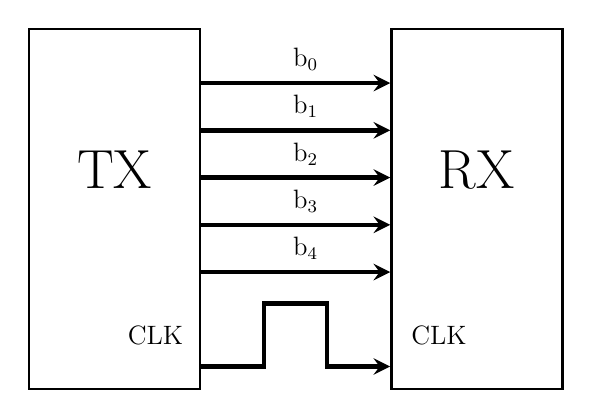
\begin{tikzpicture}[scale=0.8, transform shape]
            % Paths, nodes and wires:
            \node[shape=rectangle, draw, line width=1pt, minimum width=2.715cm, minimum height=5.715cm] at (1.375, 2.875){};
            \node[shape=rectangle, minimum width=0.465cm, minimum height=0.59cm] at (4.25, 2.25){} node[anchor=center, align=center, text width=0.077cm, inner sep=6pt] at (4.25, 2.25){\large $\mathrm{b_4}$};
            \draw[line width=1.6pt, -stealth] (2.75, 0.375) -- (3.75, 0.375) -| (3.75, 1.375) -- (4.75, 1.375) -| (4.75, 0.375) -- (5.75, 0.375);
            \draw[line width=1.6pt, -stealth] (2.75, 1.875) -- (5.75, 1.875);
            \draw[line width=1.6pt, -stealth] (2.75, 2.625) -- (5.75, 2.625);
            \draw[line width=1.6pt, -stealth] (2.75, 3.375) -- (5.75, 3.375);
            \node[shape=rectangle, minimum width=0.465cm, minimum height=0.59cm] at (4.25, 3){} node[anchor=center, align=center, text width=0.077cm, inner sep=6pt] at (4.25, 3){\large $\mathrm{b_3}$};
            \draw[line width=1.6pt, -stealth] (2.75, 4.125) -- (5.75, 4.125);
            \node[shape=rectangle, minimum width=0.465cm, minimum height=0.59cm] at (4.25, 3.75){} node[anchor=center, align=center, text width=0.077cm, inner sep=6pt] at (4.25, 3.75){\large $\mathrm{b_2}$};
            \draw[line width=1.6pt, -stealth] (2.75, 4.875) -- (5.75, 4.875);
            \node[shape=rectangle, minimum width=0.465cm, minimum height=0.59cm] at (4.25, 4.5){} node[anchor=center, align=center, text width=0.077cm, inner sep=6pt] at (4.25, 4.5){\large $\mathrm{b_1}$};
            \node[shape=rectangle, minimum width=0.465cm, minimum height=0.59cm] at (4.25, 5.25){} node[anchor=center, align=center, text width=0.077cm, inner sep=6pt] at (4.25, 5.25){\large $\mathrm{b_0}$};
            \node[shape=rectangle, minimum width=2.465cm, minimum height=1.965cm] at (1.375, 3.5){} node[anchor=center, align=center, text width=2.077cm, inner sep=6pt] at (1.375, 3.5){\Huge TX};
            \node[shape=rectangle, minimum width=1.215cm, minimum height=0.59cm] at (2, 0.875){} node[anchor=center, align=center, text width=0.827cm, inner sep=6pt] at (2, 0.875){\large CLK};
            \node[shape=rectangle, draw, line width=1pt, minimum width=2.715cm, minimum height=5.715cm] at (7.125, 2.875){};
            \node[shape=rectangle, minimum width=2.465cm, minimum height=1.965cm] at (7.125, 3.5){} node[anchor=center, align=center, text width=2.077cm, inner sep=6pt] at (7.125, 3.5){\Huge RX};
            \node[shape=rectangle, minimum width=1.215cm, minimum height=0.59cm] at (6.5, 0.875){} node[anchor=center, align=center, text width=0.827cm, inner sep=6pt] at (6.5, 0.875){\large CLK};
        \end{tikzpicture} 
        }
        \caption{Parallel Link Interface} \label{fig:parallel_link}
    \end{subfigure}
    \begin{subfigure}[b]{0.8\textwidth}
        \resizebox{\linewidth}{!}{
        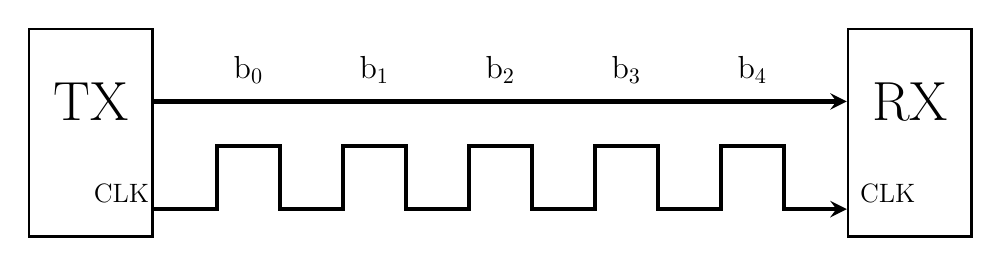
\begin{tikzpicture}[scale=0.8, transform shape]
            % Paths, nodes and wires:
            \draw[line width=1.6pt, -stealth] (2, 0.458) -- (3, 0.458) -- (3, 1.458) -- (4, 1.458) -- (4, 0.458) -- (5, 0.458) -- (5, 1.458) -- (6, 1.458) -- (6, 0.458) -- (7, 0.458) -- (7, 1.458) -- (8, 1.458) -- (8, 0.458) -- (9, 0.458) -- (9, 1.458) -- (10, 1.458) -- (10, 0.458) -- (11, 0.458) -- (11, 1.458) -- (12, 1.458) -- (12, 0.458) -- (13, 0.458);
            \node[shape=rectangle, minimum width=0.965cm, minimum height=0.965cm] at (3.5, 2.667){} node[anchor=center, align=center, text width=0.577cm, inner sep=6pt] at (3.5, 2.667){\Large $\mathrm{b_0}$};
            \node[shape=rectangle, minimum width=0.965cm, minimum height=0.965cm] at (5.5, 2.667){} node[anchor=center, align=center, text width=0.577cm, inner sep=6pt] at (5.5, 2.667){\Large $\mathrm{b_1}$};
            \node[shape=rectangle, minimum width=0.965cm, minimum height=0.965cm] at (7.5, 2.667){} node[anchor=center, align=center, text width=0.577cm, inner sep=6pt] at (7.5, 2.667){\Large $\mathrm{b_2}$};
            \node[shape=rectangle, minimum width=0.965cm, minimum height=0.965cm] at (9.5, 2.667){} node[anchor=center, align=center, text width=0.577cm, inner sep=6pt] at (9.5, 2.667){\Large $\mathrm{b_3}$};
            \node[shape=rectangle, minimum width=0.965cm, minimum height=0.965cm] at (11.5, 2.667){} node[anchor=center, align=center, text width=0.577cm, inner sep=6pt] at (11.5, 2.667){\Large $\mathrm{b_4}$};
            \node[shape=rectangle, draw, line width=1pt, minimum width=1.965cm, minimum height=3.298cm] at (1, 1.667){};
            \draw[line width=1.6pt, -stealth] (2, 2.167) -- (13, 2.167);
            \node[shape=rectangle, minimum width=1.798cm, minimum height=1.381cm] at (1, 2.167){} node[anchor=center, align=center, text width=1.41cm, inner sep=6pt] at (1, 2.167){\Huge TX};
            \node[shape=rectangle, minimum width=1.131cm, minimum height=0.715cm] at (1.417, 0.708){} node[anchor=center, align=center, text width=0.743cm, inner sep=6pt] at (1.417, 0.708){\large CLK};
            \node[shape=rectangle, draw, line width=1pt, minimum width=1.965cm, minimum height=3.298cm] at (14, 1.667){};
            \node[shape=rectangle, minimum width=1.798cm, minimum height=1.381cm] at (14, 2.167){} node[anchor=center, align=center, text width=1.41cm, inner sep=6pt] at (14, 2.167){\Huge RX};
            \node[shape=rectangle, minimum width=1.131cm, minimum height=0.715cm] at (13.583, 0.708){} node[anchor=center, align=center, text width=0.743cm, inner sep=6pt] at (13.583, 0.708){\large CLK};
        \end{tikzpicture}
        }
        \caption{ Serial Link Interface} \label{fig:serial_link}
    \end{subfigure}
    \caption{Communication link interfaces} \label{fig:comm_link_interfaces}
\end{figure}

High-speed serial links address these limitations by transmitting data sequentially, one bit at a time, over one or a small number of physical channels. By reducing the number of interconnects, serial architectures significantly simplify routing, eliminate inter-lane skew, and improve scalability with technology scaling.
However, with the decrease of the number of physical channels, the data rate per channel must increase to maintain the same aggregate throughput. This requires higher signaling frequencies, which results in tighter margins for signal intergrity~\cite{yang_serial_links_1998}, discussed in Section~\ref{sec:bg_signal_integrity}.

%Maybe refer that the downside is that you need to transmit at a higher frequency when using less wires

\subsection{Single-Ended and Differential Signaling}\label{sec:signaling}

In addition to the choice between parallel and serial transmission, the signaling scheme used on the physical channel plays a critical role in determining link robustness. In single-ended signaling, information is conveyed as a voltage referenced to a common ground.
The use of complementary conductors in differential transmission is illustrated in Figure~\ref{fig:differential_signaling}.
\begin{figure}[h]
    \centering
    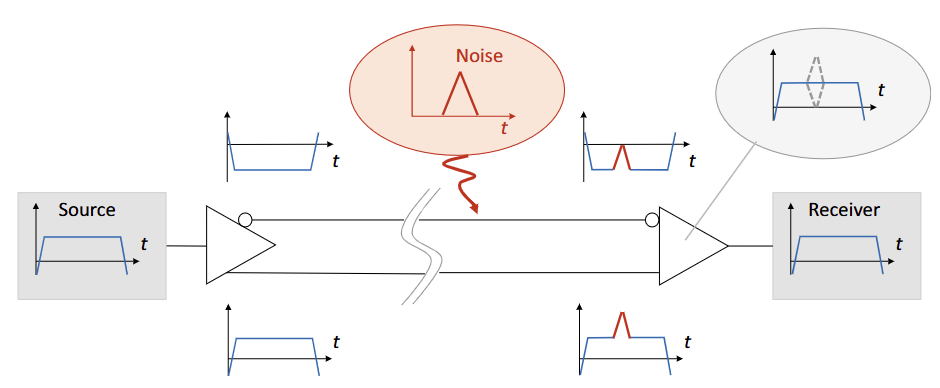
\includegraphics[width=0.8\textwidth]{chapter2/differential_signaling.png}
    \caption{Differential signaling. Reproduced from \cite{layout_fundamentals}}\label{fig:differential_signaling}
\end{figure}
While simple to implement, single-ended communication is highly sensitive to noise, supply fluctuations, and \ac{EMI}, particularly at high data rates. Differential signaling has therefore become the dominant communication scheme in high-speed serial links. In differential transmission, information is encoded in the voltage difference between two complementary signals~\cite{bogatin_SI,dally_poulton_1998}. The output signal is known as the differential-mode voltage, expressed in \eqref{eq:diff_mode_voltage}.

\begin{comment}
    
\begin{figure}
    \centering
    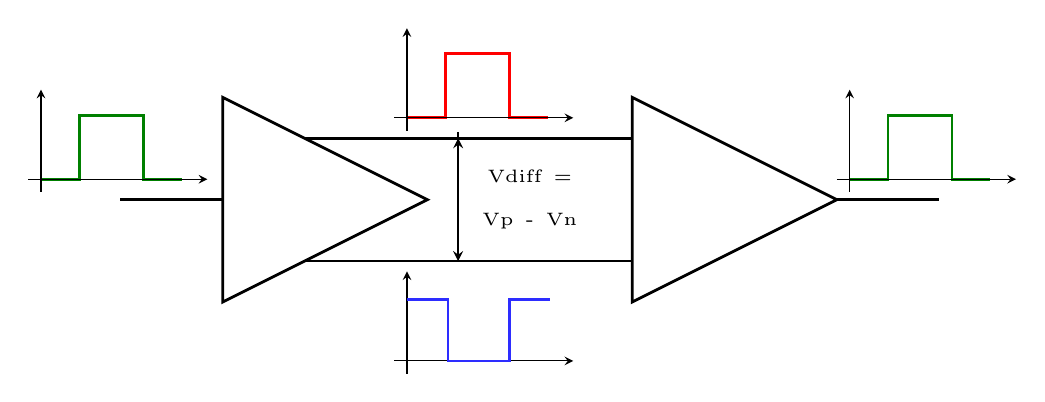
\begin{tikzpicture}[scale=1.3, transform shape]
        % Paths, nodes and wires:
        \draw[line width=1pt] (-2.525, 2.6) -- (-2.525, 0.6) -- (-0.525, 1.6) -- (-2.525, 2.6) -- cycle;
        \draw[line width=1pt] (-1.725, 2.2) -- (1.475, 2.2);
        \draw[line width=1pt] (-1.725, 1) -- (1.475, 1);
        \path[draw={rgb,255:red,255;green,0;blue,0}, line width=1pt] (-0.725, 2.4) -- (-0.35, 2.4) -- (-0.35, 3.025) -- (0.15, 3.025) -- (0.275, 3.025) -| (0.275, 2.4) -- (0.65, 2.4);
        \draw[stealth-] (-0.725, 3.275) -- (-0.725, 2.275);
        \draw[-stealth] (-0.85, 2.4) -- (0.9, 2.4);
        \draw[stealth-] (-0.725, 0.9) -- (-0.725, -0.1);
        \draw[-stealth] (-0.85, 0.025) -- (0.9, 0.025);
        \path[draw={rgb,255:red,45;green,45;blue,255}, line width=1pt] (-0.725, 0.625) -- (-0.325, 0.625) -| (-0.325, 0.025) -| (0.275, 0.125) -| (0.275, 0.625) -- (0.675, 0.625);
        \draw[line width=1pt] (-3.525, 1.6) -- (-2.525, 1.6);
        \path[draw={rgb,255:red,0;green,128;blue,0}, line width=1pt] (-4.3, 1.8) -- (-3.925, 1.8) -- (-3.925, 2.425) -- (-3.425, 2.425) -- (-3.3, 2.425) -| (-3.3, 1.8) -- (-2.925, 1.8);
        \draw[stealth-] (-4.3, 2.675) -- (-4.3, 1.675);
        \draw[-stealth] (-4.425, 1.8) -- (-2.675, 1.8);
        \path[draw={rgb,255:red,0;green,128;blue,0}, line width=1pt] (3.6, 1.8) -- (3.975, 1.8) -- (3.975, 2.425) -- (4.475, 2.425) -- (4.6, 2.425) -| (4.6, 1.8) -- (4.975, 1.8);
        \draw[stealth-] (3.6, 2.675) -- (3.6, 1.675);
        \draw[-stealth] (3.475, 1.8) -- (5.225, 1.8);
        \draw[line width=1pt] (1.475, 2.6) -- (1.475, 0.6) -- (3.475, 1.6) -- (1.475, 2.6) -- cycle;
        \draw[line width=1pt] (3.475, 1.6) -- (4.475, 1.6);
        \draw[line width=0.6pt, stealth-stealth] (-0.225, 2.2) -| (-0.225, 1);
        \node[shape=rectangle, minimum width=1.865cm, minimum height=0.565cm] at (0.475, 1.6){} node[anchor=center, align=center, text width=1.477cm, inner sep=6pt] at (0.475, 1.6){\tiny Vdiff = Vp - Vn};
    \end{tikzpicture}
    \caption{Differential signaling}\label{fig:differential_signaling}
\end{figure}

\end{comment}



\begin{equation}
    V_{DM} = V_{D+} - V_{D-}
    \label{eq:diff_mode_voltage}
\end{equation}

This approach suppresses common-mode noise, reduces sensitivity to ground potential variations, and significantly lowers electromagnetic emissions \cite{bogatin_SI,dally_poulton_1998}. Furthermore, differential signaling allows smaller voltage swings while preserving noise margins, enabling faster edge rates and reduced dynamic power consumption, which balances out the downside of having two physical channels and added circuit complexity.

\subsection{Non Return to Zero Encoding} \label{sec:nrz_encoding}

\begin{comment}
    - NRZ is a digital line coding technique in which the signal remain constant throughout each bit period without returning to a zero reference level
    - NRZ is simple to implement and bandwidth efficient
    - NRZ encodes one bit per symbol, its minimum required channel bandwidth is the Nyquist frequency, which is half of the bit rate
    - NRZ is the same as Pulse Amplitude Modulation 2-level (PAM2), since it uses two distinct voltage levels to represent binary data
    - NRZ/PAM2 has two symbol levels, two rising/falling edges, two distinct transistions, 1 eye diagram per UI, 50\% average transition density
    - Transitions between levels in a NRZ/PAM2 signal are smooth
    - NRZ/PAM2 has better error correction performance, more resistance to noise, lower SNR and BER qhen compared to multi-level modulation schemes such as PAM4
    - NRZ/PAM2 has a simple structure, does not rqeuite clock recovery circuit
    - NRZ/PAM2 has a limited bandwidth, which can be a disadvantage in high-speed communication systems, especially when compared to multi-level modulation schemes such as PAM4, which can transmit more bits per symbol and achieve higher data rates within the same bandwidth
\end{comment}

\ac{NRZ} is a digital line coding technique in which the transmitted signal is held constant at one of two voltage levels throughout the entirety of each bit period, without returning to a zero reference level between consecutive bits~\cite{razavi_NRZ_PAM4,zamir2018_nrz_pam4}.
An example of this two-level waveform is shown in Figure~\ref{fig:nrz_waveform}, illustrating the high and low logic levels and the transitions between them.

\begin{figure}[H]
    \centering
    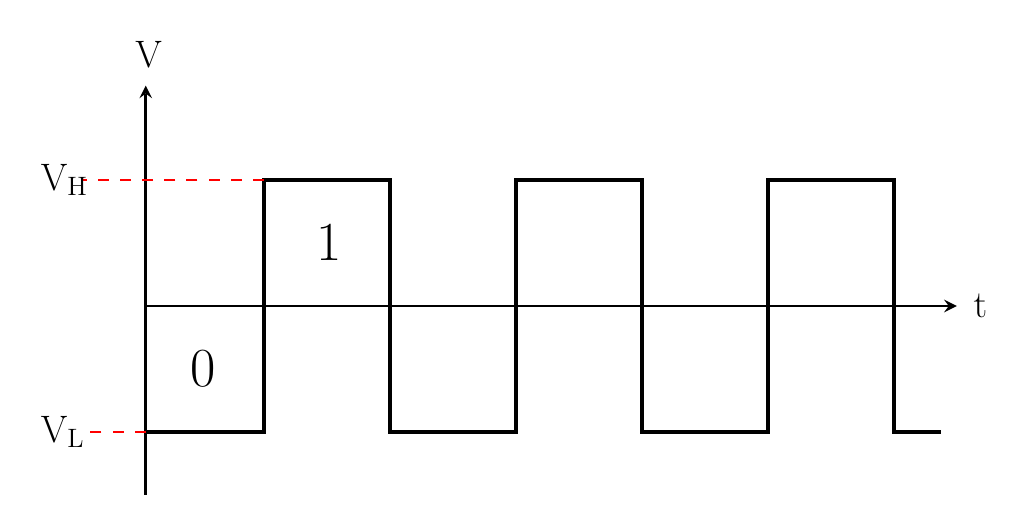
\begin{tikzpicture}[scale=0.8, transform shape]
        % Paths, nodes and wires:
        \draw[line width=1pt, -stealth] (1.875, 3) -- (14.75, 3);
        \node[shape=rectangle, minimum width=0.715cm, minimum height=0.715cm] at (15.125, 3){} node[anchor=center, align=center, text width=0.327cm, inner sep=6pt] at (15.125, 3){\LARGE t};
        \draw[line width=1.5pt] (1.875, 1) -- (3.625, 1) -| (3.75, 5) -- (5.75, 5) -- (5.75, 1) |- (7.75, 1) -| (7.75, 5) -- (9.75, 5) -- (9.75, 1) |- (11.75, 1) -| (11.75, 5) -- (13.75, 5) -| (13.75, 1) -- (14.5, 1);
        \node[shape=rectangle, minimum width=0.715cm, minimum height=0.715cm] at (2.75, 2){} node[anchor=center, align=center, text width=0.327cm, inner sep=6pt] at (2.75, 2){\Huge 0};
        \node[shape=rectangle, minimum width=0.715cm, minimum height=0.715cm] at (4.75, 4){} node[anchor=center, align=center, text width=0.327cm, inner sep=6pt] at (4.75, 4){\Huge 1};
        \draw[line width=1pt, -stealth] (1.875, -0) -| (1.875, 6.5);
        \node[shape=rectangle, minimum width=0.715cm, minimum height=0.715cm] at (1.875, 7){} node[anchor=center, align=center, text width=0.327cm, inner sep=6pt] at (1.875, 7){\LARGE V};
        \path[draw={rgb,255:red,255;green,0;blue,0}, line width=1pt, dash pattern={on 4pt off 4pt}] (3.75, 5) -- (0.875, 5);
        \path[draw={rgb,255:red,255;green,0;blue,0}, line width=1pt, dash pattern={on 4pt off 4pt}] (1.875, 1) -- (0.875, 1);
        \node[shape=rectangle, minimum width=0.715cm, minimum height=0.715cm] at (0.375, 5){} node[anchor=center, align=center, text width=0.327cm, inner sep=6pt] at (0.375, 5){\LARGE $\mathrm{V_H}$};
        \node[shape=rectangle, minimum width=0.715cm, minimum height=0.715cm] at (0.375, 1){} node[anchor=center, align=center, text width=0.327cm, inner sep=6pt] at (0.375, 1){\LARGE $\mathrm{V_L}$};
    \end{tikzpicture}
    \caption{NRZ waveform}\label{fig:nrz_waveform}
\end{figure}

Since \ac{NRZ} encodes exactly one bit per transmitted symbol, its minimum required channel bandwidth is given by the Nyquist frequency, corresponding to half of the bit rate~\cite{razavi_NRZ_PAM4}:

\begin{equation}
    f_{Nyquist} = \frac{R_b}{2},
    \label{eq:nyquist_freq}
\end{equation}

\noindent where $R_b$ is the bit rate. For a 10\,Gb/s \ac{NRZ} link such as USB 3.2 Gen 2, this corresponds to a Nyquist frequency of 5\,GHz.
The frequency-domain characteristics of an \ac{NRZ} signal are illustrated by its power spectral density in Figure~\ref{fig:nrz_psd}.

\begin{figure}[H]
    \centering
    \begin{tikzpicture}[scale=0.6]
        % Coordinates
        \coordinate (A) at (0.00, 0.00);
        \coordinate (B) at (1.48, 0.99);
        \coordinate (C) at (1.00, 0.00);
        \coordinate (D) at (0.75, 1.00);
        \coordinate (E) at (3.00, 0.00);
        \coordinate (F) at (2.25, 1.00);
        \coordinate (G) at (2.00, 0.00);
        \coordinate (H) at (4.50, 2.00);
        \coordinate (I) at (4.25, 0.00);
        \coordinate (J) at (3.50, 2.00);
        \coordinate (K) at (6.00, 0.00);
        \coordinate (L) at (5.50, 2.00);
        \coordinate (M) at (4.75, 0.00);
        \coordinate (N) at (7.50, 3.00);
        \coordinate (O) at (7.25, 0.00);
        \coordinate (P) at (6.50, 3.00);
        \coordinate (Q) at (9.00, -0.01);
        \coordinate (R) at (8.50, 3.00);
        \coordinate (S) at (7.75, 0.00);
        \coordinate (T) at (11.52, 6.00);
        \coordinate (U) at (10.50, 0.00);
        \coordinate (V) at (9.25, 6.00);
        \coordinate (W) at (14.00, 0.01);
        \coordinate (X) at (13.75, 6.00);
        \coordinate (Y) at (12.47, 0.05);
        \coordinate (AA) at (15.50, 3.00);
        \coordinate (AB) at (15.25, 0.00);
        \coordinate (AC) at (14.50, 3.00);
        \coordinate (AD) at (16.50, 3.00);
        \coordinate (AE) at (15.75, 0.00);
        \coordinate (AF) at (14.00, 0.00);
        \coordinate (AG) at (17.00, -0.01);
        \coordinate (AI) at (17.00, -0.01);
        \coordinate (AJ) at (18.25, -0.01);
        \coordinate (AK) at (17.50, 1.99);
        \coordinate (AL) at (18.50, 1.99);
        \coordinate (AM) at (19.50, 1.99);
        \coordinate (AN) at (18.75, -0.01);
        \coordinate (AO) at (20.00, -0.01);
        \coordinate (AP) at (20.00, -0.01);
        \coordinate (AQ) at (21.48, 0.98);
        \coordinate (AR) at (21.00, -0.01);
        \coordinate (AS) at (20.75, 0.99);
        \coordinate (AT) at (22.25, 0.99);
        \coordinate (AU) at (22.00, -0.01);
        \coordinate (AV) at (23.00, -0.01);
        \coordinate (AW) at (23.75, 0.00);
        \coordinate (AX) at (11.50, -0.01);
        \coordinate (AY) at (11.50, 7.25);

        % Drawing
        \draw (A) .. controls (1.00, 0.00) and (0.75, 1.00) .. (B);
        \draw (B) .. controls (2.25, 1.00) and (2.00, 0.00) .. (E);
        \draw (E) .. controls (4.25, 0.00) and (3.50, 2.00) .. (H);
        \draw (H) .. controls (5.50, 2.00) and (4.75, 0.00) .. (K);
        \draw (K) .. controls (7.25, 0.00) and (6.50, 3.00) .. (N);
        \draw (N) .. controls (8.50, 3.00) and (7.75, 0.00) .. (Q);
        \draw (Q) .. controls (10.50, 0.00) and (9.25, 6.00) .. (T);
        \draw (T) .. controls (13.75, 6.00) and (12.47, 0.05) .. (W);
        \draw (AF) .. controls (15.25, 0.00) and (14.50, 3.00) .. (AA);
        \draw (AA) .. controls (16.50, 3.00) and (15.75, 0.00) .. (AG);
        \draw (AI) .. controls (18.25, -0.01) and (17.50, 1.99) .. (AL);
        \draw (AL) .. controls (19.50, 1.99) and (18.75, -0.01) .. (AO);
        \draw (AP) .. controls (21.00, -0.01) and (20.75, 0.99) .. (AQ);
        \draw (AQ) .. controls (22.25, 0.99) and (22.00, -0.01) .. (AV);
        \draw[->, >={Stealth[scale=2]}, thick] (A) -- node[right, font=\large, text=black, at end] {f}  node[above, midway] {} (AW);
        \draw[->, >={Stealth[scale=2]}, thick] (AX) -- node[above, font=\large, text=black, at end] {$S_x(f)$}  node[below, text=black, at start] {0} (AY);
        \draw[thick, dashed] (T) -- (V);
        \node[left, font=\large, text=black] at (V) {$T_b$};
        \node[below, font=\large, text=black] at (AF) {$\frac{1}{T_b}$};
        \node[below, font=\large, text=black] at (AI) {$\frac{2}{T_b}$};
        \node[below, font=\large, text=black] at (AP) {$\frac{3}{T_b}$};
    \end{tikzpicture}
    \caption{Power spectral density of a \ac{NRZ} signal}\label{fig:nrz_psd}
\end{figure}

In terms of modulation, \ac{NRZ} is equivalent to \ac{PAM2}, since both encode binary data using two distinct voltage levels. As a \ac{PAM2} scheme, \ac{NRZ} signaling is characterized by two symbol levels, two possible transitions (rising and falling), a single eye diagram per \ac{UI}, and a maximum average transition density of 50\%, corresponding to the case of alternating bit patterns~\cite{razavi_NRZ_PAM4}. Transitions between the two voltage levels in a \ac{NRZ}/\ac{PAM2} signal are smooth, rather than instantaneous, due to the finite bandwidth of the \ac{TX}, channel, and receiver.
Figure~\ref{fig:nrz_and_pam4} compares the voltage levels used in \ac{NRZ} and \ac{PAM4} signaling.

\begin{figure}[H]
    \centering
    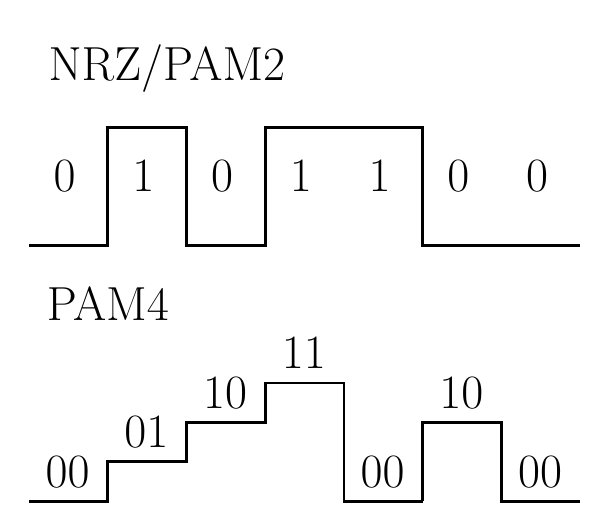
\begin{tikzpicture}[transform shape]
        % Paths, nodes and wires:
        \draw[line width=1pt] (5, -0) -| (4, 1.5) -- (3, 1.5) -| (3, 1) -- (2, 1) -| (2, 0.5) -- (1, 0.5) -| (1, -0) -- (-0, -0);
        \draw[line width=1pt] (-0, 3.25) -- (1, 3.25) -| (1, 4.75) -- (2, 4.75) -| (2, 3.25) -- (3, 3.25) -- (3, 4.75) -- (5, 4.75) -- (5, 3.25) -- (7, 3.25);
        \draw[line width=1pt] (5, -0) -| (5, 1) -- (6, 1) -| (6, 0.5) -| (6, -0) -- (7, -0);
        \node[shape=rectangle, minimum width=0.465cm, minimum height=0.715cm] at (0.25, 4.125){} node[anchor=center, align=center, text width=0.077cm, inner sep=6pt] at (0.25+0.1, 4.125){\LARGE 0};
        \node[shape=rectangle, minimum width=0.465cm, minimum height=0.715cm] at (1.25, 4.125){} node[anchor=center, align=center, text width=0.077cm, inner sep=6pt] at (1.25+0.1, 4.125){\LARGE 1};
        \node[shape=rectangle, minimum width=0.465cm, minimum height=0.715cm] at (2.25, 4.125){} node[anchor=center, align=center, text width=0.077cm, inner sep=6pt] at (2.25+0.1, 4.125){\LARGE 0};
        \node[shape=rectangle, minimum width=0.465cm, minimum height=0.715cm] at (6.25, 4.125){} node[anchor=center, align=center, text width=0.077cm, inner sep=6pt] at (6.25+0.1, 4.125){\LARGE 0};
        \node[shape=rectangle, minimum width=0.465cm, minimum height=0.715cm] at (3.25, 4.125){} node[anchor=center, align=center, text width=0.077cm, inner sep=6pt] at (3.25+0.1, 4.125){\LARGE 1};
        \node[shape=rectangle, minimum width=0.465cm, minimum height=0.715cm] at (4.25, 4.125){} node[anchor=center, align=center, text width=0.077cm, inner sep=6pt] at (4.25+0.1, 4.125){\LARGE 1};
        \node[shape=rectangle, minimum width=0.465cm, minimum height=0.715cm] at (5.25, 4.125){} node[anchor=center, align=center, text width=0.077cm, inner sep=6pt] at (5.25+0.1, 4.125){\LARGE 0};
        \node[shape=rectangle, minimum width=0.465cm, minimum height=0.715cm] at (0.25, 0.375){} node[anchor=center, align=center, text width=0.077cm, inner sep=6pt] at (0.25, 0.375){\LARGE 00};
        \node[shape=rectangle, minimum width=0.465cm, minimum height=0.715cm] at (1.25, 0.875){} node[anchor=center, align=center, text width=0.077cm, inner sep=6pt] at (1.25, 0.875){\LARGE 01};
        \node[shape=rectangle, minimum width=0.465cm, minimum height=0.715cm] at (2.25, 1.375){} node[anchor=center, align=center, text width=0.077cm, inner sep=6pt] at (2.25, 1.375){\LARGE 10};
        \node[shape=rectangle, minimum width=0.465cm, minimum height=0.715cm] at (3.25, 1.875){} node[anchor=center, align=center, text width=0.077cm, inner sep=6pt] at (3.25, 1.875){\LARGE 11};
        \node[shape=rectangle, minimum width=0.465cm, minimum height=0.715cm] at (4.25, 0.375){} node[anchor=center, align=center, text width=0.077cm, inner sep=6pt] at (4.25, 0.375){\LARGE 00};
        \node[shape=rectangle, minimum width=0.465cm, minimum height=0.715cm] at (6.25, 0.375){} node[anchor=center, align=center, text width=0.077cm, inner sep=6pt] at (6.25, 0.375){\LARGE 00};
        \node[shape=rectangle, minimum width=0.465cm, minimum height=0.715cm] at (5.25, 1.375){} node[anchor=center, align=center, text width=0.077cm, inner sep=6pt] at (5.25, 1.375){\LARGE 10};
        \node[shape=rectangle, minimum width=1.965cm, minimum height=0.715cm] at (1, 2.5){} node[anchor=center, align=center, text width=1.577cm, inner sep=6pt] at (1, 2.5){\LARGE PAM4};
        \node[shape=rectangle, minimum width=3.465cm, minimum height=0.715cm] at (1.75, 5.5){} node[anchor=center, align=center, text width=3.077cm, inner sep=6pt] at (1.75, 5.5){\LARGE NRZ/PAM2};
    \end{tikzpicture}
    \caption{NRZ and PAM4}\label{fig:nrz_and_pam4}
\end{figure}

Compared to multi-level modulation schemes such as \ac{PAM4}, \ac{NRZ}/\ac{PAM2} offers superior error correction performance, greater resistance to noise, and requires a lower \ac{SNR} to achieve a given \ac{BER}~\cite{razavi_NRZ_PAM4,zamir2018_nrz_pam4}, owing to its simpler encoding, with only two symbol levels.

%Compared to multi-level modulation schemes such as \ac{PAM4}, \ac{NRZ}/\ac{PAM2} offers superior error correction performance, greater resistance to noise, and requires a lower \ac{SNR} to achieve a given \ac{BER}~\cite{razavi_NRZ_PAM4,zamir2018_nrz_pam4}, owing to the larger voltage margin between its two symbol levels.

The main disadvantage of \ac{NRZ}/\ac{PAM2} lies in its limited spectral efficiency: since only one bit is conveyed per symbol, achieving higher data rates requires proportionally higher channel bandwidth. This is a significant limitation in high-speed communication systems, especially when compared to multi-level modulation schemes such as \ac{PAM4}, which encode multiple bits per symbol and can therefore achieve higher data rates within the same channel bandwidth~\cite{razavi_NRZ_PAM4,chen_cml_review_2026}, at the cost of reduced noise margin and increased receiver complexity.  

%I would add some figure to explain the NRZ vs PAM 4. Maybe an eye diagram or signal constelation

%\subsection{High Speed Serial Links}
%The continuous growth in data throughput requirements of modern electronic systems has made high-speed communication links a fundamental enabler of contemporary digital platforms. Applications such as high-performance computing, mass storage, consumer peripherals, and data center interconnects require sustained data rates in the multi-gigabit-per-second range while maintaining strict constraints on power consumption, electromagnetic interference, and physical interconnect complexity \cite{razavi, baker}.
%As semiconductor technology has scaled, the switching speed of transistors has increased significantly However, the performance of interconnects has not scaled at the same pace. Consequently, communication between integrated circuits and system components has become a dominant bottleneck. In many modern systems, overall performance is limited not by logic speed but by the ability to reliably transmit data across electrical interconnects, motivating the development of high-speed link architectures optimized for signal integrity and energy efficiency.

\subsection{\acs{USB} Standard}\label{subsec:usb_standard}
    
The \ac{USB} is an industry standard for digital data transmission between electronic devices, first introduced in 1996. It is developed and maintained by the \ac{USB-IF}, a consortium of companies that promotes, supports, and certifies compliance with the \ac{USB} standard across the industry. The standard specifies the architecture of the communication link established between connected devices, encompassing both the physical interfaces used and the communication protocols that govern data exchange over them.

Since its introduction, \ac{USB} has undergone several major revisions, progressively increasing its supported data rates: from \ac{USB} 1.0, released in 1996 and supporting data rates of up to 12\,Mb/s, to the most recent \ac{USB} 4 standard, released in 2019, which supports data transfer rates of up to 40\,Gb/s. Across all of these revisions, \ac{USB} has consistently relied on differential signaling to transmit data over a pair of conductors, as discussed in Section~\ref{sec:signaling}, owing to its inherent noise immunity and suitability for high-speed operation.

\begin{figure}[H]
    \centering
    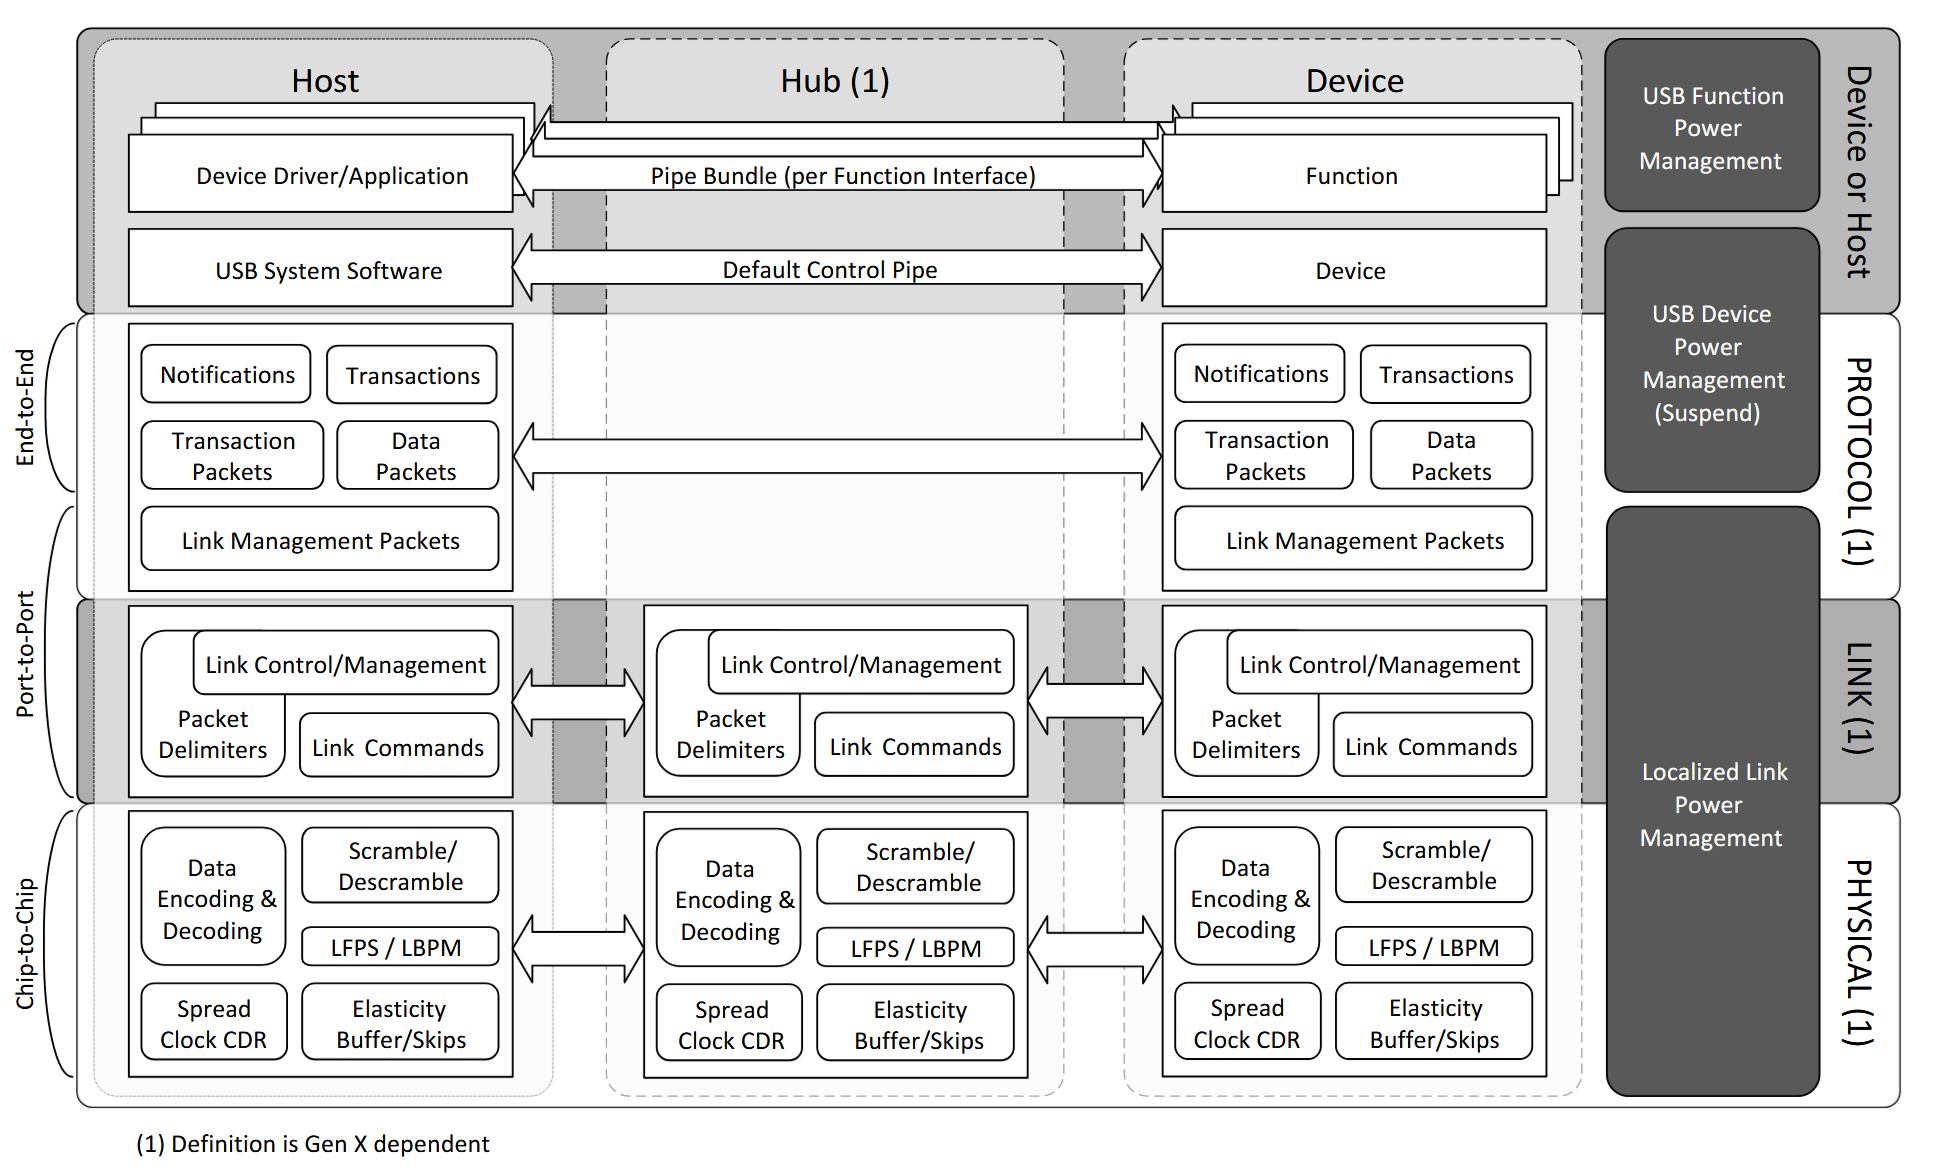
\includegraphics[width=1\textwidth]{figures/chapter2/usb32_layers.png}
    \caption{USB 3.2 layers. Reproduced from \cite{usb32_specs}}\label{fig:usb32_layers}
\end{figure}

Architecturally, \ac{USB} operates through three primary, interdependent layers: the \ac{PHY}, the link layer, and the protocol layer, as illustrated in Figure~\ref{fig:usb32_layers}. The \ac{PHY} is responsible for the electrical transmission and reception of data over the physical medium, the link layer manages framing, flow control, and link-level management functions, and the protocol layer handles end-to-end communication between the host and device applications.

\subsubsection{\acs{USB} 3.2 \acs{PHY} Layer}\label{sec:usb32_phy_layer}

The work presented in this dissertation targets compliance with the \ac{USB} 3.2 Gen 2 standard, commercially marketed as SuperSpeed \ac{USB}, introduced with \ac{USB} 3.1 in 2013 and subsequently incorporated into the \ac{USB} 3.2 specification.. The \ac{USB} 3.2 Gen 2 standard specifies a maximum data rate of 10\,Gb/s, achieved through the use of \ac{NRZ} signaling, discussed in Section~\ref{sec:nrz_encoding}, transmitted over a differential pair of conductors.

The \ac{USB} 3.2 SuperSpeed \ac{PHY} defines the underlying signaling technology used to implement this data rate, and is responsible for the encoding and decoding of data, as well as its transmission and reception over the physical channel. In addition to defining the signaling technology itself, the \ac{PHY} layer specifies the electrical requirements that a compliant \ac{TX} and receiver must satisfy, discussed in Section~\ref{sec:usb32_specs}.

\section{Signal Integrity}\label{sec:bg_signal_integrity}

When a signal is transmitted through an electrical channel, it inevitably undergoes various forms of degradation, arising from the physical properties of the interconnect itself as well as from the surrounding electrical environment. This degradation can manifest as attenuation, distortion, noise, and crosstalk, all of which contribute to compromising the integrity of the transmitted signal by the time it reaches the receiver~\cite{bogatin_SI,zamir2018_nrz_pam4}. This section discusses the main mechanisms of signal degradation relevant to high-speed serial links, and how to characterize their impact on the transmitted signal.

\subsection{Inter-Symbol Interference}\label{sec:isi_detailed}

\ac{ISI} is a form of signal distortion in which the energy associated with one transmitted symbol interferes with subsequent symbols, causing the signal to spread beyond its allotted time interval. Specifically, the energy transmitted during a given \ac{UI}, the time interval defined for sampling an individual bit, spreads into neighboring \acp{UI}, so that the waveform observed at the receiver during any given bit period is no longer determined solely by the symbol transmitted in that interval, but also carries residual contributions from adjacent symbols.

This superposition of energy from neighboring symbols can result in an incorrect interpretation of the transmitted data at the receiver: the bit sampled at the decision point may be misread due to the overlap of adjacent symbols with the intended sample, leading to an increased \ac{BER}. Fundamentally, \ac{ISI} arises from the bandwidth-limited and frequency-dependent response of the channel, whereby different spectral components of the transmitted signal experience different attenuation and phase delay, causing each symbol to spread into neighboring \acsp{UI}~\cite{zamir2018_nrz_pam4}.

\subsection{Transmission Lines and Channel Characterization}\label{sec:transmission_lines}

At multi-gigabit data rates, the physical interconnect between the \ac{TX} and receiver can no longer be treated as an ideal connection, but must instead be considered as a transmission line whose electrical properties influence the propagated signal. In practice, the channel exhibits a frequency-dependent response that tends to attenuate the higher-frequency components of the transmitted waveform more strongly than its lower-frequency content, effectively introducing a low-pass behavior, as illustrated in Figure~\ref{fig:nrz_psd_filtered}. 

\begin{figure}[H]
    \centering
    \begin{tikzpicture}[scale=0.6]
        % Coordinates
        \coordinate (A) at (0.00, 0.00);
        \coordinate (B) at (1.48, 0.99);
        \coordinate (C) at (1.00, 0.00);
        \coordinate (D) at (0.75, 1.00);
        \coordinate (E) at (3.00, 0.00);
        \coordinate (F) at (2.25, 1.00);
        \coordinate (G) at (2.00, 0.00);
        \coordinate (H) at (4.50, 2.00);
        \coordinate (I) at (4.25, 0.00);
        \coordinate (J) at (3.50, 2.00);
        \coordinate (K) at (6.00, 0.00);
        \coordinate (L) at (5.50, 2.00);
        \coordinate (M) at (4.75, 0.00);
        \coordinate (N) at (7.50, 3.00);
        \coordinate (O) at (7.25, 0.00);
        \coordinate (P) at (6.50, 3.00);
        \coordinate (Q) at (9.00, -0.01);
        \coordinate (R) at (8.50, 3.00);
        \coordinate (S) at (7.75, 0.00);
        \coordinate (T) at (11.52, 6.00);
        \coordinate (U) at (10.50, 0.00);
        \coordinate (V) at (9.25, 6.00);
        \coordinate (W) at (14.00, 0.01);
        \coordinate (X) at (13.75, 6.00);
        \coordinate (Y) at (12.47, 0.05);
        \coordinate (AA) at (15.50, 3.00);
        \coordinate (AB) at (15.25, 0.00);
        \coordinate (AC) at (14.50, 3.00);
        \coordinate (AD) at (16.50, 3.00);
        \coordinate (AE) at (15.75, 0.00);
        \coordinate (AF) at (14.00, 0.00);
        \coordinate (AG) at (17.00, -0.01);
        \coordinate (AI) at (17.00, -0.01);
        \coordinate (AJ) at (18.25, -0.01);
        \coordinate (AK) at (17.50, 1.99);
        \coordinate (AL) at (18.50, 1.99);
        \coordinate (AM) at (19.50, 1.99);
        \coordinate (AN) at (18.75, -0.01);
        \coordinate (AO) at (20.00, -0.01);
        \coordinate (AP) at (20.00, -0.01);
        \coordinate (AQ) at (21.48, 0.98);
        \coordinate (AR) at (21.00, -0.01);
        \coordinate (AS) at (20.75, 0.99);
        \coordinate (AT) at (22.25, 0.99);
        \coordinate (AU) at (22.00, -0.01);
        \coordinate (AV) at (23.00, -0.01);
        \coordinate (AW) at (23.75, 0.00);
        \coordinate (AX) at (11.50, -0.01);
        \coordinate (AY) at (11.50, 7.25);

        % Drawing
        \draw[dashed, fill=lightgray] (10,0) rectangle (13,6.75);
        \draw (A) .. controls (1.00, 0.00) and (0.75, 1.00) .. (B);
        \draw (B) .. controls (2.25, 1.00) and (2.00, 0.00) .. (E);
        \draw (E) .. controls (4.25, 0.00) and (3.50, 2.00) .. (H);
        \draw (H) .. controls (5.50, 2.00) and (4.75, 0.00) .. (K);
        \draw (K) .. controls (7.25, 0.00) and (6.50, 3.00) .. (N);
        \draw (N) .. controls (8.50, 3.00) and (7.75, 0.00) .. (Q);
        \draw (Q) .. controls (10.50, 0.00) and (9.25, 6.00) .. (T);
        \draw (T) .. controls (13.75, 6.00) and (12.47, 0.05) .. (W);
        \draw (AF) .. controls (15.25, 0.00) and (14.50, 3.00) .. (AA);
        \draw (AA) .. controls (16.50, 3.00) and (15.75, 0.00) .. (AG);
        \draw (AI) .. controls (18.25, -0.01) and (17.50, 1.99) .. (AL);
        \draw (AL) .. controls (19.50, 1.99) and (18.75, -0.01) .. (AO);
        \draw (AP) .. controls (21.00, -0.01) and (20.75, 0.99) .. (AQ);
        \draw (AQ) .. controls (22.25, 0.99) and (22.00, -0.01) .. (AV);
        \draw[->, >={Stealth[scale=2]}, thick] (A) -- node[right, font=\large, text=black, at end] {f}  node[above, midway] {} (AW);
        \draw[->, >={Stealth[scale=2]}, thick] (AX) -- node[above, text=black, at end] {$S_x(f)$}  node[below, text=black, at start] {0} (AY);
        \draw[thick, dashed] (T) -- (V);
        \node[left, black] at (V) {$T_b$};
        \node[below, black] at (AF) {$\frac{1}{T_b}$};
        \node[below, black] at (AI) {$\frac{2}{T_b}$};
        \node[below, black] at (AP) {$\frac{3}{T_b}$};
    \end{tikzpicture}
    \caption{Power spectral density of a \ac{NRZ} signal with a low-pass filter applied}\label{fig:nrz_psd_filtered}
\end{figure}

Since these high-frequency components are responsible for preserving sharp transitions in an \ac{NRZ} signal, their attenuation leads to slower edges, waveform distortion, and ultimately increased \ac{ISI}. Consequently, characterizing the transmission channel in the frequency domain is essential for evaluating its effect on signal integrity and determining the impact it has at the \ac{TX}. The following subsections therefore introduce the principal channel-characterization losses and metrics.

\subsubsection{Insertion Loss}\label{sec:insertion_loss}

Insertion loss refers to the reduction in signal power that occurs as a signal propagates through a channel, and quantifies how much weaker a signal becomes after a given transmission line, or other channel element, is inserted into the signal path. This power reduction arises from several distinct physical loss mechanisms associated with the channel, such as dielectric losses, conductor losses, and reflection losses~\cite{bogatin_SI}.

% mostrar equação e falar que é medido em dB

Dielectric losses occur when a portion of the signal's energy is absorbed by the dielectric material surrounding the channel's conductors; this loss mechanism becomes progressively more significant as frequency increases, since the dielectric absorption coefficient itself grows with frequency. Conductor losses occur when a portion of the signal's energy is dissipated as heat within the channel conductors themselves, as a direct consequence of their finite electrical resistance, which similarly increases at high frequency due to the skin effect\cite{zamir2018_nrz_pam4}. 

% add figura sobre reflection loss

Reflection losses occur when a portion of the signal's energy is reflected back toward the \ac{TX} due to impedance mismatches or discontinuities along the channel, rather than being delivered to the receiver~\cite{bogatin_SI}.

Taken together, these loss mechanisms all increase with frequency, which is particularly problematic for high-speed serial links: since the high-frequency spectral content of the transmitted signal is primarily responsible for producing sharp, well-defined signal transitions~\cite{razavi_NRZ_PAM4,zamir2018_nrz_pam4}, the frequency-dependent nature of insertion loss disproportionately attenuates precisely the components of the signal needed to preserve fast, clean edges, directly motivating the need for a compensation mechanism such as \ac{TX} equalization, discussed in Section~\ref{sec:equalization}.

\subsubsection{Return Loss}\label{sec:return_loss}

Return loss is a measure of the fraction of the transmitted signal that is reflected back toward the \ac{TX} due to impedance mismatches or discontinuities along the channel~\cite{bogatin_SI}. These reflected signals travel back along the channel and can subsequently interfere with the forward-propagating transmitted signal, introducing additional distortion beyond that caused by insertion loss alone.

\subsubsection{Impedance Matching}\label{sec:impedance_matching_detailed}

To minimize the losses caused by signal reflections, the impedance discontinuities that give rise to them should be minimized wherever possible. In practice, this is achieved through impedance matching, that is, by designing the output impedance of the transmitting circuit to be as close as possible to the characteristic impedance of the channel. When these two impedances are equal, the channel presents no discontinuity to the signal at the \ac{TX} interface, and the fraction of signal power reflected back toward the \ac{TX} is minimized~\cite{bogatin_SI,chen_switchable_cml_2016}.

\subsubsection{Jitter}\label{sec:jitter_detailed}

Jitter refers to the deviation of signal transitions from their ideal, intended positions in time. It can be caused by a variety of mechanisms, including impedance mismatches, crosstalk between neighboring signal paths, and frequency-dependent losses such as the dielectric losses described in Section~\ref{sec:insertion_loss}. Regardless of its origin, jitter ultimately results in errors during the bit sampling process at the receiver, since transitions that occur earlier or later than expected reduce the effective timing margin available for correct sampling, thereby increasing the \ac{BER}~\cite{yang_serial_links_1998}.
The deviation of actual signal transitions from their ideal timing positions is illustrated in Figure~\ref{fig:jitter_example}.

\begin{figure}[H]
    \centering
    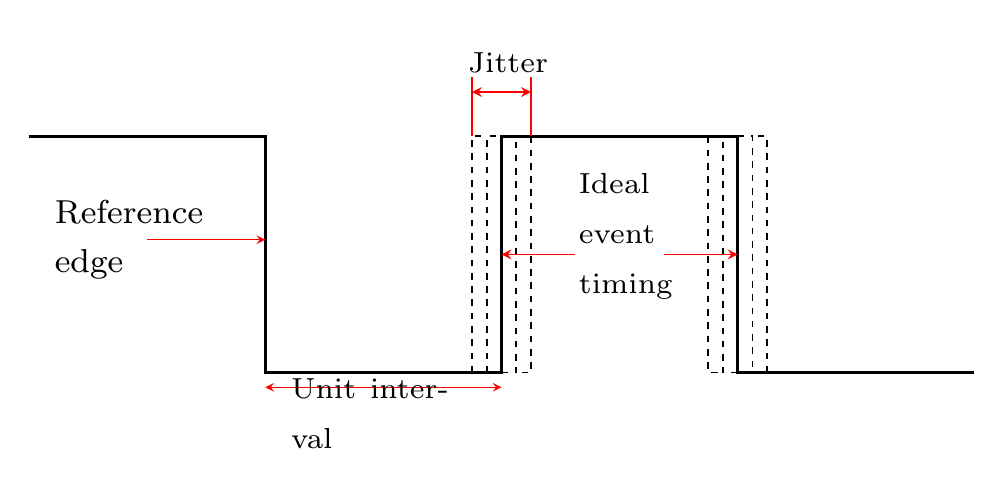
\begin{tikzpicture}[scale=1.5, transform shape]
        % Paths, nodes and wires:
        \draw[line width=1pt] (-4, 2) -- (-4, 2) -- (-2.5, 2) -- (-2, 2) -- (-2, -0) -- (0, -0) -- (0, 2) -- (2, 2) -- (2, -0) -- (4, -0);
        \draw[line width=0.6pt, dash pattern={on 2.4pt off 2.4pt}] (-0.25, -0) -| (-0.25, 2) -- (-0.125, 2);
        \draw[line width=0.6pt, dash pattern={on 2.4pt off 2.4pt}] (-0.125, -0) -| (-0.125, 2) -- (0, 2);
        \draw[line width=0.6pt, dash pattern={on 2.4pt off 2.4pt}] (0, -0) -- (0.125, -0) -| (0.125, 2);
        \draw[line width=0.6pt, dash pattern={on 2.4pt off 2.4pt}] (0.25, 2) |- (0.125, -0);
        \draw[line width=0.6pt, dash pattern={on 2.4pt off 2.4pt}] (2, -0) -- (1.875, -0) -- (1.875, 2);
        \draw[line width=0.6pt, dash pattern={on 2.4pt off 2.4pt}] (1.75, 2) -- (1.75, -0) -- (1.875, -0);
        \draw[line width=0.6pt, dash pattern={on 2.4pt off 2.4pt}] (2, 2) -- (2.125, 2) -| (2.125, -0);
        \draw[line width=0.6pt, dash pattern={on 2.4pt off 2.4pt}] (2.25, -0) -| (2.25, 2) -- (2.125, 2);
        \node[shape=rectangle, minimum width=1.84cm, minimum height=0.902cm] at (-3.063, 1.125){} node[anchor=west, align=left, text width=1.452cm, inner sep=6pt] at (-4, 1.125){\footnotesize Reference edge};
        \path[draw={rgb,255:red,255;green,0;blue,0}, -stealth] (-3, 1.125) -- (-2, 1.125);
        \path[draw={rgb,255:red,255;green,0;blue,0}, stealth-stealth] (-2, -0.125) -- (-0, -0.125);
        \node[shape=rectangle, minimum width=1.965cm, minimum height=0.777cm] at (-1, -0.344){} node[anchor=west, align=left, text width=1.577cm, inner sep=6pt] at (-2, -0.344){\scriptsize Unit interval};
        \node[shape=rectangle, minimum width=1.34cm, minimum height=1.402cm] at (1.125, 1.156){} node[anchor=west, align=left, text width=0.952cm, inner sep=6pt] at (0.437, 1.156){\scriptsize Ideal event timing};
        \path[draw={rgb,255:red,255;green,0;blue,0}, line width=0.6pt, -stealth] (1.375, 1) -- (2, 1);
        \path[draw={rgb,255:red,255;green,0;blue,0}, line width=0.6pt, -stealth] (0.625, 1) -- (0, 1);
        \path[draw={rgb,255:red,255;green,0;blue,0}, line width=0.6pt] (-0.25, 2) -- (-0.25, 2.5);
        \path[draw={rgb,255:red,255;green,0;blue,0}, line width=0.6pt] (0.25, 2) -- (0.25, 2.5);
        \path[draw={rgb,255:red,255;green,0;blue,0}, line width=0.6pt, stealth-stealth] (0.25, 2.375) -- (-0.25, 2.375);
        \node[shape=rectangle, minimum width=0.965cm, minimum height=0.465cm] at (0, 2.625){} node[anchor=west, align=left, text width=0.577cm, inner sep=6pt] at (-0.5, 2.625){\scriptsize Jitter};
    \end{tikzpicture}
    \caption{Jitter example}\label{fig:jitter_example}
\end{figure}

Jitter can be decomposed into two main components: \ac{DJ} and \ac{RJ}. Deterministic jitter is bounded and predictable, exhibiting a known, quantifiable peak-to-peak amplitude, and arises from specific, identifiable mechanisms within the system, such as crosstalk and impedance mismatches. Random jitter, in contrast, is unbounded and unpredictable in nature, and is typically well described by a Gaussian probability distribution~\cite{baker_mixed_signal}; it arises from electrical noise sources within the system's components, such as thermal noise.

\subsubsection{Slew Rate}\label{sec:slew_rate}

Slew rate refers to the speed at which a signal transitions between its two voltage levels, expressed as the rate of change of voltage with respect to time, $dV/dt$. Slew rate is inherently data-dependent, since the rate at which a given transition occurs depends on the preceding bit pattern and the resulting initial conditions of the signal. If the slew rate is too slow relative to the \ac{UI}, the transmitted signal may fail to reach its intended voltage level before the next sampling instant, directly contributing to \ac{ISI}~\cite{razavi_NRZ_PAM4} as described in Section~\ref{sec:isi_detailed}.
The effect of transition slope on signal rise and fall behavior is illustrated in Figure~\ref{fig:slew_rate_example}.

\begin{figure}[H]
    \centering
    \begin{tikzpicture}[scale=0.6]
        % Coordinates
        \coordinate (A) at (0.00, 0.00);
        \coordinate (B) at (8.03, 0.02);
        \coordinate (C) at (0.00, 10.00);
        \coordinate (D) at (6.00, 8.00);
        \coordinate (E) at (2.75, 0.00);
        \coordinate (F) at (2.75, 8.00);
        \coordinate (G) at (7.99, 7.97);
        \coordinate (H) at (-0.49, 0.98);
        \coordinate (I) at (1.50, 1.00);
        \coordinate (J) at (1.50, 0.00);
        \coordinate (I_1) at (1.51, 0.98);
        \coordinate (K) at (-0.25, 7.50);
        \coordinate (L) at (4.75, 7.50);
        \coordinate (M) at (4.75, 0.00);
        \coordinate (N) at (2.50, 3.25);
        \coordinate (O) at (3.50, 3.25);
        \coordinate (P) at (3.47, 5.48);
        \coordinate (Q) at (-0.69, 7.48);
        \coordinate (R) at (-0.73, 1.00);
        \coordinate (S) at (5.5, 4.53);

        % Drawing
        \draw[-Stealth, thick] (A) -- (B);
        \draw[-Stealth, thick] (A) -- (C);
        \draw[red, very thick] (A) .. controls (2.75, 0.00) and (2.75, 8.00) .. (D);
        \draw[red, very thick] (D) -- (G);
        \draw[thick, dashed] (H) -- (I_1);
        \draw[thick, dashed] (I) -- (J);
        \draw[thick, dashed] (K) -- (L);
        \draw[thick, dashed] (L) -- (M);
        \draw[thick] (N) -- (O);
        \draw[thick] (O) -- (P);
        \node[above, font=\normalfont] at (C) {Voltage (V)};
        \node[right, font=\normalfont] at (B) {Time (s)};
        \node[above, font=\normalfont] at (Q) {90\%};
        \node[above, font=\normalfont] at (R) {10\%};
        \node[below, font=\normalfont] at (S) {Slew rate (V/s)};
    \end{tikzpicture}
    \caption{Slew rate example}\label{fig:slew_rate_example}
\end{figure}

In differential signaling, asymmetry between the rise and fall times of a signal can additionally give rise to \ac{DCD}, in which the signal crosses the decision threshold at different relative times for rising and falling edges. This timing asymmetry introduces additional timing errors at the receiver, compounding the effects of both \ac{ISI} and jitter, and further degrading overall \ac{SI}~\cite{yang_serial_links_1998}.

\subsection{Scattering Parameters and Channel Characterization}\label{sec:s_parameters}

For the purposes of high-frequency characterization, an electrical channel can be modeled as an $N$-port network, where $N$ denotes the number of physical ports through which the network interfaces with the surrounding circuitry. In the simplest case of a two-port network, the input and output ports are characterized by their respective voltages and currents, which can be related to one another through a set of linear equations describing the network's behavior.
The voltage and current variables associated with a two-port network are illustrated in Figure~\ref{fig:two_port_network}.

\begin{figure}[H]
    \centering
    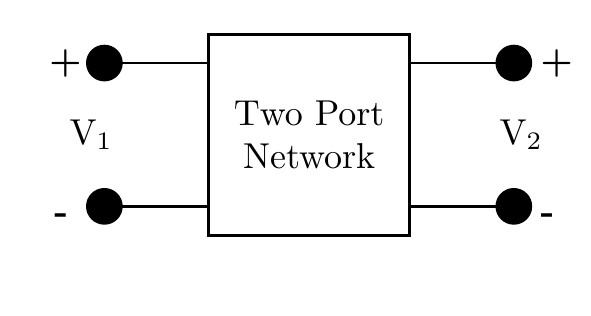
\begin{tikzpicture}[scale=1.3, transform shape]
        % Paths, nodes and wires:
        \node[shape=rectangle, draw, line width=1pt, minimum width=1.965cm, minimum height=1.965cm] at (-0, 1){} node[anchor=center, align=center, text width=1.577cm, inner sep=6pt] at (0, 1){Two Port Network};
        \draw[line width=1pt] (1, 0.3) -- (2, 0.3);
        \draw[line width=1pt] (1, 1.7) -- (2, 1.7);
        \draw[line width=1pt] (-1, 1.7) -- (-2, 1.7);
        \draw[line width=1pt] (-1, 0.3) |- (-2, 0.3);
        \node[shape=circle, fill={rgb,255:red,0;green,0;blue,0}, draw, line width=1pt, minimum width=0.165cm] at (-2, 1.7){};
        \node[shape=circle, fill={rgb,255:red,0;green,0;blue,0}, draw, line width=1pt, minimum width=0.165cm] at (-2, 0.3){};
        \node[shape=circle, fill={rgb,255:red,0;green,0;blue,0}, draw, line width=1pt, minimum width=0.165cm] at (2, 0.3){};
        \node[shape=circle, fill={rgb,255:red,0;green,0;blue,0}, draw, line width=1pt, minimum width=0.165cm] at (2, 1.7){};
        \node[shape=rectangle, minimum width=0.265cm, minimum height=0.265cm] at (-2.35, 1.7){} node[anchor=center, align=center, text width=-0.123cm, inner sep=6pt] at (-2.6, 1.7){\textbf{+}};
        \node[shape=rectangle, minimum width=0.265cm, minimum height=0.265cm] at (2.35, 1.7){} node[anchor=center, align=center, text width=-0.123cm, inner sep=6pt] at (2.2, 1.7){\textbf{+}};
        \node[shape=rectangle, minimum width=0.265cm, minimum height=0.265cm] at (2.35, 0.3){} node[anchor=center, align=center, text width=-0.123cm, inner sep=6pt] at (2.2, 0.0){\textbf{-}};
        \node[shape=rectangle, minimum width=0.265cm, minimum height=0.265cm] at (-2.35, 0.2){} node[anchor=center, align=center, text width=-0.123cm, inner sep=6pt] at (-2.55, 0.0){\textbf{-}};
        \node[shape=rectangle, minimum width=0.615cm, minimum height=0.665cm] at (-2.225, 1){} node[anchor=center, align=center, text width=0.227cm, inner sep=6pt] at (-2.225, 1){$\mathrm{V_1}$};
        \node[shape=rectangle, minimum width=0.615cm, minimum height=0.665cm] at (1.975, 1){} node[anchor=center, align=center, text width=0.227cm, inner sep=6pt] at (1.975, 1){$\mathrm{V_2}$};
    \end{tikzpicture}
    \caption{Two-port network representation}\label{fig:two_port_network}
\end{figure}

At the high frequencies relevant to multi-gigabit serial links, it is often more convenient to describe such a network in terms of traveling waves rather than voltages and currents directly. Scattering parameters (S-parameters) provide this alternative description, characterizing the behavior of a network in terms of the incident and reflected waves present at each of its ports. For a given network, the relationship between the incident and reflected waves at each port can be fully described by an S-parameter matrix.
Figure~\ref{fig:s_parameter_representation} shows the incident and reflected traveling waves used to describe a two-port network.

\begin{figure}[H]
    \centering
    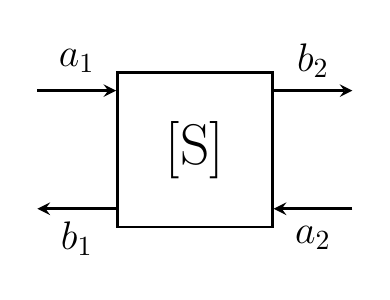
\begin{tikzpicture}[transform shape]
        % Paths, nodes and wires:
        \node[shape=rectangle, draw, line width=1pt, minimum width=1.965cm, minimum height=1.965cm] at (0, -0){} node[anchor=center, align=center, text width=1.577cm, inner sep=6pt] at (0, -0){\huge [S]};
        \draw[line width=1pt, -stealth] (-2, 0.75) -- (-1, 0.75);
        \draw[line width=1pt, -stealth] (1, 0.75) -- (2, 0.75);
        \draw[line width=1pt, -stealth] (2, -0.75) -- (1, -0.75);
        \draw[line width=1pt, -stealth] (-1, -0.75) -- (-2, -0.75);
        \node[shape=rectangle, minimum width=1.215cm, minimum height=0.715cm] at (-1.5, 1.125){} node[anchor=center, align=center, text width=0.827cm, inner sep=6pt] at (-1.5, 1.125){\Large $a_1$};
        \node[shape=rectangle, minimum width=1.215cm, minimum height=0.715cm] at (-1.5, -1.125){} node[anchor=center, align=center, text width=0.827cm, inner sep=6pt] at (-1.5, -1.125){\Large $b_1$};
        \node[shape=rectangle, minimum width=1.215cm, minimum height=0.715cm] at (1.5, -1.125){} node[anchor=center, align=center, text width=0.827cm, inner sep=6pt] at (1.5, -1.125){\Large $a_2$};
        \node[shape=rectangle, minimum width=1.215cm, minimum height=0.715cm] at (1.5, 1.125){} node[anchor=center, align=center, text width=0.827cm, inner sep=6pt] at (1.5, 1.125){\Large $b_2$};
    \end{tikzpicture}
    \caption{S-parameter representation of a two-port network}\label{fig:s_parameter_representation}
\end{figure}

% add S-parameter matrix equation
\[
\begin{bmatrix}
    b_1 \\
    b_2
\end{bmatrix}
=
\begin{bmatrix}
    S_{11} & S_{12} \\
    S_{21} & S_{22}
\end{bmatrix}
\cdot
\begin{bmatrix}
    a_1 \\
    a_2
\end{bmatrix}
\]

For a two-port network, such as a transmission line or channel segment, four S-parameters are defined: 
% transformar em bullet points para facilitar leitura  

\begin{itemize}
    \item $S_{11}$: Input reflection coefficient, describing the fraction of the wave incident at the input port that is reflected back toward the source
    \item $S_{21}$: Forward transmission coefficient, describing the fraction of the incident wave at the input port that is transmitted through the network to the output port
    \item $S_{12}$: Reverse transmission coefficient, describing the fraction of the wave incident at the output port that is transmitted back through the network to the input port
    \item $S_{22}$: Output reflection coefficient, describing the fraction of the wave incident at the output port that is reflected back toward the load
\end{itemize}

% add imagem mostrando reflexoes no N-port

Together, these four coefficients provide a complete characterization of a two-port channel's frequency response, capturing both its insertion loss, primarily reflected in $S_{21}$, and its return loss, primarily reflected in $S_{11}$ and $S_{22}$, as discussed in Sections~\ref{sec:insertion_loss} and \ref{sec:return_loss}.

\subsection{Signal Integrity Metrics}

\subsubsection{Eye Diagram}\label{sec:eye_diagram}

An eye diagram is a graphical representation of a digital signal's voltage as a function of time, constructed by overlaying multiple \acp{UI} of the signal onto a single common time axis. The resulting pattern resembles an open eye, with the open region at its center representing the ideal sampling window available to the \ac{RX}. Eye diagrams provide a compact and visually intuitive means of assessing \ac{SI}~\cite{bogatin_SI}, since they reveal several critical \ac{SI} parameters simultaneously, including an estimate of \ac{BER}, \ac{SNR}, and the available timing and voltage margins.
The construction of an eye diagram from overlapping signal intervals is illustrated in Figure~\ref{fig:eye_diagram_example}.

\begin{figure}[H]
    \centering
    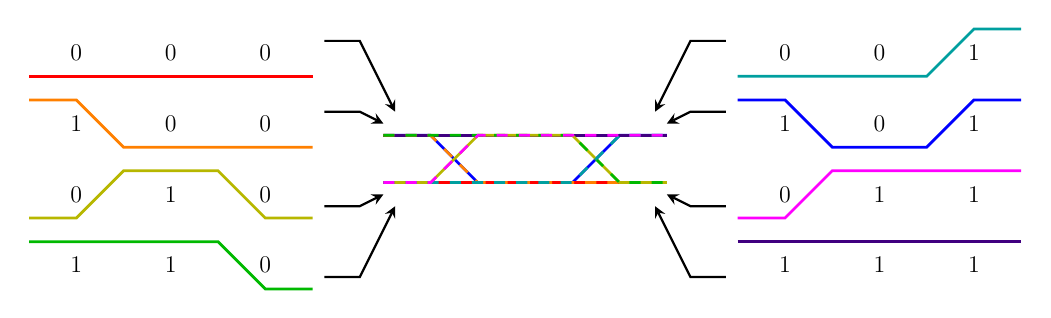
\begin{tikzpicture}[scale=0.6, transform shape]
        % Paths, nodes and wires:
        \path[draw={rgb,255:red,0;green,0;blue,255}, line width=1pt] (-3, 3.25) -- (-2, 3.25) -- (-1, 2.25) -- (1, 2.25) -- (2, 3.25) -- (3, 3.25);
        \path[draw={rgb,255:red,255;green,0;blue,0}, line width=1pt] (-10.5, 4.5) -- (-4.5, 4.5);
        \path[draw={rgb,255:red,255;green,128;blue,0}, line width=1pt] (-10.5, 4) -- (-9.5, 4) -- (-8.5, 3) -- (-4.5, 3);
        \path[draw={rgb,255:red,183;green,183;blue,0}, line width=1pt] (-10.5, 1.5) -- (-9.5, 1.5) -- (-8.5, 2.5) -- (-6.5, 2.5) -- (-5.5, 1.5) -- (-4.5, 1.5);
        \path[draw={rgb,255:red,0;green,185;blue,0}, line width=1pt] (-10.5, 1) -- (-6.5, 1) -- (-5.5, -0) -- (-4.5, -0);
        \path[draw={rgb,255:red,0;green,159;blue,159}, line width=1pt] (4.5, 4.5) -- (8.5, 4.5) -- (9.5, 5.5) -- (10.5, 5.5);
        \path[draw={rgb,255:red,0;green,0;blue,255}, line width=1pt] (4.5, 4) -- (5.5, 4) -- (6.5, 3) -- (8.5, 3) -- (9.5, 4) -- (10.5, 4);
        \path[draw={rgb,255:red,255;green,0;blue,255}, line width=1pt] (4.5, 1.5) -- (5.5, 1.5) -- (6.5, 2.5) -- (10.5, 2.5);
        \path[draw={rgb,255:red,64;green,0;blue,128}, line width=1pt] (4.5, 1) -- (10.5, 1);
        \node[shape=rectangle, minimum width=0.965cm, minimum height=0.965cm] at (-9.5, 5){} node[anchor=center, align=center, text width=0.577cm, inner sep=6pt] at (-9.5, 5){\Large 0};
        \node[shape=rectangle, minimum width=0.965cm, minimum height=0.965cm] at (-7.5, 5){} node[anchor=center, align=center, text width=0.577cm, inner sep=6pt] at (-7.5, 5){\Large 0};
        \node[shape=rectangle, minimum width=0.965cm, minimum height=0.965cm] at (-5.5, 5){} node[anchor=center, align=center, text width=0.577cm, inner sep=6pt] at (-5.5, 5){\Large 0};
        \node[shape=rectangle, minimum width=0.965cm, minimum height=0.965cm] at (-9.5, 3.5){} node[anchor=center, align=center, text width=0.577cm, inner sep=6pt] at (-9.5, 3.5){\Large 1};
        \node[shape=rectangle, minimum width=0.965cm, minimum height=0.965cm] at (-7.5, 3.5){} node[anchor=center, align=center, text width=0.577cm, inner sep=6pt] at (-7.5, 3.5){\Large 0};
        \node[shape=rectangle, minimum width=0.965cm, minimum height=0.965cm] at (-5.5, 3.5){} node[anchor=center, align=center, text width=0.577cm, inner sep=6pt] at (-5.5, 3.5){\Large 0};
        \node[shape=rectangle, minimum width=0.965cm, minimum height=0.965cm] at (-9.5, 2){} node[anchor=center, align=center, text width=0.577cm, inner sep=6pt] at (-9.5, 2){\Large 0};
        \node[shape=rectangle, minimum width=0.965cm, minimum height=0.965cm] at (-7.5, 2){} node[anchor=center, align=center, text width=0.577cm, inner sep=6pt] at (-7.5, 2){\Large 1};
        \node[shape=rectangle, minimum width=0.965cm, minimum height=0.965cm] at (-5.5, 2){} node[anchor=center, align=center, text width=0.577cm, inner sep=6pt] at (-5.5, 2){\Large 0};
        \node[shape=rectangle, minimum width=0.965cm, minimum height=0.965cm] at (-9.5, 0.5){} node[anchor=center, align=center, text width=0.577cm, inner sep=6pt] at (-9.5, 0.5){\Large 1};
        \node[shape=rectangle, minimum width=0.965cm, minimum height=0.965cm] at (-7.5, 0.5){} node[anchor=center, align=center, text width=0.577cm, inner sep=6pt] at (-7.5, 0.5){\Large 1};
        \node[shape=rectangle, minimum width=0.965cm, minimum height=0.965cm] at (-5.5, 0.5){} node[anchor=center, align=center, text width=0.577cm, inner sep=6pt] at (-5.5, 0.5){\Large 0};
        \node[shape=rectangle, minimum width=0.965cm, minimum height=0.965cm] at (5.5, 5){} node[anchor=center, align=center, text width=0.577cm, inner sep=6pt] at (5.5, 5){\Large 0};
        \node[shape=rectangle, minimum width=0.965cm, minimum height=0.965cm] at (7.5, 5){} node[anchor=center, align=center, text width=0.577cm, inner sep=6pt] at (7.5, 5){\Large 0};
        \node[shape=rectangle, minimum width=0.965cm, minimum height=0.965cm] at (9.5, 5){} node[anchor=center, align=center, text width=0.577cm, inner sep=6pt] at (9.5, 5){\Large 1};
        \node[shape=rectangle, minimum width=0.965cm, minimum height=0.965cm] at (5.5, 3.5){} node[anchor=center, align=center, text width=0.577cm, inner sep=6pt] at (5.5, 3.5){\Large 1};
        \node[shape=rectangle, minimum width=0.965cm, minimum height=0.965cm] at (7.5, 3.5){} node[anchor=center, align=center, text width=0.577cm, inner sep=6pt] at (7.5, 3.5){\Large 0};
        \node[shape=rectangle, minimum width=0.965cm, minimum height=0.965cm] at (9.5, 3.5){} node[anchor=center, align=center, text width=0.577cm, inner sep=6pt] at (9.5, 3.5){\Large 1};
        \node[shape=rectangle, minimum width=0.965cm, minimum height=0.965cm] at (5.5, 2){} node[anchor=center, align=center, text width=0.577cm, inner sep=6pt] at (5.5, 2){\Large 0};
        \node[shape=rectangle, minimum width=0.965cm, minimum height=0.965cm] at (7.5, 2){} node[anchor=center, align=center, text width=0.577cm, inner sep=6pt] at (7.5, 2){\Large 1};
        \node[shape=rectangle, minimum width=0.965cm, minimum height=0.965cm] at (9.5, 2){} node[anchor=center, align=center, text width=0.577cm, inner sep=6pt] at (9.5, 2){\Large 1};
        \node[shape=rectangle, minimum width=0.965cm, minimum height=0.965cm] at (5.5, 0.5){} node[anchor=center, align=center, text width=0.577cm, inner sep=6pt] at (5.5, 0.5){\Large 1};
        \node[shape=rectangle, minimum width=0.965cm, minimum height=0.965cm] at (7.5, 0.5){} node[anchor=center, align=center, text width=0.577cm, inner sep=6pt] at (7.5, 0.5){\Large 1};
        \node[shape=rectangle, minimum width=0.965cm, minimum height=0.965cm] at (9.5, 0.5){} node[anchor=center, align=center, text width=0.577cm, inner sep=6pt] at (9.5, 0.5){\Large 1};
        \path[draw={rgb,255:red,255;green,0;blue,0}, line width=1pt] (-3, 2.25) -- (3, 2.25);
        \path[draw={rgb,255:red,64;green,0;blue,128}, line width=1pt] (-3, 3.25) -- (3, 3.25);
        \path[draw={rgb,255:red,255;green,128;blue,0}, line width=1pt, dash pattern={on 4pt off 4pt}] (-3, 3.25) -- (-2, 3.25) -- (-1, 2.25) -- (3, 2.25);
        \path[draw={rgb,255:red,183;green,183;blue,0}, line width=1pt] (-3, 2.25) -- (-2, 2.25) -- (-1, 3.25) -- (1, 3.25) -- (2, 2.25) -- (3, 2.25);
        \path[draw={rgb,255:red,0;green,185;blue,0}, line width=1pt, dash pattern={on 4pt off 4pt}] (-3, 3.25) -- (1, 3.25) -- (2, 2.25) -- (3, 2.25);
        \path[draw={rgb,255:red,0;green,159;blue,159}, line width=1pt, dash pattern={on 4pt off 4pt}] (-3, 2.25) -- (1, 2.25) -- (2, 3.25) -- (3, 3.25);
        \path[draw={rgb,255:red,255;green,0;blue,255}, line width=1pt, dash pattern={on 4pt off 4pt}] (-3, 2.25) -- (-2, 2.25) -- (-1, 3.25) -- (3, 3.25);
        \draw[line width=0.8pt, -stealth] (-4.25, 5.25) -- (-3.5, 5.25) -- (-2.75, 3.75);
        \draw[line width=0.8pt, -stealth] (-4.25, 3.75) -- (-3.5, 3.75) -- (-3, 3.5);
        \draw[line width=0.8pt, -stealth] (-4.25, 0.25) -- (-3.5, 0.25) -- (-2.75, 1.75);
        \draw[line width=0.8pt, -stealth] (-4.25, 1.75) -- (-3.5, 1.75) -- (-3, 2);
        \draw[line width=0.8pt, -stealth] (4.25, 0.25) -- (3.5, 0.25) -- (2.75, 1.75);
        \draw[line width=0.8pt, -stealth] (4.25, 1.75) -- (3.5, 1.75) -- (3, 2);
        \draw[line width=0.8pt, -stealth] (4.25, 5.25) -- (3.5, 5.25) -- (2.75, 3.75);
        \draw[line width=0.8pt, -stealth] (4.25, 3.75) -- (3.5, 3.75) -- (3, 3.5);
        \end{tikzpicture}
        \caption{Eye diagram construction}\label{fig:eye_diagram_example}
\end{figure}

These metrics can be extracted directly from the geometry of the eye diagram, by analyzing its vertical and horizontal openings, as well as the shape and symmetry of the signal transitions that form its boundaries. 

The horizontal opening, or width, of the eye indicates the timing margin available for reliable sampling, that is, the duration for which the signal remains valid around the ideal sampling instant. Jitter can be estimated by analyzing the degree of closure of this horizontal opening. 

The vertical opening, or height, of the eye indicates the voltage difference between the lowest observed logical-high level and the highest observed logical-low level; it reflects the overall clarity of the signal, with its size directly related to the noise present in the system and the resulting \ac{SNR}, and is strongly correlated with the achievable \ac{BER}.

\begin{comment}
\begin{figure}
    \centering
    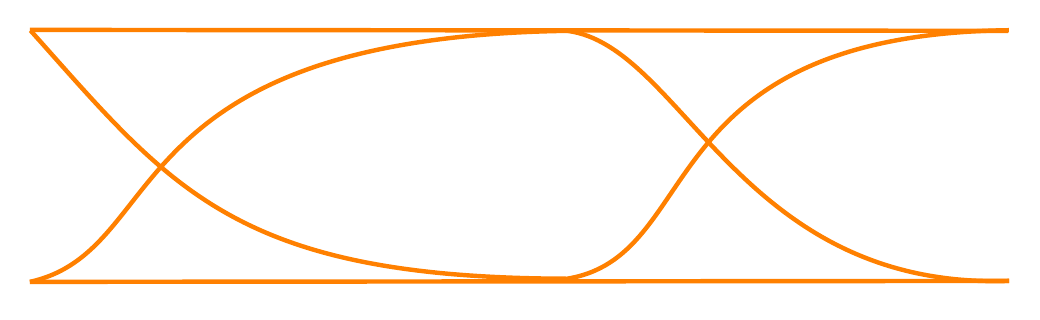
\begin{tikzpicture}[scale=0.4]
        % Coordinates
        \coordinate (A) at (0.00, 0.00);
        \coordinate (B) at (31.09, 0.03);
        \coordinate (C) at (-0.00, 8.00);
        \coordinate (D) at (31.06, 7.97);
        \coordinate (E) at (17.06, 7.97);
        \coordinate (F) at (4.50, 1.00);
        \coordinate (G) at (2.50, 7.75);
        \coordinate (H) at (20.75, 7.50);
        \coordinate (I) at (22.50, -0.25);
        \coordinate (J) at (0.02, 7.98);
        \coordinate (K) at (4.47, 3.01);
        \coordinate (L) at (6.46, 0.13);
        \coordinate (M) at (17.01, 0.10);
        \coordinate (N) at (16.99, 0.09);
        \coordinate (O) at (21.50, 0.75);
        \coordinate (P) at (19.49, 7.84);
        \coordinate (Q) at (31.08, 7.99);

        % Drawing
        \draw[orange, ultra thick] (A) -- (B);
        \draw[orange, ultra thick] (C) -- (D);
        \draw[orange, ultra thick] (A) .. controls (4.50, 1.00) and (2.50, 7.75) .. (E);
        \draw[orange, ultra thick] (E) .. controls (20.75, 7.50) and (22.50, -0.25) .. (B);
        \draw[orange, ultra thick] (J) .. controls (4.47, 3.01) and (6.46, 0.13) .. (M);
        \draw[orange, ultra thick] (N) .. controls (21.50, 0.75) and (19.49, 7.84) .. (Q);
    \end{tikzpicture}
    \caption{Eye diagram with horizontal and vertical openings}\label{fig:eye_diagram_openings}
\end{figure}
\end{comment}

The leading and trailing edges of the eye diagram correspond to the rising and falling transitions of the signal between bit periods. The region where these transitions cross one another, near the edges of the eye, highlights the variation present across individual bit transitions, providing a visual indication of the total jitter affecting the signal and its impact on overall signal quality.

Eye amplitude refers to the peak-to-peak voltage of the signal, defining the full voltage swing between a logical `1' and a logical `0'. For an ideal, undistorted signal, the eye amplitude and eye height are approximately equal; however, insertion loss and other channel impairments often cause a noticeable reduction in eye height relative to the nominal transmitted amplitude, as energy from the signal is lost or redistributed into neighboring symbols.

An eye mask defines a predefined keep-out region within the eye diagram, specifying the minimum acceptable eye opening required for compliance with a given standard. Any portion of the received signal that falls within this keep-out region constitutes an eye mask violation, indicating non-compliant signal integrity.

Rise and fall times define the speed at which the signal transitions between its two voltage levels, its slew rate. Excessively slow transitions blur the contour of the eye diagram and reduce the clarity of the resulting eye opening. The threshold, or crossing percentage, refers to the signal level at which a receiver can reliably distinguish between a logical `1' and a logical `0' while maintaining an acceptable \ac{BER}, and defines the effective decision point used when interpreting the eye diagram.

Taken together, eye diagrams allow several distinct signal integrity impairments, including insertion loss, \ac{ISI}, crosstalk, reflections and impedance mismatches, and jitter and timing errors, to be identified and, to some extent, distinguished from one another through visual inspection of the resulting eye shape.
    
\section{Equalization}\label{sec:equalization}
    
Equalization is a signal-processing technique in which the transmitted data signal is deliberately distorted using a transform that approximates the inverse of the channel's frequency response. The goal of equalization is to flatten the overall frequency response of the \ac{TX}-channel-receiver system out to the Nyquist frequency, discussed in Section~\ref{sec:nrz_encoding}, thereby removing, or substantially reducing, the time-domain \ac{ISI} introduced by the channel~\cite{zamir2018_nrz_pam4,sredojevic_jssc_2011}, as described in Section~\ref{sec:isi_detailed}. Equalization can, in principle, be implemented at the \ac{TX}, at the \ac{RX}, or split between both, depending on the specific link architecture and standard requirements.
The frequency-dependent attenuation that motivates equalization is illustrated in Figure~\ref{fig:eq_channel_response}.

\begin{figure}[h]
    \centering
    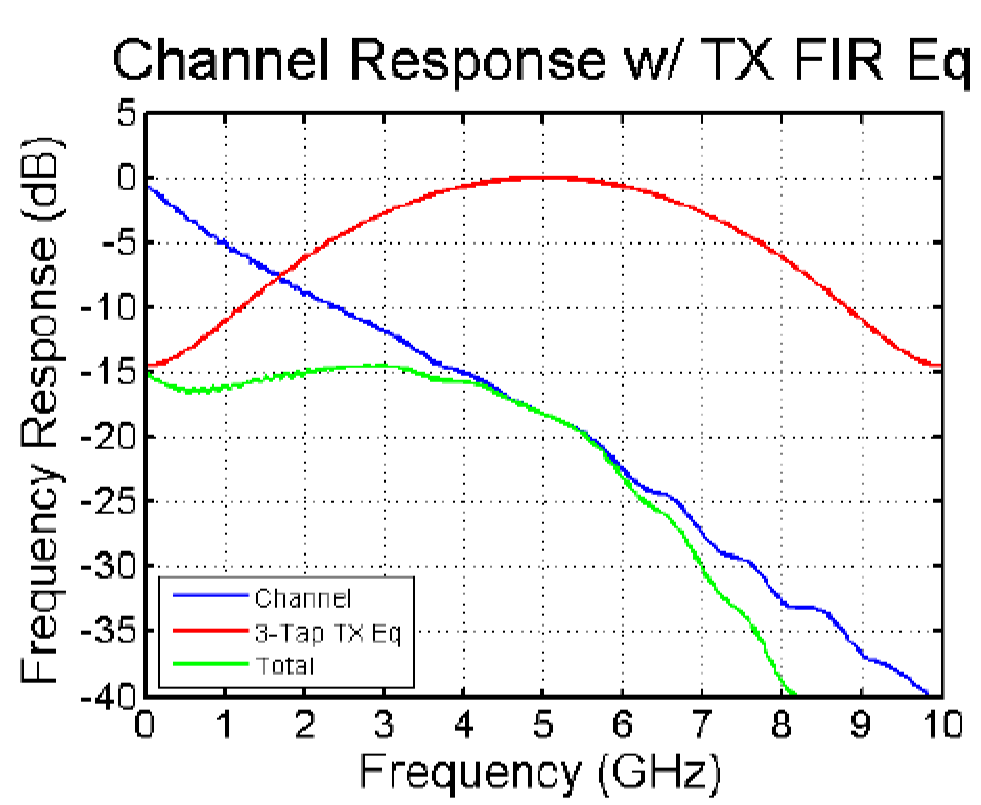
\includegraphics[width=0.6\textwidth]{figures/chapter2/EQ_channel_response_palermo_ecen720_lab5.png}
    \caption{Channel response. Reproduced from \cite{palermo_ecen720_lab5}}\label{fig:eq_channel_response}
\end{figure}

As discussed in Section~\ref{sec:insertion_loss}, practical electrical channels typically exhibit progressively greater loss at higher frequencies. This behavior is particularly problematic for high-speed serial links, since the high-frequency spectral components of the transmitted signal are primarily responsible for producing sharp signal transitions and, consequently, for determining the eye opening observed at the receiver. Equalization is therefore used specifically to compensate for these high-frequency losses, restoring the spectral balance of the signal and preserving adequate eye opening at the sampling point.

    %MOSTRAR EYE DIAGRAM - BIT TRANSITIONS CARRY THE HIGH FREQ COMPONENTS OF THE SIGNAL - WHEN ANALYZING BOTH LEADING AND TRAILING EDGES OF THE EYE, THEY REVEAL HOW DIFFERENT EQ TECHNIQUES INFLUENCE SI

    %https://www.protoexpress.com/blog/analyzing-eye-diagrams-for-signal-integrity-high-speed-pcbs/
 
\subsection{Transmitter-Side Equalization}\label{sec:tx_side_equalization}

\ac{TX}-side equalization operates by pre-distorting the transmitted signal in a manner designed to invert the anticipated distortion introduced by the channel~\cite{chen_tx_equalizer_2009,zamir2018_nrz_pam4}, a technique commonly referred to as transmit pre-emphasis. In practice, since the overall signal swing available at the \ac{TX} is bounded, this pre-distortion is realized by selectively boosting the high-frequency transitions of the signal relative to its low-frequency, steady-state content; the practical effect of this boosting, given a fixed total output swing, is an attenuation of the steady-state levels of the transmitted signal relative to its transition levels, in order to compensate for the high-frequency losses introduced by the channel, as discussed in the context of \ac{PS} and \ac{DE} in Section~\ref{sec:tx_equalization}.

The distortion intentionally introduced at the \ac{TX} is subsequently reverted, at least in part, at the receiver, through \ac{RX}-side equalization techniques such as \ac{CTLE} or \ac{DFE}, which further shape the received signal to restore an adequately open eye at the sampling point~\cite{zamir2018_nrz_pam4}.

\ac{TX}-side equalization is most commonly implemented using a multi-tap \ac{FIR} structure, referred to as \ac{FFE}. This \ac{FIR} structure operates by applying a set of delayed and scaled copies of the original signal, and combining them with the original signal using an appropriate set of weights~\cite{chen_tx_equalizer_2009,sredojevic_jssc_2011}, or tap coefficients.

This weighted combination is performed specifically to counteract the effects of \ac{ISI} caused by channel dispersion~\cite{zamir2018_nrz_pam4}: since a dispersive channel spreads the energy of each transmitted symbol into neighboring unit intervals, as discussed in Section~\ref{sec:isi_detailed}, the \ac{FFE} pre-compensates for this effect by effectively adding the anticipated dispersed portion of a symbol's energy back into the signal ahead of time, at the \ac{TX}, rather than allowing it to be lost to the channel's frequency response.

For Gen 2 operation, the \ac{USB} 3.2 specification defines a three-tap \ac{FIR} filter structure for the \ac{TX} equalizer.

\subsubsection{\acs*{FFE} and the 3-Tap \acs*{FIR} Architecture} %REVER - CONTEUDO DA SUBSECAO ANTERIOR REPETIDO 

High-speed serial links such as \ac{USB} 3.2 transmit data over channels that behave as low-pass filters, attenuating the high-frequency content of the signal far more than its low-frequency content. As the transmitted bit rate increases, the channel's limited bandwidth causes each pulse, resulting in \ac{ISI} and a closed eye diagram at the \ac{RX} and severely limits the maximum achievable data rate. Equalization is the general technique used to counteract this effect, either at the receiver, at the \ac{TX}, or through a combination of both.
The three-tap \ac{FIR} architecture, with precursor, main, and postcursor coefficients, is shown in Figure~\ref{fig:3_tap_FIR_EQ}.

\ac{FFE} is one of the principal techniques used to combat \ac{ISI}, and can be implemented at either end of the link. Conceptually, an \ac{FFE} stage generates a number of delayed copies of the input signal, scales each copy by a weighting coefficient, and sums the results to produce the equalized output. An \ac{FFE} implementation looks for all intents and purposes like a digital \ac{FIR} filter. When applied at the \ac{TX}, this process is commonly referred to as pre-empahsis or de-emphasis, and is implemented directly in the driver by scaling the current, and hence the voltage swing, associated with each delayed version of the data.

\begin{figure}[H]

    \centering
    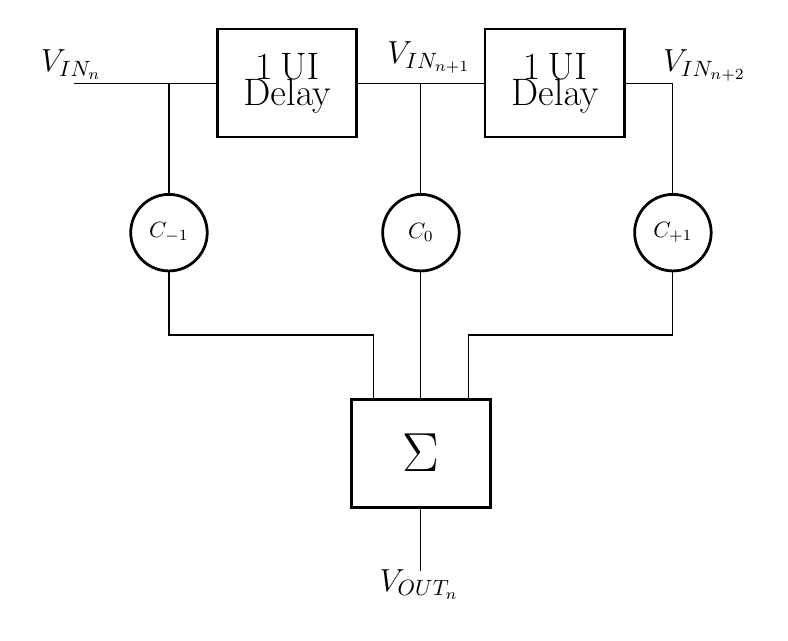
\begin{tikzpicture}[scale=0.8, transform shape]
    % Paths, nodes and wires:
    \node[shape=rectangle, draw, line width=1pt, minimum width=2.215cm, minimum height=1.715cm] at (11.875, 14){} node[anchor=center, align=center, text width=1.827cm, inner sep=6pt] at (11.875, 14){\LARGE 1 UI\\Delay};
    \node[shape=circle, draw, line width=1pt, minimum width=1.215cm](N1) at (10, 11.625){} node[anchor=center] at (N1.text){$C_{-1}$};
    \node[shape=circle, draw, line width=1pt, minimum width=1.215cm](N2) at (14, 11.625){} node[anchor=center] at (N2.text){$C_{0}$};
    \node[shape=circle, draw, line width=1pt, minimum width=1.215cm](N3) at (18, 11.625){} node[anchor=center] at (N3.text){$C_{+1}$};
    \node[shape=rectangle, draw, line width=1pt, minimum width=2.215cm, minimum height=1.715cm] at (16.125, 14){} node[anchor=center, align=center, text width=1.827cm, inner sep=6pt] at (16.125, 14){\LARGE 1 UI\\Delay};
    \draw (10.75, 14) -- (8.5, 14);
    \draw (13, 14) -- (15, 14);
    \draw (17.25, 14) -- (18, 14);
    \node[shape=rectangle, draw, line width=1pt, minimum width=2.215cm, minimum height=1.715cm] at (14, 8.125){} node[anchor=center, align=center, text width=1.827cm, inner sep=6pt] at (14, 8.125){\Huge $\Sigma$};
    \draw (10, 12.25) -- (10, 14);
    \draw (14, 12.25) -| (14, 14);
    \draw (18, 12.25) -| (18, 14);
    \draw (14, 11) -- (14, 10);
    \draw (14, 9) -| (14, 10);
    \draw (13.25, 9) -| (13.25, 10) -| (10, 10.25) -| (10, 11);
    \draw (14.75, 9) -| (14.75, 10) -- (18, 10) -| (18, 11);
    \draw (14, 7.25) -| (14, 6.25);
    \node[shape=rectangle, minimum width=1.715cm, minimum height=0.465cm] at (8.625, 14.5){} node[anchor=north west, align=left, text width=1.327cm, inner sep=6pt] at (7.75, 14.75){\Large $V_{IN_{n}}$};
    \node[shape=rectangle, minimum width=1.715cm, minimum height=0.465cm] at (14.125, 14.625){} node[anchor=north west, align=left, text width=1.327cm, inner sep=6pt] at (13.25, 14.875){\Large $V_{IN_{n+1}}$};
    \node[shape=rectangle, minimum width=1.715cm, minimum height=0.465cm] at (18.5, 14.5){} node[anchor=north west, align=left, text width=1.327cm, inner sep=6pt] at (17.625, 14.75){\Large $V_{IN_{n+2}}$};
    \node[shape=rectangle, minimum width=1.715cm, minimum height=0.465cm] at (14, 6.25){} node[anchor=north west, align=left, text width=1.327cm, inner sep=6pt] at (13.125, 6.5){\Large $V_{OUT_{n}}$};
    \end{tikzpicture}

\caption{3-tap \ac{TX} Equalizer Structure}\label{fig:3_tap_FIR_EQ}
\end{figure}

Because the \ac{FFE} structure is functionally a \ac{FIR} filter, its behaviour can be described using the standard discrete-time convolution sum~\cite{chen_tx_equalizer_2009}. For a filter with $N$ taps and coefficients $c_k$, the equalized output sample $y[n]$ is given by

\begin{equation}
y[n] = \sum_{k=-M}^{P} c_k \, x[n-k]
\label{eq:fir_general}
\end{equation}

where $x[n]$ is the input data sequence, $M$ is the number of post-cursor taps and $P$ is the number of pre-cursor taps. Each tap introduces a delay of one \ac{UI} relative to its neighbour, so that the filter effectively looks both ahead of and behind the current symbol being transmitted \ac{FFE} creates a number of delayed versions of the input signal that are added back to the signal with the proper weights. Typically, the delay is 1 \ac{UI} in duration.

%[REMOVER - VER COMENTARIO DO DENIS DRAFT 3]In practice, \ac{TX}-side FFE implementations are rarely built with more than a handful of taps, since each additional tap adds delay elements, current sources, and control complexity to the driver without providing a proportional improvement in equalization performance for typical channel lengths [REF]. Typically, the FIR filters used to perform \ac{TX} pre-emphasis are three-tap filters, and this is the architecture adopted for the driver described in this work. 

The \ac{FIR} structure proposed by the \ac{USB} 3.2 specification is a 3-tap filter.In this structure, three consecutive symbols in the data stream are each scaled by their own coefficient and summed to produce the driver output for the current symbol. Denoting the coefficients as $c_{-1}$, $c_0$ and $c_1$, Equation~\eqref{eq:fir_general} reduces to

\begin{equation}
y[n] = c_{-1}\,x[n+1] + c_0\,x[n] + c_1\,x[n-1]
\label{eq:fir_3tap}
\end{equation}

Each of the three taps plays a distinct role in shaping the transmitted waveform. One tap handles pre-cursor ISI, one post-cursor ISI, and one current-cursor ISI.  The main, or cursor, tap $c_0$ operates on the symbol currently being transmitted and is responsible for setting the nominal output swing of the driver. The pre-cursor tap $c_{-1}$ operates on the symbol that has not yet been transmitted, and is used to boost or attenuate the leading edge of the current symbol in anticipation of teh transition that follows~\cite{chen_tx_equalizer_2009}; this is the mechanism responsible for the preshoot behaviour introduced earlier in this section. The post-cursor tap $c_1$ operates on the previously transmitted symbol, and is used to cancel the residual energy left behind by that symbol's transition~\cite{chen_tx_equalizer_2009,zamir2018_nrz_pam4}; this is the mechanism responsible for de-emphasis. Because the taps act on immediately adjacent symbols, the polarity of $c_{-1}$ and $c_1$ relative to $c_0$ depends on whether consecutive symbols represent a transition or a repeated bit, which is what allows the filter to selectively boost transition edges while leaving steady-state levels comparatively unaffected.

A defining property of this class of equalizer is that the total weight distributed across the taps is fixed, so that increasing the magnitude of the pre- and post-cursor taps necessarily reduces the magnitude of the main tap, and vice versa. This behaviour is captured by the normalization constraint introduced later in this section (Equation~\eqref{eq:tap_constraint}), and reflects a fundamental trade-off in \ac{FFE} design: stronger equalization sharpens transition edges and opens the eye at the receiver, but does so at the cost of a reduced main-tap amplitude and, consequently, reduced overall signal swing. 

\section{Transmitter Drivers} \label{sec:tx_drivers_background}

Data generated by digital circuitry, such as the serialized bitstream produced by a serializer, is typically represented as voltage levels corresponding to binary logic states. These voltage levels, together with the digital encoding scheme used to represent them, are generally not directly suitable for transmission over a physical channel, due to limitations in \ac{SI}, power efficiency, and compatibility with the electrical characteristics of the channel itself. The \ac{TX} driver serves as the interface between the digital logic domain and the physical transmission medium, converting the digital logic signal into an analog waveform that can be reliably transmitted over the channel while meeting the required \ac{SI} and power efficiency specifications~\cite{zamir2018_nrz_pam4}.

Beyond this basic conversion function, the \ac{TX} driver is also responsible for modifying the transmitted signal to compensate for channel losses, through equalization techniques that account for the frequency-dependent attenuation and dispersion introduced by the channel~\cite{chen_cml_review_2026,zamir2018_nrz_pam4}, as discussed in Section~\ref{sec:equalization}. This pre-distortion of the transmitted waveform enables the \ac{RX} to correctly interpret the received signal and recover the original data with minimal errors, despite the non-ideal frequency response of the channel.

As data rates increase, the performance margins within which the \ac{TX} driver must operate become significantly tighter. Higher data rates demand faster rise and fall times, lower \ac{TX}-generated jitter, higher driver bandwidth, and more stringent control over \ac{SI} metrics such as eye opening and \ac{BER}. In addition to these speed-related requirements, it is generally desirable for the \ac{TX} driver to be designed for low power consumption, since power efficiency is a key design constraint in most modern high-speed serial interfaces.

\subsection{Driver Architectures} \label{sec:tx_driver_architectures}

%A driver's output signaling can be performed with two primary methods, voltage and current-mode. Voltage-mode based drivers acts as a voltage source to drive a signal to the load, while current-mode drivers act as a controlled current source. 

The two principal controlled-impedance driver architectures can be represented by the simplified functional models shown in Figure~\ref{fig:driver_functional}. A current-mode driver uses a controlled current source together with a parallel termination and is therefore analogous to a Norton source, whereas a voltage-mode driver uses a low-impedance voltage source together with series termination and is analogous to a Thévenin source.


\begin{figure}[H]
    \centering
    \begin{subfigure}{0.4\textwidth}
        \centering
        \resizebox{\linewidth}{!}{
        \begin{tikzpicture}[transform shape]
            % Paths, nodes and wires:
            \node[tlinestub](N1) at (1.125, 4.031){} node[anchor=south] at (N1.text){$Z_0$};
            \draw (0.375, 4.031) to[opening switch] (0.375, 3.031);
            \node[tlinestub] at (1.25, 2.656){};
            \draw (5.375, 4.031) to[american resistor, /tikz/circuitikz/bipoles/length=1.05cm, l={$R$}] (5.375, 5.656);
            \draw[line width=0.8pt, dash pattern={on 3.2pt off 3.2pt}] (4.375, 2.656) -- (5.625, 2.656);
            \node[shape=rectangle, minimum width=1.465cm, minimum height=0.965cm] at (6.375, 3.281){} node[anchor=center, align=center, text width=1.077cm, inner sep=6pt] at (6.375, 3.281){\small $V_{diff}$};
            \node[shape=rectangle, minimum width=0.34cm, minimum height=0.277cm](N2) at (6.875, 4.031){} node[anchor=center] at (N2.text){$+$};
            \node[shape=rectangle, minimum width=0.34cm, minimum height=0.34cm](N3) at (5.875, 2.656){} node[anchor=center] at (N3.text){$-$};
            \node[vee, xscale=-1, yscale=-1] at (5.375, 5.656){};
            \draw[line width=0.8pt, dash pattern={on 3.2pt off 3.2pt}] (5.375, 4.031) -- (6.625, 4.031);
            \draw (-0.625, 2.651) to[closing switch, invert] (-0.625, 1.651);
            \draw[line width=1.1pt, latex-] (1.375, 2.281) -- (2.75, 2.281);
            \node[shape=rectangle, xscale=-1, yscale=-1, minimum width=0.715cm, minimum height=0.465cm](N4) at (2, 2.031){} node[anchor=center] at (N4.center){$I$};
            \draw (1.125, 4.031) to[short, -*] (0.375, 4.031);
            \draw (5.375, 4.031) -- (2.5, 4.031);
            \draw (4.375, 2.656) to[american resistor, /tikz/circuitikz/bipoles/length=1.05cm, l={$R$}] (4.375, 4.281);
            \node[vee, xscale=-1, yscale=-1] at (4.375, 4.281){};
            \draw (4.375, 2.656) -- (2.625, 2.656);
            \draw (1.25, 2.656) to[short, -*] (-0.625, 2.656);
            \draw (0.375, 4.031) to[american resistor, /tikz/circuitikz/bipoles/length=1.05cm, l={$R$}] (0.375, 5.656);
            \node[vee, xscale=-1, yscale=-1] at (0.375, 5.656){};
            \draw (-0.625, 2.656) to[american resistor, /tikz/circuitikz/bipoles/length=1.05cm, l={$R$}] (-0.625, 4.281);
            \node[vee, xscale=-1, yscale=-1] at (-0.625, 4.281){};
            \draw (-0, 2.531) to[american current source, *-, /tikz/circuitikz/bipoles/length=0.952cm, l={$I_{S}$}] (-0, 0.406);
            \draw (-0.625, 1.651) -- (0.375, 3.031);
            \node[vee] at (-0, 0.406){};
        \end{tikzpicture}
        }
    \caption{Current-mode functional model}\label{fig:CM_functional} 
    \end{subfigure}
    \begin{subfigure}{0.49\textwidth}
        \centering
        \resizebox{\linewidth}{!}{
        \begin{tikzpicture}[transform shape]
            % Paths, nodes and wires:
            \node[tlinestub](N1) at (3.85, 2.937){} node[anchor=south] at (N1.text){$Z_0$};
            \draw (2.83, 1.938) to[american resistor, /tikz/circuitikz/bipoles/length=1.05cm, l={$R$}] (1.23, 1.938);
            \draw (3.85, 2.937) to[american resistor, /tikz/circuitikz/bipoles/length=1.05cm, l={$R$}] (2.23, 2.937);
            \draw (2.23, 2.937) to[opening switch] (1.23, 2.937);
            \node[tlinestub] at (3.375, 1.938){};
            \draw (4.75, 1.938) to[short] (5.875, 1.938);
            \draw (5.875, 1.938) to[american resistor, /tikz/circuitikz/bipoles/length=1.05cm, l={$R$}] (5.875, 0.438);
            \draw (6.625, 2.938) to[american resistor, /tikz/circuitikz/bipoles/length=1.05cm, l={$R$}] (6.625, 1.313);
            \draw[line width=0.8pt, dash pattern={on 3.2pt off 3.2pt}] (5.875, 1.938) -- (7.125, 1.938);
            \node[shape=rectangle, minimum width=1.465cm, minimum height=0.965cm] at (7.725, 2.437){} node[anchor=center, align=center, text width=1.077cm, inner sep=6pt] at (7.725, 2.437){\small $V_{diff}$};
            \node[shape=rectangle, minimum width=0.34cm, minimum height=0.277cm] at (8.063, 2.938){} node[anchor=center, align=center, text width=-0.048cm, inner sep=6pt] at (8.063, 2.938){\small +};
            \node[shape=rectangle, minimum width=0.34cm, minimum height=0.34cm] at (7.375, 1.938){} node[anchor=center, align=center, text width=-0.048cm, inner sep=6pt] at (7.375, 1.938){\small -};
            \draw (1.48, 2.687) -- (1.23, 2.687) -- (1.235, 2.687);
            \node[vee] at (1.225, 1.313){};
            \node[vee] at (0.225, 0.437){};
            \node[rground, xscale=-1, yscale=-1](N2) at (1.23, 2.937){} node[anchor=south] at (N2.south){$V_H$};
            \node[rground, xscale=-1, yscale=-1](N3) at (0.23, 1.938){} node[anchor=south] at (N3.south){$V_H$};
            \draw (2.83, 1.938) to[short] (3.475, 1.938);
            \draw (5.225, 2.937) to[short] (6.625, 2.938);
            \node[vee] at (5.875, 0.438){};
            \node[vee] at (6.625, 1.313){};
            \draw (0.22, 0.437) -- (0.22, 1.687);
            \draw (1.225, 1.313) -- (1.225, 2.687);
            \draw (0.47, 1.687) -- (0.22, 1.687) -- (0.225, 1.687);
            \draw[line width=0.8pt, dash pattern={on 3.2pt off 3.2pt}] (6.625, 2.938) -- (7.875, 2.938);
            \draw (1.23, 1.938) to[closing switch] (0.23, 1.938);
            \draw[line width=1.1pt, -latex] (2.625, 1.625) -- (4, 1.625);
            \node[shape=rectangle, minimum width=0.715cm, minimum height=0.465cm](N4) at (3.25, 1.375){} node[anchor=center] at (N4.center){$I$};
        \end{tikzpicture}
        }
    \caption{Voltage-mode functional model}\label{fig:VM_functional}
    \end{subfigure}
    \caption{Differential driver functional models}\label{fig:driver_functional}
\end{figure}

\begin{comment}
    
Both driver architectures can be functionally analyzed using a simplified switch-based model, as shown in Figure~\ref{fig:driver_functional}. A \ac{CML} differential driver works by steering a constant current source between two complementary output nodes, generating an output voltage drop across two termination resistances, working as a current-to-voltage converter. The voltage drop on the termination is what defines the low output level, and it occurs only when the switch is closed, while the high output level is defined by the voltage connected to the termination, making the \ac{CML} driver function as an active \ac{PDN} and a passive \ac{PUN}. The current sunk by a \ac{CML} driver, $I_{S}$, output high and low output voltages, $V_{O,H}$ and $V_{O,L}$, and output differential voltage swing, $V_{diff,pp}$, are defined by the following equations:

\begin{equation}
V_{O,H}=V_{DD},\qquad
V_{O,L}=V_{DD}-I R,
\qquad
V_{\mathrm{diff,pp}}
=2\left(V_{O,H}-V_{O,L}\right)
=2IR
=I_S R,
\qquad
I_S=2I.
\end{equation}

A \ac{VMD} generates the transmitted signal by actively switching each output node between two voltage levels, rather than by steering a constant bias current as in the \ac{CML} topology. Each side of the differential output therefore contains both a \ac{PUN} and a \ac{PDN}. For one input state, the \ac{PUN} of the positive output and the \ac{PDN} of the negative output are enabled, driving the two output nodes toward $V_H$ and $V_L$, respectively. When the input polarity is reversed, the conducting paths are exchanged, reversing the polarity of the differential output voltage \cite{xiong_vmd_2020,dally_poulton_1998}.

The two differential output states can therefore be expressed as

\begin{align}
    D_{in} &= 1:
    & V_{O+} &= V_H &
    V_{O-} &= V_L\\
    D_{in} &= 0:
    & V_{O+} &= V_L &
    V_{O-} &= V_H 
\end{align}

Consequently, the differential output voltage is

\begin{equation}
    V_{diff} = V_{O+} - V_{O-}
\end{equation}

and the peak-to-peak differential swing is

\begin{equation}
    V_{diff,pp}=2\cdot(V_H-V_L)
\end{equation}

In high-speed links, \acp{VMD} are commonly implemented using \ac{SST}. In this architecture, the conducting pull-up or pull-down device is placed in series with a termination resistor, so that the effective source impedance seen by the transmission line is approximately

\begin{equation}
    R_{out}=R_{SS}+R_{on}\approx Z_0
\end{equation}

where $R_{SS}$ is the explicit series resistance, $R_{on}$ is the on-resistance of the switchign transistor, and $Z_0$ is the characteristic impedance of the transmission line~\cite{xiong_vmd_2020,dally_poulton_1998}. This series impedance improves impedance matching with the channel and allows the driver itself to provide the source termination.

Unlike \ac{CML}, a \ac{VMD} does not require a continuously biased tail-current source. Current is instead supplied through the active pull-up and pull-down paths according to the transmitted state and the termination configuration. This allows \acsp{VMD} to achieve substantially lower current consumption for a given differential output swing. However, because the output impedance includes the MOS switch on-resistance, it is sensitive to \ac{PVT} variations and generally requires impedance calibration~\cite{xiong_vmd_2020,dally_poulton_1998}. 

\end{comment}


Current-mode signaling can be implemented using different circuit topologies, including push-pull structures such as those commonly associated with \ac{CML} drivers, widely employed in high-performance serial links because their differential current-steering structure supports high-speed operation with relatively small voltage excursions.

In a conventional \ac{CML} driver, an approximately constant tail current is steered between two complementary output branches according to the input data. The load or termination resistances perform the current-to-voltage conversion, producing the differential output signal. From an equivalent-circuit perspective, the high output impedance of the current-steering stage is combined with a parallel resistance chosen to match the transmission line.

For the ideal matched link, let $R=Z_0$ denote the single-ended characteristic impedance and let $I_{\mathrm{CM}}$ denote the total steered current. With double termination, the differential voltage at the receiver assumes the levels

\begin{equation}
    V_{d,1}=+\frac{I_{\mathrm{CM}}R}{2},
    \qquad
    V_{d,0}=-\frac{I_{\mathrm{CM}}R}{2}.
\end{equation}

The resulting differential peak-to-peak swing is therefore

\begin{equation}
    V_{d,\mathrm{pp}}
    =V_{d,1}-V_{d,0}
    =I_{\mathrm{CM}}R,
\end{equation}

and the current required to produce a specified differential swing is

\begin{equation}
    I_{\mathrm{CM}}
    =\frac{V_{d,\mathrm{pp}}}{R}.
    \label{eq:cm_driver_current}
\end{equation}

Thus, the output swing of a \ac{CML} driver is directly controlled by the steered current and the termination resistance. Since the current source remains biased while the driver is enabled, the output stage exhibits an essentially static power component, approximately given by

\begin{equation}
    P_{\mathrm{CM}}\approx V_{DD}I_{\mathrm{CM}}.
\end{equation}

A \ac{VMD} generates the transmitted signal by actively switching its output nodes between two voltage levels rather than steering a continuously biased current source. The output stage therefore contains both pull-up and pull-down paths and behaves as a low-impedance voltage source. In high-speed serial links, \acsp{VMD} are commonly implemented using a \ac{SST} architecture, in which the resistance of the conducting output device is combined with an explicit series resistor to obtain

\begin{equation}
    R_{\mathrm{out}}
    =R_{\mathrm{SS}}+R_{\mathrm{on}}
    \approx Z_0,
    \label{eq:vmd_output_impedance}
\end{equation}

where $R_{\mathrm{SS}}$ is the explicit series resistance and $R_{\mathrm{on}}$ is the on-resistance of the conducting transistor~\cite{xiong_vmd_2020,dally_poulton_1998}.

Let $V_S$ denote the voltage excursion applied by each side of the ideal voltage-mode source. Because the source resistance is matched to the receiver termination, the received amplitude is reduced by the corresponding voltage division. The differential receiver levels are

\begin{equation}
    V_{d,1}=+\frac{V_S}{2},
    \qquad
    V_{d,0}=-\frac{V_S}{2},
\end{equation}

and consequently

\begin{equation}
    V_{d,\mathrm{pp}}=V_S.
    \label{eq:vm_swing}
\end{equation}

For the same received differential swing, the ideal current drawn by a \ac{VMD} depends on the termination configuration. With single-ended receiver termination, the required current is

\begin{equation}
    I_{\mathrm{VM,SE}}
    =\frac{V_{d,\mathrm{pp}}}{2R},
\end{equation}

whereas with a differential receiver termination it becomes

\begin{equation}
    I_{\mathrm{VM,diff}}
    =\frac{V_{d,\mathrm{pp}}}{4R}.
    \label{eq:vm_driver_current}
\end{equation}

Voltage-mode implementation also depends on the required output swing. For relatively low swings, typically below approximately $400$--$500~\mathrm{mV_{pp}}$, an all-NMOS output stage can be employed. For larger voltage swings, complementary NMOS/PMOS output stages are generally preferred because they provide increased output range without requiring excessive gate overdrive.
Representative transistor-level implementations of the two driver architectures are illustrated in Figure~\ref{fig:tx_driver_topologies}.


\begin{figure}
    \centering
    \begin{subfigure}{0.49\textwidth}
        \centering
        \resizebox{\linewidth}{!}{
        \begin{tikzpicture}[transform shape]
            % Paths, nodes and wires:
            \node[nmos] at (2.5, 2.98){};
            \node[vee] at (2.875, 0.48){};
            \node[nmos, xscale=-1, yscale=-1] at (3.25, 2.98){};
            \node[tlinestub] at (4.75, 4.105){};
            \node[tlinestub] at (4.73, 3.48){};
            \draw (4.75, 3.48) to[short, -*] (2.48, 3.48);
            \draw (4.75, 4.105) to[short, -*] (3.25, 4.105);
            \draw (1.52, 2.98) to[short] (1.02, 2.98);
            \draw (6.125, 4.105) to[short] (6.375, 4.105);
            \draw (6.105, 3.48) to[short] (6.355, 3.48);
            \node[circ](N1) at (1.02, 2.98){} node[anchor=east] at (N1.west){$\mathrm{D_{in}+}$};
            \node[circ](N2) at (1, 2.355){} node[anchor=east] at (N2.west){$\mathrm{D_{in}-}$};
            \draw (2.875, 2.105) to[american current source, *-, /tikz/circuitikz/bipoles/length=0.826cm, l={$\mathrm{I_{SS}}$}] (2.875, 0.48);
            \draw (2.5, 2.21) -| (2.5, 2.105) -- (3.25, 2.105) -| (3.25, 2.21);
            \draw (2.5, 5.335) to[american resistor, /tikz/circuitikz/bipoles/length=0.840cm] (2.5, 4.105);
            \draw (3.25, 5.335) to[american resistor, /tikz/circuitikz/bipoles/length=0.840cm] (3.25, 4.105);
            \node[vcc] at (2.5, 5.335){};
            \node[vcc] at (3.25, 5.335){};
            \draw (1, 2.355) -| (4.25, 2.98) -- (4.23, 2.98);
            \draw (2.5, 4.105) |- (2.5, 3.75);
            \draw (3.25, 4.105) -| (3.25, 3.75);
        \end{tikzpicture}
        }
    \caption{CML topology}
    \end{subfigure}
    \begin{subfigure}{0.49\textwidth}
        \centering
        \resizebox{\linewidth}{!}{
        \begin{tikzpicture}[transform shape]
            % Paths, nodes and wires:
            \node[nmos] at (2.5, 3.23){};
            \node[nmos] at (2.5, 1.23){};
            \draw (1.77, 3.23) -- (1.5, 3.23) -| (1.5, 1.23) -- (1.77, 1.23);
            \draw (2.5, 2.46) -| (2.5, 2);
            \node[vee] at (2.5, 0.46){};
            \draw (2.5, 4) -| (2.5, 4.355);
            \node[tground](N1) at (2.5, 4.355){} node[anchor=south] at (N1.north){$V_H$};
            \node[nmos] at (4.25, 3.23){};
            \node[nmos] at (4.25, 1.23){};
            \draw (3.52, 3.23) -- (3.25, 3.23) -| (3.25, 1.23) -- (3.52, 1.23);
            \draw (4.25, 2.46) -| (4.25, 2);
            \node[vee] at (4.25, 0.46){};
            \draw (4.25, 4) -| (4.25, 4.355);
            \node[tground](N2) at (4.25, 4.355){} node[anchor=south] at (N2.north){$V_H$};
            \node[tlinestub] at (4.75, 2.48){};
            \node[tlinestub] at (4.75, 1.73){};
            \draw (4.77, 1.73) to[short, -*] (2.5, 1.73);
            \draw (4.75, 2.48) to[short, -*] (4.25, 2.48);
            \draw (1.5, 2.855) to[short, *-] (1, 2.855);
            \draw (3.25, 1.98) to[short, *-] (1, 1.98);
            \draw (6.125, 2.48) to[short] (6.375, 2.48);
            \draw (6.125, 1.73) to[short] (6.375, 1.73);
            \node[circ](N3) at (1, 2.855){} node[anchor=east] at (N3.west){$\mathrm{D_{in}+}$};
            \node[circ](N4) at (1, 1.98){} node[anchor=east] at (N4.west){$\mathrm{D_{in}-}$};
        \end{tikzpicture}
        }
    \caption{VMD topology}
    \end{subfigure}  
    \caption{\ac{TX} driver topologies}\label{fig:tx_driver_topologies} %CORRIGIR VMD - PMOS EM CIMA
\end{figure}


\subsection{Comparison Between Architectures} \label{sec:driver_architecture_comparison}

\begin{comment}
The choice between current-mode and voltage-mode driver architectures involves several circuit-level trade-offs, particularly in terms of termination and impedance control, power consumption, output swing, and \ac{TX} equalization.

From a termination standpoint, a conventional \ac{CML} driver uses a parallel termination at its output, while the differential pair steers an approximately constant current between the two output branches. The termination resistance therefore performs the current-to-voltage conversion and also contributes directly to the output impedance presented to the channel. Since this impedance is determined primarily by passive resistors, it can be made comparatively insensitive to the instantaneous output state and to transistor on-resistance variations~\cite{chen_switchable_cml_2016,zamir2018_nrz_pam4}.

A voltage-mode \ac{SST} driver instead employs a Thévenin-like source-series termination. The output impedance is formed by the series combination of an explicit termination resistance and the on-resistance of the conducting pull-up or pull-down transistor,

\begin{equation}
    R_{out}=R_{SS}+R_{on}
\end{equation}

% TO ADD:
% - talk about static vs dynamic power consumption for the CML vs VMD

For proper source matching, this combination is designed to approximate the characteristic impedance of the transmission line. The dependence on $R_{on}$ makes the termination more sensitive to \ac{PVT} variations than a primarily resistive \ac{CML} termination. Consequently, practical \ac{SST} drivers commonly employ segmented output stages or other impedance-calibration techniques to compensate these variations \cite{xiong_vmd_2020,dally_poulton_1998,kossel_jssc_2008}.

The principal advantage of the voltage-mode architecture is higher static power efficiency. A conventional \ac{CML} output stage continuously draws its tail current whenever it is active, largely independently of the transmitted data pattern. %CHECK IF THIS STATEMENT MAKES SENSE WHEN CONSIDERING STATIC AND DYNAMIC POWER CONSUMPTION 
This produces a static power component approximately proportional to the product of the supply voltage and tail current. 

A \ac{VMD} does not require this continuously biased tail-current source and can therefore achieve considerably lower static current consumption for the same transmitted swing. %CHECK IF THIS STATEMENT MAKES SENSE WHEN CONSIDERING STATIC AND DYNAMIC POWER CONSUMPTION 
The exact improvement depends on the termination configuration, but reported comparisons show that an \ac{SST} implementation can require approximately one-half to one-quarter of the current required by a comparable current-mode driver for the same differential output amplitude~\cite{xiong_vmd_2020,zamir2018_nrz_pam4}. This power advantage is one of the main motivations for the use of \acp{VMD} in energy-constrained high-speed serial links.

This benefit comes at the cost of additional constraints on impedance control and equalization. \ac{TX} \ac{FFE} is particularly straightforward in a current-mode architecture because additional weighted differential pairs can be connected in parallel at the output. Each pair represents one \ac{FIR} tap, and its contribution is controlled by its associated current. The currents of the main, pre-cursor, and post-cursor branches are summed directly at the common output nodes while the parallel termination remains essentially unchanged. As a result, the tap coefficients can be modified without fundamentally altering the termination network~\cite{sredojevic_jssc_2011,zamir2018_nrz_pam4}.

Implementing \ac{FFE} in a voltage-mode \ac{SST} driver requires greater care because changing the number or state of the pull-up and pull-down devices also changes the impedance connected to the channel. A common solution is therefore to segment the output stage into multiple unit cells and assign groups of segments to the main, pre-cursor, and post-cursor taps. The polarity of each segment determines whether it contributes positively or negatively to the instantaneous output level, while the total number of active segments is controlled so that the overall source impedance remains approximately constant~\cite{xiong_vmd_2020,zamir2018_nrz_pam4}. Additional redundant segments may also be included to provide impedance calibration.

Therefore, neither topology is universally superior. \ac{CML} provides a relatively simple and robust means of implementing high-speed differential signaling and multi-tap \ac{FFE}, with comparatively straightforward output-impedance control, but its continuously biased tail current results in significant static power consumption. Voltage-mode \ac{SST} drivers can provide substantially better power efficiency for a given output swing, but require more careful control of transistor on-resistance, impedance calibration, and segmentation when \ac{TX} equalization is implemented. The preferred architecture consequently depends on the required output swing, power budget, equalization complexity, termination accuracy, and robustness to \ac{PVT} variation. % review this final affirmation
    
\end{comment}

The choice between current-mode and \acsp{VMD} involves trade-offs in power consumption, termination accuracy, output swing, and equalization complexity. A useful first comparison can be obtained by considering the ideal current required to generate the same received differential peak-to-peak swing, $V_{d,\mathrm{pp}}$, in a channel with single-ended characteristic impedance $Z_0$.

\begin{table}[H]
    \centering
    \caption{Ideal driver current required for a given received differential swing. Reproduced from~\cite{palermo_ecen689_lec5}.}
    \label{tab:cm_vm_current_comparison}
    \begin{tabular}{lcc}
        \hline
        \textbf{Driver / RX termination} &
        \textbf{Driver current} &
        \textbf{Normalized current} \\
        \hline
        Current-mode / single-ended
        & $\displaystyle \frac{V_{d,\mathrm{pp}}}{Z_0}$
        & $1$ \\[6pt]

        Current-mode / differential
        & $\displaystyle \frac{V_{d,\mathrm{pp}}}{Z_0}$
        & $1$ \\[6pt]

        Voltage-mode / single-ended
        & $\displaystyle \frac{V_{d,\mathrm{pp}}}{2Z_0}$
        & $0.5$ \\[6pt]

        Voltage-mode / differential
        & $\displaystyle \frac{V_{d,\mathrm{pp}}}{4Z_0}$
        & $0.25$ \\
        \hline
    \end{tabular}
\end{table}

As shown in Table~\ref{tab:cm_vm_current_comparison}, the ideal voltage-mode architecture can require one-half of the current of a current-mode driver with single-ended receiver termination and only one-quarter with differential receiver termination. Thus, under the assumptions of the simplified models, a \ac{VMD} with differential termination provides the potential for a fourfold reduction in output-stage current for the same received differential swing~\cite{xiong_vmd_2020,dally_poulton_1998}. This comparison describes the output stage itself and should not be interpreted as a fourfold reduction in the total \ac{TX} power, since the overall consumption also includes the pre-driver, impedance-control circuitry, clocking, and equalization hardware.

The nature of the power consumption also differs between the two architectures. In a conventional \ac{CML} driver, the tail current remains approximately constant while the transmitter is enabled and is largely independent of the transmitted data pattern. Consequently, a significant fraction of the driver power is static.~\acsp{VMD} eliminate this continuously biased tail-current source and therefore reduce the static bias requirement. However, they should not be regarded as having zero static power: current can still flow through the conducting output path and channel termination for a valid output state. Moreover, charging and discharging the relatively large output and pre-driver capacitances introduces a dynamic power component that increases with switching activity and data rate.

Current-mode architectures generally provide simpler output-impedance control.~\ac{CML} drivers behaves as a high-impedance current source in parallel with its termination resistance, such that the impedance presented to the channel is determined predominantly by the termination network. Although integrated resistor tolerances can still require calibration, the impedance is comparatively weakly dependent on the instantaneous state of the current-steering devices.~\acsp{VMD} instead rely on the series combination of $R_{\mathrm{SS}}$ and the transistor on-resistance, as expressed in~\eqref{eq:vmd_output_impedance}. Since $R_{\mathrm{on}}$ varies with process, supply voltage, temperature, and transistor overdrive, voltage-mode output impedance is intrinsically more sensitive to \ac{PVT} variation and typically requires an impedance-calibration mechanism.

The two architectures also differ in their suitability for \ac{TX} equalization. In a current-mode driver, \ac{FFE} can be implemented naturally by connecting multiple weighted current-steering branches to the same output nodes. The main, pre-, and post-cursor contributions are then summed in the current domain, and their coefficients can be controlled directly through their respective branch currents. This makes multi-tap equalization conceptually straightforward, although the resulting power consumption depends on whether the total available current is redistributed among the taps or additional current branches are introduced~\cite{sredojevic_jssc_2011}.

In a \ac{VMD}, equalization is commonly implemented by segmenting the output stage into multiple unit cells and assigning groups of segments to different \ac{FIR} taps. Since each enabled segment contributes not only to the transmitted voltage but also to the effective source impedance, the equalization and termination settings are coupled. Maintaining an approximately constant number of active segments can preserve the desired output impedance while the distribution of those segments among the main, precursor, and postcursor taps is changed~\cite{xiong_vmd_2020}. Additional segments may also be required to provide sufficient impedance-calibration range. This segmentation increases area and can increase pre-driver power because the preceding circuitry must be capable of driving the maximum enabled load. Complementary high-swing implementations are additionally sensitive to NMOS/PMOS timing skew.

Output-swing requirements introduce a further trade-off. \ac{CML} supports high-speed operation with relatively small internal voltage excursions, but the voltage headroom required by the current source and switching devices makes very large output swings increasingly difficult as CMOS supply voltages are reduced. \acsp{VMD} avoid a stacked tail-current source and can therefore exploit a larger fraction of the available supply voltage, particularly when complementary pull-up and pull-down devices are used. On the other hand, obtaining both a large swing and accurate impedance matching requires careful control of the nonlinear transistor resistance.

From a linearity perspective, \ac{CML} drivers generally have an advantage because the output is generated by steering an approximately constant current through resistive loads. In a \ac{VMD}, the output depends on the on-resistance of the pull-up and pull-down transistors, which varies with their terminal voltages and becomes more nonlinear as the output swing increases. Consequently, high-swing \acsp{VMD} require careful control of device operating region and NMOS/PMOS matching, while \ac{CML} linearity is mainly limited by the available voltage headroom.

Consequently, neither architecture is universally superior. Current-mode drivers offer robust high-speed operation, relatively straightforward impedance control, and a natural implementation of multi-tap current-domain equalization, at the expense of continuous bias current and therefore higher static power. \acsp{VMD} offer substantially better theoretical current efficiency and can make more efficient use of the available voltage headroom, but place greater demands on output-impedance calibration, segmentation, pre-driver design, and NMOS/PMOS timing matching. The architecture must therefore be selected considering the required output swing, energy budget, termination accuracy, \ac{PVT} robustness, and equalization requirements of the target link.

\section{State of the Art in High-Speed \acs*{CML} Transmitters}
\label{sec:state_of_art}

The previous sections introduced the operating principles and main trade-offs of \ac{CML} and voltage-mode transmitter architectures. To position the architecture developed in this dissertation, this section reviews representative high-speed transmitters that employ \ac{CML} output stages, transmitter-side equalization, or techniques intended to reduce the power penalty associated with conventional current-mode drivers. Particular attention is given to implementations operating around 10 Gbps, since they provide the most meaningful comparison with the target data rate of this work.

One of the earlier examples of a programmable equalized \ac{CML} transmitter was presented by Rylyakov and Rylov \cite{rylyakov2005}. Implemented in \SI{90}{\nano\meter} \ac{CMOS}, the transmitter operates at 10 Gbps and employs a four-tap \ac{FFE} in which delayed data streams are combined with digitally programmable current weights at the output stage. The fabricated circuit demonstrated error-free operation with a $2^{31}-1$ \ac{PRBS} at 10 Gbps and \SI{125}{\celsius}, while driving an approximately \SI{0.9}{\volt} peak-to-peak differential signal. The total transmitter power reported under this operating condition was \SI{174}{\milli\watt}. Although the power consumption is high compared with more recent implementations, this work established the usefulness of segmented current steering and programmable multi-tap equalization for compensating channel loss.

A closely related architecture was later demonstrated by Weiss \textit{et al.} \cite{weiss2006}. The transmitter was implemented entirely using differential \ac{CML} and incorporated a three-tap \ac{FIR} filter for transmitter pre-distortion. The tap currents were independently adjustable and summed at a common output load, illustrating the natural correspondence between current-mode summation and \ac{FFE} implementation. Measurements demonstrated a \ac{BER} below $10^{-12}$ at 11 Gbps over a \SI{5}{\meter} RG58 cable and at 9 Gbps over a motherboard channel presenting approximately \SI{24.3}{\decibel} attenuation at \SI{4.5}{\giga\hertz}. This result is particularly relevant to the present work because it demonstrates that a small number of programmable current-mode taps can provide substantial compensation for strongly attenuating electrical channels.

The continuous static current associated with \ac{CML}, however, has motivated alternative output-stage implementations. Chen \textit{et al.} \cite{chen_switchable_cml_2016} proposed a switchable \ac{CML} driver in \SI{130}{\nano\meter} \ac{CMOS} in which switched PMOS devices replace the conventional resistive pull-up structure. The architecture was developed to reduce the current required to generate a given differential output swing while simultaneously providing impedance matching. Post-layout simulation results reported a differential swing of approximately \SI{1.6}{\volt}, a total current of \SI{10}{\milli\ampere}, and approximately \SI{4}{\pico\second} peak-to-peak jitter. Relative to the conventional topology considered by the authors, the proposed structure reduced static current by approximately 75\%. This approach directly addresses the static-power disadvantage of conventional \ac{CML}, although it does not provide the programmable multi-tap equalization required in the present application.

A different method for improving transmitter efficiency was investigated by Yi \textit{et al.} \cite{yi2016}. Their \SI{65}{\nano\meter} \ac{CMOS} transceiver combines a \ac{CML} main driver with a voltage-mode capacitive pre-emphasis equalizer. The equalization path supplies additional current predominantly during data transitions, avoiding the low-frequency current penalty associated with a conventional current-mode equalization tap. The fabricated transmitter operates at 9 Gbps with a channel swing of \SI{40}{\milli\volt} peak-to-peak differential and consumes \SI{2.8}{\milli\watt}. The low transmitter power is enabled in part by the very small channel swing and by a receiver specifically designed for high input sensitivity. Consequently, the reported power cannot be directly compared with a high-swing, conventionally terminated transmitter, but the work demonstrates the potential efficiency advantage of moving part of the equalization function away from continuously biased current-mode taps.

Technology scaling has also allowed conventional current-mode structures to operate at reduced supply voltage. Lv and Zhang \cite{lv_cml_28nm_2018} presented a 12.5 Gbps \ac{CML} driver in \SI{28}{\nano\meter} \ac{CMOS} operating from a \SI{1.05}{\volt} supply. The driver combines a four-stage cascaded main path with an adjustable current-mode pre-emphasis circuit. Post-layout simulation gives an output differential swing of approximately \SI{604}{\milli\volt}, an overall power consumption of \SI{28.9}{\milli\watt}, and an equalization gain reaching approximately \SI{11.48}{\decibel}. This implementation illustrates that current-mode pre-emphasis remains practical in scaled technologies, although the equalizer and output architecture differ from the independently weighted symbol-spaced three-tap structure adopted in this work.

A particularly relevant comparison is the 10 Gbps driver presented by Choi \textit{et al.} \cite{choi2019}, since it was also implemented in \SI{55}{\nano\meter} CMOS and operates from a \SI{1.2}{\volt} supply. The architecture employs a two-tap \ac{CML} driver combined with a reconfigurable capacitive-peaking network. Rather than obtaining the complete high-frequency boost by increasing the tap currents, capacitor banks provide additional pre-emphasis without a proportional increase in static current. Post-layout simulations were performed using a channel with \SI{12.3}{\decibel} insertion loss at the \SI{5}{\giga\hertz} Nyquist frequency. The reported receiver eye has a height of \SI{160}{\milli\volt} and a width of 0.92~UI, with approximately \SI{8}{\pico\second} peak-to-peak jitter. The complete driver, including the pre-driver and timing circuitry, draws \SI{36.25}{\milli\ampere} from a \SI{1.2}{\volt} supply. The work demonstrates an effective method for extending the equalization capability of \ac{CML} without relying exclusively on additional static tap current.

These implementations show that no single transmitter topology simultaneously optimizes all relevant metrics. Conventional current-mode \ac{FFE} provides a particularly direct implementation of symbol-spaced equalization because the weighted tap currents can be summed at the output node. The same property also allows the output swing and equalization strength to be programmed through segmented current sources. Its principal disadvantage is that increasing the available current range generally increases static power. Capacitive, voltage-mode, and hybrid equalization techniques can reduce this penalty, but typically introduce different constraints on output swing, termination, receiver sensitivity, calibration, or circuit complexity.

The architecture developed in this dissertation therefore does not target the highest reported data rate or the minimum absolute transmitter power. Instead, it targets a specific \ac{USB}~3.2 Gen~2 operating point and combines three features that are important for this application: a three-tap current-domain \ac{FFE}, digitally programmable tap currents, and digitally programmable output termination. The three-tap structure provides independent pre-cursor, main-cursor, and post-cursor control, while the segmented current and resistor banks provide the tuning range required to compensate for process and layout-induced variation. In addition, the implementation is evaluated after parasitic extraction and across \ac{PVT} and resistor-process corners rather than only at a nominal schematic operating point. The resulting design therefore prioritizes configurability and post-layout robustness within a conventional \ac{CML} framework.

Table~\ref{tab:sota_architectures} summarizes the main characteristics of the representative implementations discussed above. The numerical values should be interpreted together with the verification method and application conditions, since the reported power, swing, channel loss, and circuit boundaries differ substantially between publications.

\begin{table}[!ht]
    \centering
    \caption{Representative high-speed CML and CML-based transmitter implementations.}
    \label{tab:sota_architectures}
    \resizebox{\textwidth}{!}{%
    \begin{tabular}{lcccccc}
        \hline
        \hline
        \textbf{Work} &
        \textbf{Tech.} &
        \textbf{Rate} &
        \textbf{TX equalization} &
        \textbf{Supply} &
        
        \textbf{Reported characteristic} \\
        \hline

        Rylyakov and Rylov \cite{rylyakov2005} &
        90 nm &
        10 Gb/s &
        4-tap FFE &
        1.2/1.65 V &
        0.9 Vppd, 174 mW \\

        Weiss \textit{et al.} \cite{weiss2006} &
        130 nm &
        10 Gb/s &
        3-tap FIR &
        1.5 V &
        
        BER $<10^{-12}$ \\

        Chen \textit{et al.} \cite{chen_switchable_cml_2016} &
        130 nm &
        10 Gb/s &
        -- &
        3.3 V &
        
        1.6 Vppd, 10 mA \\

        Yi \textit{et al.} \cite{yi2016} &
        65 nm &
        9 Gb/s &
        VM pre-emphasis + CML &
        1.0 V &
        
        40 mVppd, 2.8 mW TX \\

        Lv and Zhang \cite{lv_cml_28nm_2018} &
        28 nm &
        12.5 Gb/s &
        Current-mode pre-emphasis &
        1.05 V &
        
        604 mVppd, 28.9 mW \\

        Choi \textit{et al.} \cite{choi2019} &
        55 nm &
        10 Gb/s &
        2-tap + capacitive peaking &
        1.2 V &
        
        160 mV eye, 0.92 UI \\

        \hline
        \hline
    \end{tabular}}
\end{table}


\section{\acs*{IC} Design Methodology} \label{sec:ic_design_methodology}

The design of an analog \ac{IC} follows a structured, top-down methodology, beginning with a set of target specifications and features and progressively refining these into a fully verified physical implementation. %This section describes the general design flow followed throughout this work, from initial specification down to post-layout validation.

The design process begins with the definition of a set of specifications and features that the final circuit must satisfy, derived from the target application and, in the context of this work, from the relevant \ac{USB} 3.2 physical layer requirements. Starting from these specifications, functional, behavioral-level models of the various circuit blocks are used to further narrow down the design space, informing decisions on system architecture, circuit topology, and device sizing. At this stage, other process-related features are also selected, such as the threshold voltage flavor of the transistors to be used, as well as the type of passive devices, such as capacitors or inductors, that best suit the design requirements.

Once these architectural and topological decisions have been established, the system is partitioned, depending on its complexity, into a set of sub-circuits, or macro-blocks, each of which is designed and validated independently according to its own operational requirements within the context of the overall system. These macro-level schematics are then progressively broken down into detailed schematics, in which each circuit element is modeled using the process-specific device models provided by the foundry through the \ac{PDK}.

\begin{figure}[h]
    \centering
    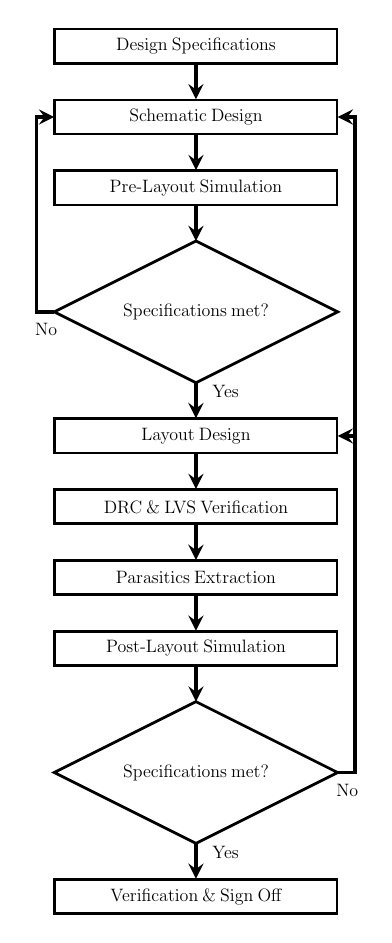
\begin{tikzpicture}[scale=0.45, transform shape]
        % Paths, nodes and wires:
        \node[shape=rectangle, draw, line width=1pt, minimum width=7.965cm, minimum height=0.965cm] at (5, 0.5){} node[anchor=center, align=center, text width=7.577cm, inner sep=6pt] at (5, 0.5){\Large Verification \& Sign Off};
        \draw[line width=1pt] (1, 17) -- (5, 19) -- (9, 17) -- (5, 15) -- (1, 17) -- cycle;
        \node[shape=rectangle, draw, line width=1pt, minimum width=7.965cm, minimum height=0.965cm] at (5, 20.5){} node[anchor=center, align=center, text width=7.577cm, inner sep=6pt] at (5, 20.5){\Large Pre-Layout Simulation};
        \node[shape=rectangle, draw, line width=1pt, minimum width=7.965cm, minimum height=0.965cm] at (5, 22.5){} node[anchor=center, align=center, text width=7.577cm, inner sep=6pt] at (5, 22.5){\Large Schematic Design};
        \node[shape=rectangle, draw, line width=1pt, minimum width=7.965cm, minimum height=0.965cm] at (5, 24.5){} node[anchor=center, align=center, text width=7.577cm, inner sep=6pt] at (5, 24.5){\Large Design Specifications};
        \draw[line width=1.4pt, -stealth] (5, 24) -| (5, 23);
        \draw[line width=1.4pt, -stealth] (5, 22) -| (5, 21);
        \draw[line width=1.4pt, -stealth] (5, 20) -| (5, 19);
        \node[shape=rectangle, minimum width=4.965cm, minimum height=0.715cm] at (5, 17){} node[anchor=center, align=center, text width=4.577cm, inner sep=6pt] at (5, 17){\Large Specifications met?};
        \node[shape=rectangle, draw, line width=1pt, minimum width=7.965cm, minimum height=0.965cm] at (5, 9.5){} node[anchor=center, align=center, text width=7.577cm, inner sep=6pt] at (5, 9.5){\Large Parasitics Extraction};
        \node[shape=rectangle, draw, line width=1pt, minimum width=7.965cm, minimum height=0.965cm] at (5, 11.5){} node[anchor=center, align=center, text width=7.577cm, inner sep=6pt] at (5, 11.5){\Large DRC \& LVS Verification};
        \node[shape=rectangle, draw, line width=1pt, minimum width=7.965cm, minimum height=0.965cm] at (5, 13.5){} node[anchor=center, align=center, text width=7.577cm, inner sep=6pt] at (5, 13.5){\Large Layout Design};
        \draw[line width=1.4pt, -stealth] (5, 13) -| (5, 12);
        \draw[line width=1.4pt, -stealth] (5, 11) -| (5, 10);
        \draw[line width=1.4pt, -stealth] (5, 9) -| (5, 8);
        \draw[line width=1pt] (1, 4) -- (5, 6) -- (9, 4) -- (5, 2) -- (1, 4) -- cycle;
        \node[shape=rectangle, minimum width=4.965cm, minimum height=0.715cm] at (5, 4){} node[anchor=center, align=center, text width=4.577cm, inner sep=6pt] at (5, 4){\Large Specifications met?};
        \draw[line width=1.4pt, -stealth] (5, 2) -| (5, 1);
        \draw[line width=1.4pt, -stealth] (1, 17) -| (0.5, 17.125) -- (0.5, 22.375) |- (1, 22.5);
        \node[shape=rectangle, draw, line width=1pt, minimum width=7.965cm, minimum height=0.965cm] at (5, 7.5){} node[anchor=center, align=center, text width=7.577cm, inner sep=6pt] at (5, 7.5){\Large Post-Layout Simulation};
        \draw[line width=1.4pt, -stealth] (5, 7) -| (5, 6);
        \draw[line width=1.4pt, -stealth] (5, 15) -| (5, 14);
        \node[shape=rectangle, minimum width=0.965cm, minimum height=0.465cm] at (0.75, 16.5){} node[anchor=center, align=center, text width=0.577cm, inner sep=6pt] at (0.75, 16.5){\Large No};
        \node[shape=rectangle, minimum width=0.965cm, minimum height=0.465cm] at (5.75, 14.75){} node[anchor=center, align=center, text width=0.577cm, inner sep=6pt] at (5.75, 14.75){\Large Yes};
        \node[shape=rectangle, minimum width=0.965cm, minimum height=0.465cm] at (9.25, 3.5){} node[anchor=center, align=center, text width=0.577cm, inner sep=6pt] at (9.25, 3.5){\Large No};
        \node[shape=rectangle, minimum width=0.965cm, minimum height=0.465cm] at (5.75, 1.75){} node[anchor=center, align=center, text width=0.577cm, inner sep=6pt] at (5.75, 1.75){\Large Yes};
        \draw[line width=1.4pt, -stealth] (9, 4) -- (9.5, 4) |- (9, 22.5);
        \draw[line width=1.4pt, -stealth] (9.5, 13.5) -- (9, 13.5);
    \end{tikzpicture}

    \caption{IC Design Flowchart} \label{fig:ic_design_flow}
\end{figure}

At this level, the schematics are simulated and validated against the target specifications, and the design is iteratively refined, adjusting topology and device sizing as needed, until the desired electrical performance is achieved at the schematic level.

Once the schematic-level design has been validated, the physical layout process begins. During this stage, device placement and interconnect routing are carried out, translating the schematic into the physical geometries that will define the fabrication masks, as discussed in Section~\ref{sec:layout_background}. Throughout this process, \ac{DRC} and \ac{LVS} verification are performed to ensure that the resulting layout complies with the geometric and electrical design rules specified by the foundry in the \ac{DRM}, and that the physical implementation is electrically equivalent to the validated schematic.

After the layout has successfully passed both \ac{DRC} and \ac{LVS} verification, the parasitic elements introduced by the physical implementation, such as parasitic resistances and capacitances associated with interconnect and device layout, are extracted from the physical design. A post-extraction validation of the design is then performed, in which the extracted parasitics are included in simulation, in order to characterize their impact on the overall system performance relative to the original schematic-level results.

If any of the target specifications are not met at this post-extraction stage, the design flow returns to the layout and, if necessary, the schematic stages, and the process is iteratively refined until the desired performance is achieved with the extracted parasitics included. This iterative schematic-layout-extraction loop, illustrated conceptually in Figure~\ref{fig:ic_design_flow}, is characteristic of high-speed analog and mixed-signal design, where layout parasitics can have a first-order impact on circuit performance. %and is followed throughout the design of the \ac{TX} driver presented in this dissertation.

\section{Layout} \label{sec:layout_background}

Layout design constitutes the final main step of the \ac{IC} design flow, carried out once the schematic-level design has been validated through pre-layout simulation and confirmed to meet the required functionality and performance specifications. During the layout stage, the schematic representation of the circuit is translated into a physical representation, defining the geometric shapes that will appear on the photomasks used during fabrication. The masks are created thorugh \ac{FEOL} processing, for the individual devices, and \ac{BEOL} processing, for the multi-layered interconnects~\cite{layout_fundamentals}.

This physical translation is not ideal, and inevitably introduces non-idealities, commonly referred to as parasitics, as well as layout-dependent effects that are difficult to predict accurately at the schematic level. These effects can alter the electrical characteristics and performance of the designed circuit relative to its pre-layout simulation results~\cite{layout_fundamentals, razavi}, making careful layout design essential for high-speed circuits, where performance margins are tight.

Layout-dependent effects can be broadly classified into two categories: manufacturing-related and environmental. Manufacturing-related effects include dopant concentration gradients, oxide thickness gradients, and mechanical stress, all of which are difficult to predict and simulate accurately, since they depend on the specific fabrication process and the physical layout of the design. Environmental effects primarily include temperature gradients across the die, which are similarly difficult to account for during the design phase, since they depend on the operating conditions and power dissipation profile of the final system~\cite{layout_fundamentals}.

Dopant gradients arise as a manufacturing imperfection resulting from non-uniformities in the ion implantation process, such as ion beam gradients and beam angle variations across the wafer. Temperature gradients, in contrast, are an environmental factor, encompassing both external temperature variations in the operating environment and self-heating effects caused by power dissipation within the circuit itself. Mechanical stress arises from both manufacturing and packaging imperfections, including material density variations across the die and thermal effects introduced during die-attach and wire-bonding processes.


\subsection{Device Sizing and Matching}\label{sec:device_matching} 

Device mismatch, that is, the deviation in electrical characteristics between devices that are nominally identical by design, can be classified into two main types: random mismatch and systematic mismatch. Systematic mismatches arises from layout-dependent effects and can, in principle, be predicted and compensated for through appropriate layout techniques, whereas random mismatches arises from inherently stochastic variations in the fabrication process~\cite{layout_fundamentals}.

\begin{figure}[h]
    \centering
    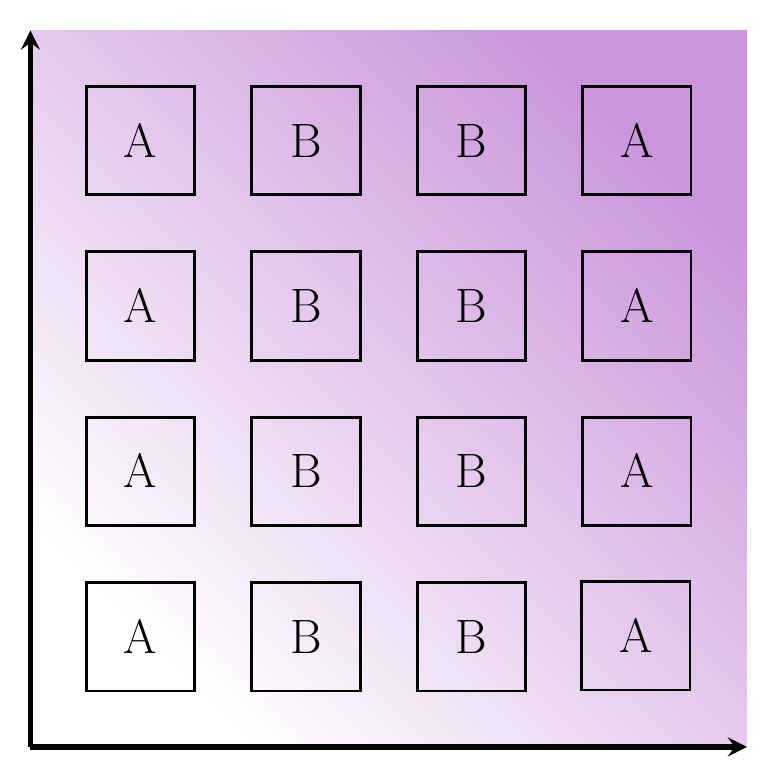
\begin{tikzpicture}[scale=0.7, transform shape]
        % Paths, nodes and wires:
        %\node[shape=rectangle, shade, right color={rgb,255:red,202;green,149;blue,219}, left color={rgb,255:red,255;green,255;blue,255}, draw={rgb,255:red,255;green,255;blue,255}, line width=1pt, minimum width=12.965cm, minimum height=12.965cm] at (6.5, 6.5){};
        \shade[left color={rgb,255:red,202;green,149;blue,219}, right color=white, shading angle=-45] (0,0) rectangle (13,13);
        \path[draw={rgb,255:red,0;green,0;blue,0}, line width=2pt, stealth-] (0, 13) -- (0, -0);
        \draw[line width=2pt, -stealth] (0, -0) -- (13, -0);
        \node[shape=rectangle, draw, line width=1pt, minimum width=1.965cm, minimum height=1.965cm] at (2, 11){} node[anchor=center, align=center, text width=1.577cm, inner sep=6pt] at (2, 11){\Huge A};
        \node[shape=rectangle, draw, line width=1pt, minimum width=1.965cm, minimum height=1.965cm] at (5, 11){} node[anchor=center, align=center, text width=1.577cm, inner sep=6pt] at (5, 11){\Huge B};
        \node[shape=rectangle, draw, line width=1pt, minimum width=1.965cm, minimum height=1.965cm] at (8, 11){} node[anchor=center, align=center, text width=1.577cm, inner sep=6pt] at (8, 11){\Huge B};
        \node[shape=rectangle, draw, line width=1pt, minimum width=1.965cm, minimum height=1.965cm] at (11, 11){} node[anchor=center, align=center, text width=1.577cm, inner sep=6pt] at (11, 11){\Huge A};
        \node[shape=rectangle, draw, line width=1pt, minimum width=1.965cm, minimum height=1.965cm] at (2, 8){} node[anchor=center, align=center, text width=1.577cm, inner sep=6pt] at (2, 8){\Huge A};
        \node[shape=rectangle, draw, line width=1pt, minimum width=1.965cm, minimum height=1.965cm] at (5, 8){} node[anchor=center, align=center, text width=1.577cm, inner sep=6pt] at (5, 8){\Huge B};
        \node[shape=rectangle, draw, line width=1pt, minimum width=1.965cm, minimum height=1.965cm] at (8, 8){} node[anchor=center, align=center, text width=1.577cm, inner sep=6pt] at (8, 8){\Huge B};
        \node[shape=rectangle, draw, line width=1pt, minimum width=1.965cm, minimum height=1.965cm] at (11, 8){} node[anchor=center, align=center, text width=1.577cm, inner sep=6pt] at (11, 8){\Huge A};
        \node[shape=rectangle, draw, line width=1pt, minimum width=1.965cm, minimum height=1.965cm] at (2, 5){} node[anchor=center, align=center, text width=1.577cm, inner sep=6pt] at (2, 5){\Huge A};
        \node[shape=rectangle, draw, line width=1pt, minimum width=1.965cm, minimum height=1.965cm] at (5, 5){} node[anchor=center, align=center, text width=1.577cm, inner sep=6pt] at (5, 5){\Huge B};
        \node[shape=rectangle, draw, line width=1pt, minimum width=1.965cm, minimum height=1.965cm] at (8, 5){} node[anchor=center, align=center, text width=1.577cm, inner sep=6pt] at (8, 5){\Huge B};
        \node[shape=rectangle, draw, line width=1pt, minimum width=1.965cm, minimum height=1.965cm] at (11, 5){} node[anchor=center, align=center, text width=1.577cm, inner sep=6pt] at (11, 5){\Huge A};
        \node[shape=rectangle, draw, line width=1pt, minimum width=1.965cm, minimum height=1.965cm] at (2, 2){} node[anchor=center, align=center, text width=1.577cm, inner sep=6pt] at (2, 2){\Huge A};
        \node[shape=rectangle, draw, line width=1pt, minimum width=1.965cm, minimum height=1.965cm] at (5, 2){} node[anchor=center, align=center, text width=1.577cm, inner sep=6pt] at (5, 2){\Huge B};
        \node[shape=rectangle, draw, line width=1pt, minimum width=1.965cm, minimum height=1.965cm] at (8, 2){} node[anchor=center, align=center, text width=1.577cm, inner sep=6pt] at (8, 2){\Huge B};
        \node[shape=rectangle, draw, line width=1pt, minimum width=1.965cm, minimum height=1.965cm] at (10.984, 2.016){} node[anchor=center, align=center, text width=1.577cm, inner sep=6pt] at (10.984, 2.016){\Huge A};
    \end{tikzpicture}
    \caption{Wafer gradient impact on devices}\label{fig:wafer_gradient}
\end{figure}

Systematic mismatch can be further divided into mask-related mismatch and gradient-related mismatch. Mask-related mismatch arises from mechanisms that affect all devices of a given size equally, and must therefore be accounted for at the schematic design stage rather than through layout techniques alone; a representative example is a systematic variation in the effective width or length of a device relative to its drawn dimensions. Gradient mismatch, in contrast, is caused by spatial process gradients across the die, and primarily affects devices that are physically separated from one another; matched devices should therefore be placed as close together as possible to minimize this effect. A representative example of gradient mismatch is the variation in threshold voltage caused by dopant concentration gradients across the die.
The influence of spatial process gradients on different device placements is illustrated in Figure~\ref{fig:wafer_gradient}.

Random mismatch arises from statistical fluctuations in processing conditions or material properties at the device level, and its magnitude is highly dependent on the physical dispersion, or spatial distribution, of the matched devices across the layout.

Each type of mismatch can be mitigated through specific layout strategies. Mask-related mismatch can be compensated by constructing each device as a parallel combination of multiple unit-sized devices, and by surrounding the active devices with dummy devices to ensure that all unit devices experience similar local surroundings during fabrication~\cite{layout_fundamentals, ndjountche2011_highspeed}. Gradient mismatch can be compensated by maximizing the size of the unit devices used, maximizing the area-to-perimeter ratio of each device (favoring square-like geometries), and placing matched devices as close together as possible. Random mismatch can be compensated by ensuring that matched devices share identical size, orientation, and, where possible, similar local placement, while also maximizing the spatial dispersion of the overall device distribution across the available layout area~\cite{layout_fundamentals,razavi,ndjountche2011_highspeed}.

More generally, distributing matched devices as evenly as possible across the layout helps reduce a wide range of unwanted effects, by ensuring that all devices are exposed to similar local conditions. Dummy devices are also essential in enabling an abuttable, modular layout design approach, since they allow standard-cell-like blocks to be placed directly adjacent to one another while preserving matching conditions at the block boundaries, which in turn helps reduce the overall area of the layout.

\subsubsection{Matching Techniques}\label{sec:matching_techniques}

\begin{figure}[H]
    \centering
    \begin{subfigure}{0.49\textwidth}
        \centering
        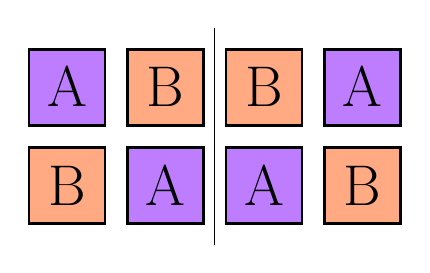
\begin{tikzpicture}[transform shape]
            % Paths, nodes and wires:
            \node[shape=rectangle, fill={rgb,255:red,190;green,125;blue,255}, draw, line width=1pt, minimum width=0.965cm, minimum height=0.965cm] at (0.5, 2){} node[anchor=center, align=center, text width=0.577cm, inner sep=6pt] at (0.5, 2){\huge A};
            \node[shape=rectangle, fill={rgb,255:red,255;green,170;blue,130}, draw, line width=1pt, minimum width=0.965cm, minimum height=0.965cm] at (0.5, 0.75){} node[anchor=center, align=center, text width=0.577cm, inner sep=6pt] at (0.5, 0.75){\huge B};
            \node[shape=rectangle, fill={rgb,255:red,255;green,170;blue,130}, draw, line width=1pt, minimum width=0.965cm, minimum height=0.965cm] at (1.75, 2){} node[anchor=center, align=center, text width=0.577cm, inner sep=6pt] at (1.75, 2){\huge B};
            \node[shape=rectangle, fill={rgb,255:red,190;green,125;blue,255}, draw, line width=1pt, minimum width=0.965cm, minimum height=0.965cm] at (1.75, 0.75){} node[anchor=center, align=center, text width=0.577cm, inner sep=6pt] at (1.75, 0.75){\huge A};
            \node[shape=rectangle, fill={rgb,255:red,190;green,125;blue,255}, draw, line width=1pt, minimum width=0.965cm, minimum height=0.965cm] at (3, 0.75){} node[anchor=center, align=center, text width=0.577cm, inner sep=6pt] at (3, 0.75){\huge A};
            \node[shape=rectangle, fill={rgb,255:red,255;green,170;blue,130}, draw, line width=1pt, minimum width=0.965cm, minimum height=0.965cm] at (3, 2){} node[anchor=center, align=center, text width=0.577cm, inner sep=6pt] at (3, 2){\huge B};
            \node[shape=rectangle, fill={rgb,255:red,255;green,170;blue,130}, draw, line width=1pt, minimum width=0.965cm, minimum height=0.965cm] at (4.25, 0.75){} node[anchor=center, align=center, text width=0.577cm, inner sep=6pt] at (4.25, 0.75){\huge B};
            \node[shape=rectangle, fill={rgb,255:red,190;green,125;blue,255}, draw, line width=1pt, minimum width=0.965cm, minimum height=0.965cm] at (4.25, 2){} node[anchor=center, align=center, text width=0.577cm, inner sep=6pt] at (4.25, 2){\huge A};
            \draw (2.375, 2.75) -- (2.375, -0);
        \end{tikzpicture}
        \caption{Interdigitation}
        \label{fig:interdigitation}
    \end{subfigure}
    \begin{subfigure}{0.49\textwidth}
        \centering
        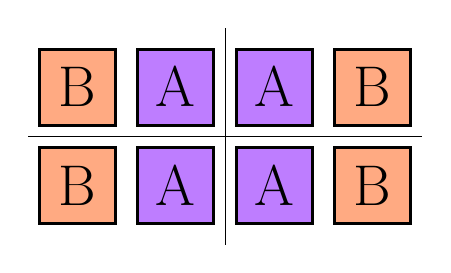
\begin{tikzpicture}[transform shape]
            % Paths, nodes and wires:
            \node[shape=rectangle, fill={rgb,255:red,190;green,125;blue,255}, draw, line width=1pt, minimum width=0.965cm, minimum height=0.965cm] at (2, 2){} node[anchor=center, align=center, text width=0.577cm, inner sep=6pt] at (2, 2){\huge A};
            \node[shape=rectangle, fill={rgb,255:red,255;green,170;blue,130}, draw, line width=1pt, minimum width=0.965cm, minimum height=0.965cm] at (0.75, 0.75){} node[anchor=center, align=center, text width=0.577cm, inner sep=6pt] at (0.75, 0.75){\huge B};
            \node[shape=rectangle, fill={rgb,255:red,255;green,170;blue,130}, draw, line width=1pt, minimum width=0.965cm, minimum height=0.965cm] at (0.75, 2){} node[anchor=center, align=center, text width=0.577cm, inner sep=6pt] at (0.75, 2){\huge B};
            \node[shape=rectangle, fill={rgb,255:red,190;green,125;blue,255}, draw, line width=1pt, minimum width=0.965cm, minimum height=0.965cm] at (2, 0.75){} node[anchor=center, align=center, text width=0.577cm, inner sep=6pt] at (2, 0.75){\huge A};
            \node[shape=rectangle, fill={rgb,255:red,190;green,125;blue,255}, draw, line width=1pt, minimum width=0.965cm, minimum height=0.965cm] at (3.25, 0.75){} node[anchor=center, align=center, text width=0.577cm, inner sep=6pt] at (3.25, 0.75){\huge A};
            \node[shape=rectangle, fill={rgb,255:red,255;green,170;blue,130}, draw, line width=1pt, minimum width=0.965cm, minimum height=0.965cm] at (4.5, 2){} node[anchor=center, align=center, text width=0.577cm, inner sep=6pt] at (4.5, 2){\huge B};
            \node[shape=rectangle, fill={rgb,255:red,255;green,170;blue,130}, draw, line width=1pt, minimum width=0.965cm, minimum height=0.965cm] at (4.5, 0.75){} node[anchor=center, align=center, text width=0.577cm, inner sep=6pt] at (4.5, 0.75){\huge B};
            \node[shape=rectangle, fill={rgb,255:red,190;green,125;blue,255}, draw, line width=1pt, minimum width=0.965cm, minimum height=0.965cm] at (3.25, 2){} node[anchor=center, align=center, text width=0.577cm, inner sep=6pt] at (3.25, 2){\huge A};
            \draw (2.625, 2.75) -- (2.625, -0);
            \draw (0.125, 1.375) -- (5.125, 1.375);
        \end{tikzpicture}
        \caption{Common centroid}
        \label{fig:common_centroid}
    \end{subfigure}
    \caption{Matching Patterns}\label{fig:matching_patterns}
\end{figure}

Both gradient and random mismatch can be further reduced through dedicated layout techniques that introduce symmetry into the device placement, such as interdigitation, common centroid, and the use of dummy devices~\cite{ndjountche2011_highspeed}. Interdigitation is a technique in which the matched devices are interleaved with one another along a single axis of symmetry. Common centroid is a technique in which the matched devices are arranged such that their geometric centroids coincide, using two orthogonal axes of symmetry; this arrangement creates symmetry in the layout and minimizes the impact of process gradients on the matched devices~\cite{razavi, layout_fundamentals}.
The interdigitated and common-centroid placement patterns are compared in Figure~\ref{fig:matching_patterns}.

\subsubsection{Well Proximity Effect}\label{sec:well_proximity_effect}

\begin{figure}[h]
    \centering
    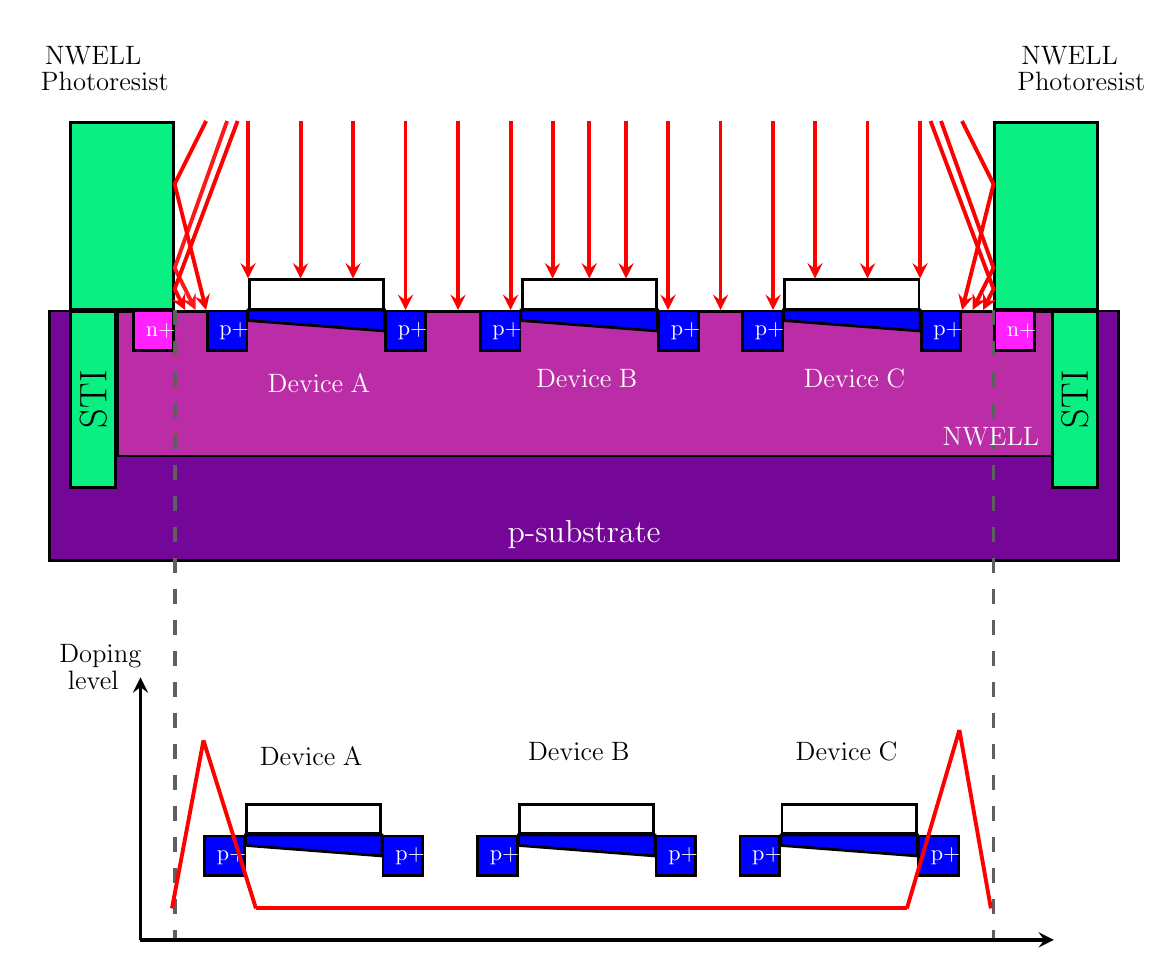
\begin{tikzpicture}[scale=0.8, transform shape]
        % Paths, nodes and wires:
        \node[shape=rectangle, fill={rgb,255:red,116;green,7;blue,152}, draw, line width=1pt, minimum width=16.965cm, minimum height=3.965cm] at (10.542, 10){} node[anchor=south, align=center, text width=16.577cm, inner sep=6pt] at (10.542, 8){\textcolor{rgb,255:red,255;green,255;blue,255}{\Large p-substrate}};
        \node[shape=rectangle, fill={rgb,255:red,187;green,45;blue,166}, draw, line width=1pt, minimum width=14.881cm, minimum height=2.298cm] at (10.583, 10.833){};
        \node[shape=rectangle, fill={rgb,255:red,10;green,239;blue,130}, draw, line width=1pt, minimum width=1.631cm, minimum height=2.965cm] at (3.208, 13.5){};
        \node[shape=rectangle, fill={rgb,255:red,10;green,239;blue,130}, draw, line width=1pt, minimum width=1.631cm, minimum height=2.965cm] at (17.875, 13.5){};
        \node[shape=rectangle, fill={rgb,255:red,10;green,239;blue,130}, draw, line width=1pt, minimum width=0.715cm, minimum height=2.798cm] at (18.333, 10.583){};
        \node[shape=rectangle, fill={rgb,255:red,10;green,239;blue,130}, draw, line width=1pt, minimum width=0.715cm, minimum height=2.798cm] at (2.75, 10.583){};
        \node[shape=rectangle, fill={rgb,255:red,255;green,34;blue,255}, draw, line width=1pt, minimum width=0.631cm, minimum height=0.631cm] at (3.708, 11.667){} node[anchor=center, align=center, text width=0.243cm, inner sep=6pt] at (3.708, 11.667){\textcolor{rgb,255:red,255;green,255;blue,255}{n+}};
        \node[shape=rectangle, fill={rgb,255:red,255;green,34;blue,255}, draw, line width=1pt, minimum width=0.631cm, minimum height=0.631cm] at (17.375, 11.667){} node[anchor=center, align=center, text width=0.243cm, inner sep=6pt] at (17.375, 11.667){\textcolor{rgb,255:red,255;green,255;blue,255}{n+}};
        \node[shape=rectangle, draw, line width=1pt, minimum width=2.131cm, minimum height=0.465cm] at (6.292, 12.25){};
        \draw[fill={rgb,255:red,0;green,0;blue,255}, line width=1pt] (5.208, 12) -- (5.208, 11.833) -- (7.375, 11.667) -- (7.375, 12) -- cycle;
        \node[shape=rectangle, fill={rgb,255:red,0;green,0;blue,255}, draw, line width=1pt, minimum width=0.631cm, minimum height=0.631cm] at (4.875, 11.667){} node[anchor=center, align=center, text width=0.243cm, inner sep=6pt] at (4.875, 11.667){\textcolor{rgb,255:red,255;green,255;blue,255}{p+}};
        \path[draw={rgb,255:red,251;green,26;blue,26}, line width=1.4pt, -stealth] (4.875, 15) -- (4.042, 12.667) -- (4.375, 12);
        \node[shape=rectangle, fill={rgb,255:red,0;green,0;blue,255}, draw, line width=1pt, minimum width=0.631cm, minimum height=0.631cm] at (7.708, 11.667){} node[anchor=center, align=center, text width=0.243cm, inner sep=6pt] at (7.708, 11.667){\textcolor{rgb,255:red,255;green,255;blue,255}{p+}};
        \path[draw={rgb,255:red,255;green,0;blue,0}, line width=1.4pt, stealth-] (4.208, 12) -- (4.042, 12.333) -- (5.042, 15);
        \path[draw={rgb,255:red,255;green,0;blue,0}, line width=1.4pt, -stealth] (4.542, 15) -- (4.042, 14) -- (4.542, 12);
        \node[shape=rectangle, draw, line width=1pt, minimum width=2.131cm, minimum height=0.465cm] at (14.792, 12.25){};
        \draw[fill={rgb,255:red,0;green,0;blue,255}, line width=1pt] (13.708, 12) -- (13.708, 11.833) -- (15.875, 11.667) -- (15.875, 12) -- cycle;
        \node[shape=rectangle, fill={rgb,255:red,0;green,0;blue,255}, draw, line width=1pt, minimum width=0.631cm, minimum height=0.631cm] at (13.375, 11.667){} node[anchor=center, align=center, text width=0.243cm, inner sep=6pt] at (13.375, 11.667){\textcolor{rgb,255:red,255;green,255;blue,255}{p+}};
        \node[shape=rectangle, fill={rgb,255:red,0;green,0;blue,255}, draw, line width=1pt, minimum width=0.631cm, minimum height=0.631cm] at (16.208, 11.667){} node[anchor=center, align=center, text width=0.243cm, inner sep=6pt] at (16.208, 11.667){\textcolor{rgb,255:red,255;green,255;blue,255}{p+}};
        \node[shape=rectangle, draw, line width=1pt, minimum width=2.131cm, minimum height=0.465cm] at (10.625, 12.25){};
        \draw[fill={rgb,255:red,0;green,0;blue,255}, line width=1pt] (9.542, 12) -- (9.542, 11.833) -- (11.708, 11.667) -- (11.708, 12) -- cycle;
        \node[shape=rectangle, fill={rgb,255:red,0;green,0;blue,255}, draw, line width=1pt, minimum width=0.631cm, minimum height=0.631cm] at (9.208, 11.667){} node[anchor=center, align=center, text width=0.243cm, inner sep=6pt] at (9.208, 11.667){\textcolor{rgb,255:red,255;green,255;blue,255}{p+}};
        \node[shape=rectangle, fill={rgb,255:red,0;green,0;blue,255}, draw, line width=1pt, minimum width=0.631cm, minimum height=0.631cm] at (12.042, 11.667){} node[anchor=center, align=center, text width=0.243cm, inner sep=6pt] at (12.042, 11.667){\textcolor{rgb,255:red,255;green,255;blue,255}{p+}};
        \path[draw={rgb,255:red,255;green,0;blue,0}, line width=1.4pt, stealth-] (16.875, 12) -- (17.042, 12.333) -- (16.042, 15);
        \path[draw={rgb,255:red,255;green,0;blue,0}, line width=1.4pt, stealth-] (16.708, 12) -- (17.042, 12.667) -- (16.208, 15);
        \path[draw={rgb,255:red,255;green,0;blue,0}, line width=1.4pt, stealth-] (16.542, 12) -- (17.042, 14) -- (16.542, 15);
        \path[draw={rgb,255:red,255;green,0;blue,0}, line width=1.4pt, -stealth] (5.208, 15) -- (5.208, 12.5);
        \path[draw={rgb,255:red,255;green,0;blue,0}, line width=1.4pt, -stealth] (6.042, 15) -- (6.042, 12.5);
        \path[draw={rgb,255:red,255;green,0;blue,0}, line width=1.4pt, -stealth] (6.875, 15) -- (6.875, 12.5);
        \path[draw={rgb,255:red,255;green,0;blue,0}, line width=1.4pt, -stealth] (7.708, 15) -- (7.708, 12);
        \path[draw={rgb,255:red,255;green,0;blue,0}, line width=1.4pt, -stealth] (8.542, 15) -- (8.542, 12);
        \path[draw={rgb,255:red,255;green,0;blue,0}, line width=1.4pt, -stealth] (9.375, 15) -- (9.375, 12);
        \path[draw={rgb,255:red,255;green,0;blue,0}, line width=1.4pt, -stealth] (14.208, 15) -- (14.208, 12.5);
        \path[draw={rgb,255:red,255;green,0;blue,0}, line width=1.4pt, -stealth] (15.042, 15) -- (15.042, 12.5);
        \path[draw={rgb,255:red,255;green,0;blue,0}, line width=1.4pt, -stealth] (15.875, 15) -- (15.875, 12.5);
        \path[draw={rgb,255:red,255;green,0;blue,0}, line width=1.4pt, -stealth] (11.875, 15) -- (11.875, 12);
        \path[draw={rgb,255:red,255;green,0;blue,0}, line width=1.4pt, -stealth] (12.708, 15) -- (12.708, 12);
        \path[draw={rgb,255:red,255;green,0;blue,0}, line width=1.4pt, -stealth] (13.542, 15) -- (13.542, 12);
        \path[draw={rgb,255:red,255;green,0;blue,0}, line width=1.4pt, -stealth] (10.042, 15) -- (10.042, 12.5);
        \path[draw={rgb,255:red,255;green,0;blue,0}, line width=1.4pt, -stealth] (11.208, 15) -- (11.208, 12.5);
        \path[draw={rgb,255:red,255;green,0;blue,0}, line width=1.4pt, -stealth] (10.625, 15) -- (10.625, 12.5);
        \node[shape=rectangle, rotate=90, minimum width=2.131cm, minimum height=0.965cm] at (18.333, 10.583){} node[anchor=center, align=center, text width=1.743cm, inner sep=6pt, rotate=90] at (18.333, 10.583){\LARGE STI};
        \node[shape=rectangle, rotate=90, minimum width=2.131cm, minimum height=0.965cm] at (2.75, 10.583){} node[anchor=center, align=center, text width=1.743cm, inner sep=6pt, rotate=90] at (2.75, 10.583){\LARGE STI};
        \node[shape=rectangle, minimum width=2.048cm, minimum height=1.298cm] at (2.75, 15.833){} node[anchor=center, align=center, text width=1.66cm, inner sep=6pt] at (2.75, 15.833){\large NWELL\\Photoresist};
        \node[shape=rectangle, minimum width=2.048cm, minimum height=1.298cm] at (18.25, 15.833){} node[anchor=center, align=center, text width=1.66cm, inner sep=6pt] at (18.25, 15.833){\large NWELL\\Photoresist};
        \node[shape=rectangle, minimum width=2.381cm, minimum height=0.798cm] at (6.333, 10.833){} node[anchor=center, align=center, text width=1.993cm, inner sep=6pt] at (6.333, 10.833){\textcolor{rgb,255:red,255;green,255;blue,255}{\large Device A}};
        \node[shape=rectangle, minimum width=2.381cm, minimum height=0.798cm] at (10.583, 10.917){} node[anchor=center, align=center, text width=1.993cm, inner sep=6pt] at (10.583, 10.917){\textcolor{rgb,255:red,255;green,255;blue,255}{\large Device B}};
        \node[shape=rectangle, minimum width=2.381cm, minimum height=0.798cm] at (14.833, 10.917){} node[anchor=center, align=center, text width=1.993cm, inner sep=6pt] at (14.833, 10.917){\textcolor{rgb,255:red,255;green,255;blue,255}{\large Device C}};
        \path[draw={rgb,255:red,95;green,95;blue,95}, line width=1.4pt, dash pattern={on 5.6pt off 5.6pt}] (4.042, 12) -- (4.042, 2);
        \path[draw={rgb,255:red,95;green,95;blue,95}, line width=1.4pt, dash pattern={on 5.6pt off 5.6pt}] (17.042, 12) -- (17.042, 2);
        \node[shape=rectangle, minimum width=2.381cm, minimum height=0.798cm] at (17, 10){} node[anchor=center, align=center, text width=1.993cm, inner sep=6pt] at (17, 10){\textcolor{rgb,255:red,255;green,255;blue,255}{\large NWELL}};
        \draw[line width=1.4pt, stealth-] (18, 2) -- (3.5, 2);
        \draw[line width=1.4pt, -stealth] (3.5, 2) -- (3.5, 6.167);
        \node[shape=rectangle, draw, line width=1pt, minimum width=2.131cm, minimum height=0.465cm] at (6.25, 3.917){};
        \draw[fill={rgb,255:red,0;green,0;blue,255}, line width=1pt] (5.167, 3.667) -- (5.167, 3.5) -- (7.333, 3.333) -- (7.333, 3.667) -- cycle;
        \node[shape=rectangle, fill={rgb,255:red,0;green,0;blue,255}, draw, line width=1pt, minimum width=0.631cm, minimum height=0.631cm] at (4.833, 3.333){} node[anchor=center, align=center, text width=0.243cm, inner sep=6pt] at (4.833, 3.333){\textcolor{rgb,255:red,255;green,255;blue,255}{p+}};
        \node[shape=rectangle, fill={rgb,255:red,0;green,0;blue,255}, draw, line width=1pt, minimum width=0.631cm, minimum height=0.631cm] at (7.667, 3.333){} node[anchor=center, align=center, text width=0.243cm, inner sep=6pt] at (7.667, 3.333){\textcolor{rgb,255:red,255;green,255;blue,255}{p+}};
        \node[shape=rectangle, draw, line width=1pt, minimum width=2.131cm, minimum height=0.465cm] at (14.75, 3.917){};
        \draw[fill={rgb,255:red,0;green,0;blue,255}, line width=1pt] (13.667, 3.667) -- (13.667, 3.5) -- (15.833, 3.333) -- (15.833, 3.667) -- cycle;
        \node[shape=rectangle, fill={rgb,255:red,0;green,0;blue,255}, draw, line width=1pt, minimum width=0.631cm, minimum height=0.631cm] at (13.333, 3.333){} node[anchor=center, align=center, text width=0.243cm, inner sep=6pt] at (13.333, 3.333){\textcolor{rgb,255:red,255;green,255;blue,255}{p+}};
        \node[shape=rectangle, fill={rgb,255:red,0;green,0;blue,255}, draw, line width=1pt, minimum width=0.631cm, minimum height=0.631cm] at (16.167, 3.333){} node[anchor=center, align=center, text width=0.243cm, inner sep=6pt] at (16.167, 3.333){\textcolor{rgb,255:red,255;green,255;blue,255}{p+}};
        \node[shape=rectangle, draw, line width=1pt, minimum width=2.131cm, minimum height=0.465cm] at (10.583, 3.917){};
        \draw[fill={rgb,255:red,0;green,0;blue,255}, line width=1pt] (9.5, 3.667) -- (9.5, 3.5) -- (11.667, 3.333) -- (11.667, 3.667) -- cycle;
        \node[shape=rectangle, fill={rgb,255:red,0;green,0;blue,255}, draw, line width=1pt, minimum width=0.631cm, minimum height=0.631cm] at (9.167, 3.333){} node[anchor=center, align=center, text width=0.243cm, inner sep=6pt] at (9.167, 3.333){\textcolor{rgb,255:red,255;green,255;blue,255}{p+}};
        \node[shape=rectangle, fill={rgb,255:red,0;green,0;blue,255}, draw, line width=1pt, minimum width=0.631cm, minimum height=0.631cm] at (12, 3.333){} node[anchor=center, align=center, text width=0.243cm, inner sep=6pt] at (12, 3.333){\textcolor{rgb,255:red,255;green,255;blue,255}{p+}};
        \node[shape=rectangle, minimum width=2.381cm, minimum height=0.798cm] at (6.208, 4.917){} node[anchor=center, align=center, text width=1.993cm, inner sep=6pt] at (6.208, 4.917){\large Device A};
        \node[shape=rectangle, minimum width=2.381cm, minimum height=0.798cm] at (10.458, 5){} node[anchor=center, align=center, text width=1.993cm, inner sep=6pt] at (10.458, 5){\large Device B};
        \node[shape=rectangle, minimum width=2.381cm, minimum height=0.798cm] at (14.708, 5){} node[anchor=center, align=center, text width=1.993cm, inner sep=6pt] at (14.708, 5){\large Device C};
        \path[draw={rgb,255:red,255;green,0;blue,0}, line width=1.4pt] (15.667, 2.5) -- (5.333, 2.5);
        \node[shape=rectangle, minimum width=1.465cm, minimum height=0.881cm] at (2.75, 6.333){} node[anchor=center, align=center, text width=1.077cm, inner sep=6pt] at (2.75, 6.333){\large Doping\\level};
        \path[draw={rgb,255:red,255;green,0;blue,0}, line width=1.4pt] (15.667, 2.5) -- (16.5, 5.333);
        \path[draw={rgb,255:red,255;green,0;blue,0}, line width=1.4pt] (16.5, 5.333) -- (17, 2.5);
        \path[draw={rgb,255:red,255;green,0;blue,0}, line width=1.4pt] (4, 2.5) -- (4.5, 5.167);
        \path[draw={rgb,255:red,255;green,0;blue,0}, line width=1.4pt] (4.5, 5.167) -- (5.333, 2.5);
    \end{tikzpicture}
    \caption{\ac{WPE} effect on the devices. Adapted from \cite{analoghub}}\label{fig:wpe_effect}
\end{figure}

An additional effect that must be considered during layout is the \ac{WPE}, which impacts the electrical characteristics of devices, such as threshold voltage, placed close to a well edge. This is caused by the lateral non-uniformity in the well doping process, during which, in the ion implantation process, high-energy ions reflect from the well photoresist and concentrate on the edges of the well, creating dopants gradient~\cite{razavi,layout_fundamentals}. This difference in dopant concentration causes mismatches between devices located near the wall edge. To counteract this effect, dummy devices can be placed around the matched core devices, providing sufficient separation between the core devices and the nearest well edge, and ensuring that all core devices experience equivalent local conditions, which helps minimize mask-related mismatch.
The device geometry associated with the well proximity effect is illustrated in Figure~\ref{fig:wpe_effect}.

\subsubsection{Length of Diffusion Effect}\label{sec:lod} %fig mostrando LOD e WPE

\ac{LOD} effect, also referred to as the \ac{STI} stress effect, is a manufacturing-induced effect in which mechanical stress is introduced at the edges of the active (diffusion) area during the formation of the \ac{STI} regions that isolate adjacent devices. This stress can cause variations in the threshold voltage of transistors located near the edges of their diffusion area, relative to devices with a larger surrounding active area, and is therefore an important consideration in the layout of matched analog devices~\cite{razavi,layout_fundamentals}.
The relationship between diffusion geometry and the \ac{LOD} effect is illustrated in Figure~\ref{fig:lod_effect}.

\begin{figure}[h]
    \centering
    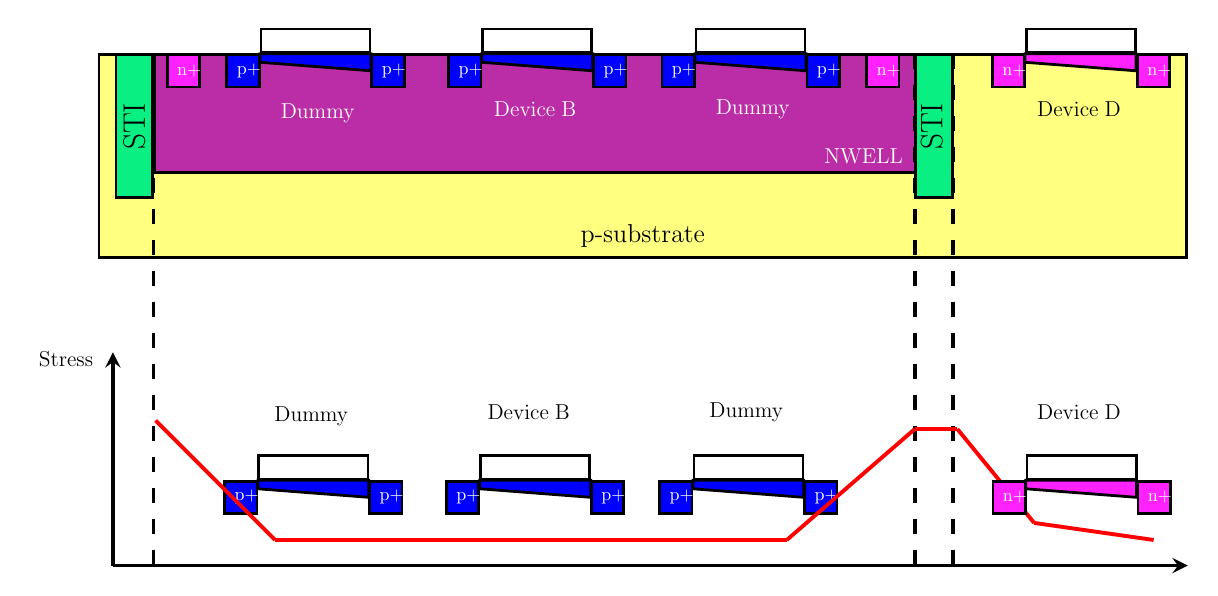
\begin{tikzpicture}[scale=0.65, transform shape]
        % Paths, nodes and wires:
        \node[shape=rectangle, fill={rgb,255:red,255;green,255;blue,128}, draw, line width=1pt, minimum width=21.256cm, minimum height=3.965cm] at (10.333, 8){} node[anchor=south, align=center, text width=20.868cm, inner sep=6pt] at (10.333, 6){\Large p-substrate};
        \node[shape=rectangle, fill={rgb,255:red,187;green,45;blue,166}, draw, line width=1pt, minimum width=14.881cm, minimum height=2.298cm] at (8.229, 8.833){};
        \node[shape=rectangle, fill={rgb,255:red,10;green,239;blue,130}, draw, line width=1pt, minimum width=0.715cm, minimum height=2.798cm] at (16.021, 8.583){};
        \node[shape=rectangle, fill={rgb,255:red,10;green,239;blue,130}, draw, line width=1pt, minimum width=0.715cm, minimum height=2.798cm] at (0.396, 8.583){};
        \node[shape=rectangle, fill={rgb,255:red,255;green,34;blue,255}, draw, line width=1pt, minimum width=0.631cm, minimum height=0.631cm] at (1.354, 9.667){} node[anchor=center, align=center, text width=0.243cm, inner sep=6pt] at (1.354, 9.667){\textcolor{rgb,255:red,255;green,255;blue,255}{n+}};
        \node[shape=rectangle, fill={rgb,255:red,255;green,34;blue,255}, draw, line width=1pt, minimum width=0.631cm, minimum height=0.631cm] at (15.021, 9.667){} node[anchor=center, align=center, text width=0.243cm, inner sep=6pt] at (15.021, 9.667){\textcolor{rgb,255:red,255;green,255;blue,255}{n+}};
        \node[shape=rectangle, draw, line width=1pt, minimum width=2.131cm, minimum height=0.465cm] at (3.937, 10.25){};
        \draw[fill={rgb,255:red,0;green,0;blue,255}, line width=1pt] (2.854, 10) -- (2.854, 9.833) -- (5.021, 9.667) -- (5.021, 10) -- cycle;
        \node[shape=rectangle, fill={rgb,255:red,0;green,0;blue,255}, draw, line width=1pt, minimum width=0.631cm, minimum height=0.631cm] at (2.521, 9.667){} node[anchor=center, align=center, text width=0.243cm, inner sep=6pt] at (2.521, 9.667){\textcolor{rgb,255:red,255;green,255;blue,255}{p+}};
        \node[shape=rectangle, fill={rgb,255:red,0;green,0;blue,255}, draw, line width=1pt, minimum width=0.631cm, minimum height=0.631cm] at (5.354, 9.667){} node[anchor=center, align=center, text width=0.243cm, inner sep=6pt] at (5.354, 9.667){\textcolor{rgb,255:red,255;green,255;blue,255}{p+}};
        \node[shape=rectangle, draw, line width=1pt, minimum width=2.131cm, minimum height=0.465cm] at (12.437, 10.25){};
        \draw[fill={rgb,255:red,0;green,0;blue,255}, line width=1pt] (11.354, 10) -- (11.354, 9.833) -- (13.521, 9.667) -- (13.521, 10) -- cycle;
        \node[shape=rectangle, fill={rgb,255:red,0;green,0;blue,255}, draw, line width=1pt, minimum width=0.631cm, minimum height=0.631cm] at (11.021, 9.667){} node[anchor=center, align=center, text width=0.243cm, inner sep=6pt] at (11.021, 9.667){\textcolor{rgb,255:red,255;green,255;blue,255}{p+}};
        \node[shape=rectangle, fill={rgb,255:red,0;green,0;blue,255}, draw, line width=1pt, minimum width=0.631cm, minimum height=0.631cm] at (13.854, 9.667){} node[anchor=center, align=center, text width=0.243cm, inner sep=6pt] at (13.854, 9.667){\textcolor{rgb,255:red,255;green,255;blue,255}{p+}};
        \node[shape=rectangle, draw, line width=1pt, minimum width=2.131cm, minimum height=0.465cm] at (8.271, 10.25){};
        \draw[fill={rgb,255:red,0;green,0;blue,255}, line width=1pt] (7.187, 10) -- (7.187, 9.833) -- (9.354, 9.667) -- (9.354, 10) -- cycle;
        \node[shape=rectangle, fill={rgb,255:red,0;green,0;blue,255}, draw, line width=1pt, minimum width=0.631cm, minimum height=0.631cm] at (6.854, 9.667){} node[anchor=center, align=center, text width=0.243cm, inner sep=6pt] at (6.854, 9.667){\textcolor{rgb,255:red,255;green,255;blue,255}{p+}};
        \node[shape=rectangle, fill={rgb,255:red,0;green,0;blue,255}, draw, line width=1pt, minimum width=0.631cm, minimum height=0.631cm] at (9.688, 9.667){} node[anchor=center, align=center, text width=0.243cm, inner sep=6pt] at (9.688, 9.667){\textcolor{rgb,255:red,255;green,255;blue,255}{p+}};
        \node[shape=rectangle, rotate=90, minimum width=2.131cm, minimum height=0.965cm] at (15.979, 8.583){} node[anchor=center, align=center, text width=1.743cm, inner sep=6pt, rotate=90] at (15.979, 8.583){\LARGE STI};
        \node[shape=rectangle, rotate=90, minimum width=2.131cm, minimum height=0.965cm] at (0.396, 8.583){} node[anchor=center, align=center, text width=1.743cm, inner sep=6pt, rotate=90] at (0.396, 8.583){\LARGE STI};
        \node[shape=rectangle, minimum width=2.381cm, minimum height=0.798cm] at (3.979, 8.833){} node[anchor=center, align=center, text width=1.993cm, inner sep=6pt] at (3.979, 8.833){\textcolor{rgb,255:red,255;green,255;blue,255}{\large Dummy}};
        \node[shape=rectangle, minimum width=2.381cm, minimum height=0.798cm] at (8.229, 8.917){} node[anchor=center, align=center, text width=1.993cm, inner sep=6pt] at (8.229, 8.917){\textcolor{rgb,255:red,255;green,255;blue,255}{\large Device B}};
        \node[shape=rectangle, minimum width=2.381cm, minimum height=0.798cm] at (12.479, 8.917){} node[anchor=center, align=center, text width=1.993cm, inner sep=6pt] at (12.479, 8.917){\textcolor{rgb,255:red,255;green,255;blue,255}{\large Dummy}};
        \path[draw={rgb,255:red,0;green,0;blue,0}, line width=1.4pt, dash pattern={on 5.6pt off 5.6pt}] (0.771, 10) -- (0.771, 0);
        \path[draw={rgb,255:red,0;green,0;blue,0}, line width=1.4pt, dash pattern={on 5.6pt off 5.6pt}] (15.646, 10) -- (15.646, -0);
        \node[shape=rectangle, minimum width=2.381cm, minimum height=0.798cm] at (14.646, 8){} node[anchor=center, align=center, text width=1.993cm, inner sep=6pt] at (14.646, 8){\textcolor{rgb,255:red,255;green,255;blue,255}{\large NWELL}};
        \draw[line width=1.4pt, stealth-] (20.979, -0) -- (-0.021, -0);
        \draw[line width=1.4pt, -stealth] (-0.021, -0) -- (-0.021, 4.167);
        \node[shape=rectangle, draw, line width=1pt, minimum width=2.131cm, minimum height=0.465cm] at (3.896, 1.917){};
        \draw[fill={rgb,255:red,0;green,0;blue,255}, line width=1pt] (2.813, 1.667) -- (2.813, 1.5) -- (4.979, 1.333) -- (4.979, 1.667) -- cycle;
        \node[shape=rectangle, fill={rgb,255:red,0;green,0;blue,255}, draw, line width=1pt, minimum width=0.631cm, minimum height=0.631cm] at (2.479, 1.333){} node[anchor=center, align=center, text width=0.243cm, inner sep=6pt] at (2.479, 1.333){\textcolor{rgb,255:red,255;green,255;blue,255}{p+}};
        \node[shape=rectangle, fill={rgb,255:red,0;green,0;blue,255}, draw, line width=1pt, minimum width=0.631cm, minimum height=0.631cm] at (5.313, 1.333){} node[anchor=center, align=center, text width=0.243cm, inner sep=6pt] at (5.313, 1.333){\textcolor{rgb,255:red,255;green,255;blue,255}{p+}};
        \node[shape=rectangle, draw, line width=1pt, minimum width=2.131cm, minimum height=0.465cm] at (12.396, 1.917){};
        \draw[fill={rgb,255:red,0;green,0;blue,255}, line width=1pt] (11.313, 1.667) -- (11.313, 1.5) -- (13.479, 1.333) -- (13.479, 1.667) -- cycle;
        \node[shape=rectangle, fill={rgb,255:red,0;green,0;blue,255}, draw, line width=1pt, minimum width=0.631cm, minimum height=0.631cm] at (10.979, 1.333){} node[anchor=center, align=center, text width=0.243cm, inner sep=6pt] at (10.979, 1.333){\textcolor{rgb,255:red,255;green,255;blue,255}{p+}};
        \node[shape=rectangle, fill={rgb,255:red,0;green,0;blue,255}, draw, line width=1pt, minimum width=0.631cm, minimum height=0.631cm] at (13.813, 1.333){} node[anchor=center, align=center, text width=0.243cm, inner sep=6pt] at (13.813, 1.333){\textcolor{rgb,255:red,255;green,255;blue,255}{p+}};
        \node[shape=rectangle, draw, line width=1pt, minimum width=2.131cm, minimum height=0.465cm] at (8.229, 1.917){};
        \draw[fill={rgb,255:red,0;green,0;blue,255}, line width=1pt] (7.146, 1.667) -- (7.146, 1.5) -- (9.313, 1.333) -- (9.313, 1.667) -- cycle;
        \node[shape=rectangle, fill={rgb,255:red,0;green,0;blue,255}, draw, line width=1pt, minimum width=0.631cm, minimum height=0.631cm] at (6.813, 1.333){} node[anchor=center, align=center, text width=0.243cm, inner sep=6pt] at (6.813, 1.333){\textcolor{rgb,255:red,255;green,255;blue,255}{p+}};
        \node[shape=rectangle, fill={rgb,255:red,0;green,0;blue,255}, draw, line width=1pt, minimum width=0.631cm, minimum height=0.631cm] at (9.646, 1.333){} node[anchor=center, align=center, text width=0.243cm, inner sep=6pt] at (9.646, 1.333){\textcolor{rgb,255:red,255;green,255;blue,255}{p+}};
        \node[shape=rectangle, minimum width=2.381cm, minimum height=0.798cm] at (3.854, 2.917){} node[anchor=center, align=center, text width=1.993cm, inner sep=6pt] at (3.854, 2.917){\large Dummy\\};
        \node[shape=rectangle, minimum width=2.381cm, minimum height=0.798cm] at (8.104, 3){} node[anchor=center, align=center, text width=1.993cm, inner sep=6pt] at (8.104, 3){\large Device B};
        \node[shape=rectangle, minimum width=2.381cm, minimum height=0.798cm] at (12.354, 3){} node[anchor=center, align=center, text width=1.993cm, inner sep=6pt] at (12.354, 3){\large Dummy};
        \path[draw={rgb,255:red,255;green,0;blue,0}, line width=1.4pt] (13.146, 0.5) -- (3.146, 0.5);
        \node[shape=rectangle, minimum width=1.465cm, minimum height=0.881cm] at (-0.937, 4.042){} node[anchor=center, align=center, text width=1.077cm, inner sep=6pt] at (-0.937, 4.042){\large Stress};
        \path[draw={rgb,255:red,255;green,0;blue,0}, line width=1.4pt] (13.146, 0.5) -- (15.646, 2.667);
        \path[draw={rgb,255:red,255;green,0;blue,0}, line width=1.4pt] (16.479, 2.667) -- (17.979, 0.833);
        \path[draw={rgb,255:red,255;green,0;blue,0}, line width=1.4pt] (0.813, 2.833) -- (3.146, 0.5);
        \node[shape=rectangle, draw, line width=1pt, minimum width=2.131cm, minimum height=0.465cm] at (18.896, 10.25){};
        \draw[fill={rgb,255:red,255;green,34;blue,255}, line width=1pt] (17.802, 10) -- (17.802, 9.833) -- (19.969, 9.667) -- (19.969, 10) -- cycle;
        \node[shape=rectangle, fill={rgb,255:red,255;green,34;blue,255}, draw, line width=1pt, minimum width=0.631cm, minimum height=0.631cm] at (17.479, 9.667){} node[anchor=center, align=center, text width=0.243cm, inner sep=6pt] at (17.479, 9.667){\textcolor{rgb,255:red,255;green,255;blue,255}{n+}};
        \node[shape=rectangle, fill={rgb,255:red,255;green,34;blue,255}, draw, line width=1pt, minimum width=0.631cm, minimum height=0.631cm] at (20.313, 9.667){} node[anchor=center, align=center, text width=0.243cm, inner sep=6pt] at (20.313, 9.667){\textcolor{rgb,255:red,255;green,255;blue,255}{n+}};
        \node[shape=rectangle, minimum width=2.381cm, minimum height=0.798cm] at (18.854, 8.917){} node[anchor=center, align=center, text width=1.993cm, inner sep=6pt] at (18.854, 8.917){\large Device D};
        \node[shape=rectangle, draw, line width=1pt, minimum width=2.131cm, minimum height=0.465cm] at (18.906, 1.917){};
        \draw[fill={rgb,255:red,255;green,34;blue,255}, line width=1pt] (17.813, 1.667) -- (17.813, 1.5) -- (19.979, 1.333) -- (19.979, 1.667) -- cycle;
        \node[shape=rectangle, fill={rgb,255:red,255;green,34;blue,255}, draw, line width=1pt, minimum width=0.631cm, minimum height=0.631cm] at (17.49, 1.333){} node[anchor=center, align=center, text width=0.243cm, inner sep=6pt] at (17.49, 1.333){\textcolor{rgb,255:red,255;green,255;blue,255}{n+}};
        \node[shape=rectangle, fill={rgb,255:red,255;green,34;blue,255}, draw, line width=1pt, minimum width=0.631cm, minimum height=0.631cm] at (20.323, 1.333){} node[anchor=center, align=center, text width=0.243cm, inner sep=6pt] at (20.323, 1.333){\textcolor{rgb,255:red,255;green,255;blue,255}{n+}};
        \path[draw={rgb,255:red,0;green,0;blue,0}, line width=1.4pt, dash pattern={on 5.6pt off 5.6pt}] (16.396, 10) -- (16.396, -0);
        \node[shape=rectangle, minimum width=2.381cm, minimum height=0.798cm] at (18.854, 3){} node[anchor=center, align=center, text width=1.993cm, inner sep=6pt] at (18.854, 3){\large Device D};
        \path[draw={rgb,255:red,255;green,0;blue,0}, line width=1.4pt] (15.646, 2.667) -- (16.479, 2.667);
        \path[draw={rgb,255:red,255;green,0;blue,0}, line width=1.4pt] (17.979, 0.833) -- (19.146, 0.667) -- (20.313, 0.5);
    \end{tikzpicture}
    \caption{\ac{LOD} effect on the devices. Adapted from \cite{analoghub}}\label{fig:lod_effect}
\end{figure}

The origin of the \ac{LOD} effect lies directly in the \ac{STI} formation process itself. As the wafer cools following \ac{STI} formation, the oxide-filled trenches become compressive, inducing mechanical stress on the adjacent silicon active area. The magnitude of this stress is strongly influenced by the width of the \ac{STI} region, that is, the spacing between neighboring active areas: devices with narrower active-to-active spacing experience a stronger stress effect than devices surrounded by wider isolation regions.

The compressive stress introduced by \ac{LOD} affects electron and hole mobility asymmetrically: it improves hole mobility while decreasing electron mobility, and therefore has an opposite effect on PMOS and NMOS device performance for a given active area geometry. Because this effect is strongly dependent on the distance between a device and the edge of its active area, \ac{LOD} can be mitigated by increasing the distance between the core devices and the surrounding well edge. In practice, this is achieved by surrounding the core devices with dummy devices~\cite{layout_fundamentals}, which increase the effective active area surrounding the matched devices and reduce the \ac{LOD}-induced variation between them.

\subsection{Routing and Signal Integrity}\label{sec:routing_si} %figs mostrando metal stack; interconnects proximos (paralelos e sobrepostos) e cap e res parasita; IR drop; EM; Antenna effect; diff signals e simetria

Routing interconnects must be carefully sized and spaced in order to minimize the parasitic effects they introduce, since these parasitics directly affect the signal integrity and reliability of the circuit. Parasitic capacitances and inductances appear between adjacent interconnects, altering signal propagation characteristics such as rise and fall times, and potentially introducing unwanted signal reflections and crosstalk between neighboring signal paths. In addition, interconnects introduce parasitic series resistance along the signal path, which causes unwanted voltage drops, commonly referred to as IR drop, that can affect signal timing, introduce additional RC delay~\cite{layout_fundamentals,bogatin_SI}, and reduce the effective switching speed of the devices being driven.

\subsubsection{IR Drop}\label{sec:ir_drop}

IR drop refers to the reduction in voltage available at a load node, caused by the voltage drop across the parasitic resistance of the interconnect supplying it. The magnitude of the IR drop is directly proportional to the current flowing through the interconnect and to its parasitic resistance, and, if left unmitigated, can lead to timing violations and signal integrity degradation~\cite{layout_fundamentals}. IR drop can be reduced by increasing the width of the interconnect, thereby lowering its resistance, or by using lower-resistance routing materials where available.

IR drop is particularly critical in power delivery networks, where the combination of high current densities and long interconnect lengths can result in significant voltage drops across the network, degrading both the performance and long-term reliability of the entire system~\cite{dally_poulton_1998}. To mitigate IR drop in the power delivery network routing, designers can employ wider interconnects, use lower-resistance metal layers, and carefully place vias to minimize the resistive path between the supply source and the load devices.

\subsubsection{Parasitic Capacitances}\label{sec:parasitic_cap}

To minimize parasitic capacitance, interconnects should be routed as short as possible and placed as far as practical from neighboring interconnects. Where interconnects on different metal layers are routed in close proximity or overlap vertically, the voltage differential and signal activity present on the overlapping layers should be carefully considered and analyzed, since capacitive coupling between them can introduce unwanted crosstalk or timing-dependent noise~\cite{layout_fundamentals,bogatin_SI}.
The coupling geometry between nearby metal interconnects is illustrated in Figure~\ref{fig:parasitic_capacitances}, in both top and cross-sectional views.

\begin{figure}[h]
    \centering
    \begin{subfigure}{0.49\textwidth}
        \centering
        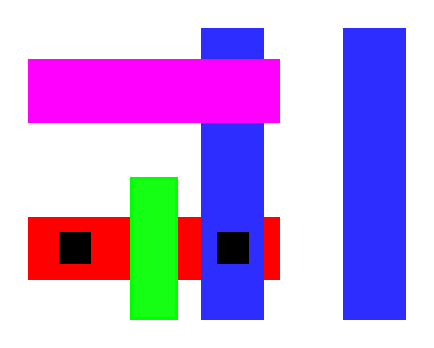
\begin{tikzpicture}[scale=0.8, transform shape]
            % Paths, nodes and wires:
            \node[shape=rectangle, fill={rgb,255:red,255;green,0;blue,0}, draw={rgb,255:red,255;green,0;blue,0}, line width=1pt, minimum width=3.965cm, minimum height=0.965cm] at (2, 1.125){};
            \node[shape=rectangle, fill={rgb,255:red,0;green,0;blue,0}, draw, line width=1pt, minimum width=0.465cm, minimum height=0.465cm] at (0.75, 1.125){};
            \node[shape=rectangle, fill={rgb,255:red,45;green,45;blue,255}, draw={rgb,255:red,45;green,45;blue,255}, line width=1pt, minimum width=0.965cm, minimum height=4.59cm] at (3.25, 2.313){};
            \node[shape=rectangle, fill={rgb,255:red,0;green,0;blue,0}, draw, line width=1pt, minimum width=0.465cm, minimum height=0.465cm] at (3.25, 1.125){};
            \node[shape=rectangle, fill={rgb,255:red,21;green,255;blue,21}, draw={rgb,255:red,0;green,255;blue,0}, line width=1pt, minimum width=0.715cm, minimum height=2.215cm] at (2, 1.125){};
            \node[shape=rectangle, fill={rgb,255:red,255;green,0;blue,255}, draw={rgb,255:red,255;green,0;blue,255}, line width=1pt, minimum width=3.965cm, minimum height=0.965cm] at (2, 3.625){};
            \node[shape=rectangle, fill={rgb,255:red,45;green,45;blue,255}, draw={rgb,255:red,45;green,45;blue,255}, line width=1pt, minimum width=0.965cm, minimum height=4.59cm] at (5.5, 2.313){};
        \end{tikzpicture}
        \caption{Top view}
    
    \end{subfigure}
    \begin{subfigure}{0.49\textwidth}
        \centering
        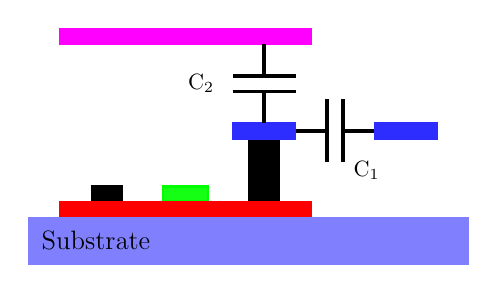
\begin{tikzpicture}[scale=0.8, transform shape]
            % Paths, nodes and wires:
            \node[shape=rectangle, fill={rgb,255:red,21;green,255;blue,21}, draw={rgb,255:red,0;green,255;blue,0}, line width=1pt, minimum width=0.715cm, minimum height=0.215cm] at (2.5, 1.125){};
            \node[shape=rectangle, fill={rgb,255:red,0;green,0;blue,0}, draw, line width=1pt, minimum width=0.465cm, minimum height=1.215cm] at (3.75, 1.625){};
            \node[shape=rectangle, fill={rgb,255:red,0;green,0;blue,0}, draw, line width=1pt, minimum width=0.465cm, minimum height=0.215cm] at (1.25, 1.125){};
            \node[shape=rectangle, fill={rgb,255:red,45;green,45;blue,255}, draw={rgb,255:red,45;green,45;blue,255}, line width=1pt, minimum width=0.965cm, minimum height=0.215cm] at (3.75, 2.125){};
            \node[shape=rectangle, fill={rgb,255:red,45;green,45;blue,255}, draw={rgb,255:red,45;green,45;blue,255}, line width=1pt, minimum width=0.965cm, minimum height=0.215cm] at (6, 2.125){};
            \node[shape=rectangle, fill={rgb,255:red,255;green,0;blue,255}, draw={rgb,255:red,255;green,0;blue,255}, line width=1pt, minimum width=3.965cm, minimum height=0.215cm] at (2.5, 3.625){};
            \node[shape=rectangle, fill={rgb,255:red,255;green,0;blue,0}, draw={rgb,255:red,255;green,0;blue,0}, line width=1pt, minimum width=3.965cm, minimum height=0.215cm] at (2.5, 0.875){};
            \draw[line width=1.4pt] (4.25, 2.125) -- (4.75, 2.125);
            \draw[line width=1.4pt] (4.75, 2.625) -- (4.75, 1.625);
            \draw[line width=1.4pt] (5, 2.625) -- (5, 1.625);
            \draw[line width=1.4pt] (5, 2.125) -- (5.5, 2.125);
            \draw[line width=1.4pt] (3.25, 3) -- (4.25, 3);
            \draw[line width=1.4pt] (3.25, 2.75) -- (4.25, 2.75);
            \draw[line width=1.4pt] (3.75, 3) -- (3.75, 3.5);
            \draw[line width=1.4pt] (3.75, 2.25) -- (3.75, 2.75);
            \node[shape=rectangle, fill={rgb,255:red,128;green,128;blue,255}, draw={rgb,255:red,128;green,128;blue,255}, line width=1pt, minimum width=6.965cm, minimum height=0.715cm] at (3.5, 0.375){} node[anchor=north west, align=left, text width=6.577cm, inner sep=6pt] at (0, 0.75){\large Substrate};
            \node[shape=rectangle, minimum width=0.715cm, minimum height=0.715cm] at (5.375, 1.5){} node[anchor=center, align=center, text width=0.5cm, inner sep=6pt] at (5.375, 1.5){$\mathrm{C_1}$};
            \node[shape=rectangle, minimum width=0.715cm, minimum height=0.715cm] at (2.75, 2.875){} node[anchor=center, align=center, text width=0.5cm, inner sep=6pt] at (2.75, 2.875){$\mathrm{C_2}$};
        \end{tikzpicture}
        \caption{Cross section}
    \end{subfigure}

    \caption{Parasitic capacitances between different metal layers}\label{fig:parasitic_capacitances}
\end{figure}

Another consideration to be taken into account is the introduction of a parasitic Miller capacitance on devices with metal tracks connected to their drain and source terminals in close proximity. This parasitic capacitance results in the Miller effect, which makes the input capacitance of the device appear much larger than its actual value, and leads to a decrease in the switching speed of the device, limiting its bandwidth and causing unwanted delays, reducing overall performance.

%\subsubsection{Crosstalk}\label{sec:crosstalk}

%The choice of metal layer, as well as the width of each interconnect, must also be selected based on the current density expected to flow through it, in order to avoid \ac{EM}, a reliability concern that can lead to interconnect failure over time~\cite{EM_inside_logic_cells}. \ac{EM} is a phenomenon in which momentum transfer from conducting electrons to the metal lattice atoms causes gradual migration of the metal atoms themselves, eventually leading to void formation within the interconnect and, ultimately, to interconnect failure. The risk of \ac{EM} increases with higher current densities and elevated operating temperatures~\cite{black_EM,rzepka_self_heating_1998}, making it essential to design interconnects with sufficient width and appropriate metal layer selection to keep current density within the safe limits specified by the \ac{DRM}.

\subsubsection{Electromigration}\label{sec:electromigration}
The dimensions of an \ac{IC} interconnect cannot be determined solely from its parasitic resistance and capacitance. The amount of current carried by the metal must also be considered in order to ensure long-term reliability. One of the main current-related reliability mechanisms in metallic interconnects is \ac{EM}, which results from the transfer of momentum from conducting electrons to the metal atoms. Over time, this process produces a net transport of material along the interconnect, potentially creating regions of material depletion and accumulation. Material depletion can eventually form voids that increase the local resistance and may ultimately produce an open circuit~\cite{layout_fundamentals,EM_inside_logic_cells,black_EM}.
The severity of \ac{EM} is strongly related to the current density in the interconnect. For a metal line with width $w_m$ and thickness $t_m$, the cross-sectional area available for current conduction is

\begin{equation}
A_m = w_m t_m ,
\label{eq:metal_cross_section}
\end{equation}
and the instantaneous current density is therefore defined as~\cite{layout_fundamentals}
\begin{equation}
J(t) = \frac{i(t)}{A_m} = \frac{i(t)}{w_m t_m}
\label{eq:em_current_density}
\end{equation}

where $i(t)$ is the current flowing through the interconnect. The physical current density $J$ is expressed in $\mathrm{A/m^2}$, although $\mathrm{A/cm^2}$ or $\mathrm{MA/cm^2}$ are also commonly used for \ac{IC} interconnects.
Since the thickness of a given metal layer is fixed by the fabrication process, current-carrying capability is also commonly expressed as a current per unit width. Defining this width-normalized quantity as $J_w$ gives

\begin{equation}
J_w(t) = \frac{i(t)}{w_m} = J(t)t_m
\label{eq:em_current_per_width}
\end{equation}

Consequently, for a given metal layer and current, increasing the routing width directly reduces the current density. This relationship explains why electromigration constraints often impose a minimum interconnect width for nets carrying large currents. Higher metal layers may also provide greater current-carrying capability because they are generally thicker and therefore present a larger cross-sectional area~\cite{razavi,layout_fundamentals}.
For time-varying currents, a single instantaneous value is insufficient to characterize the electrical and thermal stress applied to the interconnect. Three current quantities are commonly considered: the peak, average, and \ac{RMS} currents. For a periodic, unidirectional current waveform $i(t)$ with period $T$, these quantities can be written as

\begin{align}
    I_{\mathrm{peak}} &= \max_{0\leq t<T}{i(t)}
    \label{eq:em_ipeak} \\
    I_{\mathrm{avg}} &= \frac{1}{T} \int_{0}^{T} i(t)dt
    \label{eq:em_iavg} \\
    I_{\mathrm{RMS}} &= \sqrt{\frac{1}{T} \int_{0}^{T} i^2(t)dt}
    \label{eq:em_irms}
\end{align}

The corresponding current densities follow directly from the interconnect cross-sectional area:

\begin{align}
    J_{\mathrm{peak}} &= \frac{I_{\mathrm{peak}}}{w_m t_m}
    \label{eq:em_jpeak} \\
    J_{\mathrm{avg}} &= \frac{I_{\mathrm{avg}}}{w_m t_m}
    \label{eq:em_javg}
    \\
    J_{\mathrm{RMS}} &= \frac{I_{\mathrm{RMS}}}{w_m t_m}
    \label{eq:em_jrms}
\end{align}
These quantities represent different forms of stress on the interconnect. The average current density is associated with the long-term net transport of metal caused by \ac{EM}, whereas the RMS current density is particularly relevant to Joule self-heating because the dissipated power is proportional to the square of the current~\cite{rzepka_self_heating_1998}. The peak current desnity characterizes the maximum instantaneous electrical stress and can become particularly relevant for short-duration or high-frequency current pulses. For this reason, technology design rules may specify different \ac{EM} limits for average, \ac{RMS}, and peak current depending on the type and duration of the waveform.
The relationship between these quantities can be illustrated by considering a periodic rectangular current pulse of amplitude $I_{\mathrm{peak}}$, active for a time $t_{\mathrm{on}}$ during each period $T$. Defining the duty cycle as

\begin{equation}
    D = \frac{t_{\mathrm{on}}}{T}
    \label{eq:em_duty_cycle}
    \end{equation}
    the average and RMS currents become
    \begin{align}
    I_{\mathrm{avg}} &= D I_{\mathrm{peak}}
    \label{eq:em_pulse_iavg}
    \\
    I_{\mathrm{RMS}} &= \sqrt{D}I_{\mathrm{peak}}
    \label{eq:em_pulse_irms}
\end{align}

Since the interconnect geometry is unchanged, the same relationships apply directly to current density:

\begin{align}
    J_{\mathrm{avg}} &= D J_{\mathrm{peak}}
    \label{eq:em_pulse_javg}
    \\
    J_{\mathrm{RMS}} &= \sqrt{D}J_{\mathrm{peak}}
    \label{eq:em_pulse_jrms}
\end{align}

Equivalently, if the average current density is kept constant while the duty cycle is reduced,

\begin{align}
    J_{\mathrm{peak}} &= \frac{J_{\mathrm{avg}}}{D}
    \label{eq:em_peak_from_avg}
    \\
    J_{\mathrm{RMS}} &= \frac{J_{\mathrm{avg}}}{\sqrt{D}}
    \label{eq:em_rms_from_avg}
\end{align}


This distinction is particularly important for high-speed digital interconnects. \cite{rzepka_self_heating_1998} show that two current waveforms having the same average current density can exhibit substantially different \ac{RMS} and peak current densities as their duty cycles change~\cite{rzepka_self_heating_1998}. Since the temperature rise caused by Joule heating increases approximately with the square of the current density, a low-duty-cycle waveform can satisfy an average-current constraint while still producing significant thermal stress. The resulting temperature increase is itself detrimental to electromigration lifetime, making current density and operating temperature coupled reliability considerations.
Current density can additionally be reduced by distributing the total current among multiple parallel interconnect paths. If a total current $I_{\mathrm{tot}}$ is divided approximately equally among $N$ identical metal tracks, the current carried by each track is

\begin{equation}
    I_{\mathrm{path}} \approx \frac{I_{\mathrm{tot}}}{N}
    \label{eq:em_parallel_current}
\end{equation}

and the corresponding current density becomes

\begin{equation}
J_{\mathrm{path}} \approx \frac{I_{\mathrm{tot}}}{N w_m t_m}
\label{eq:em_parallel_density}
\end{equation}

Therefore, increasing the metal width, selecting a thicker metal layer, or dividing the current among several parallel paths reduces the current density experienced by each individual interconnect. These principles are fundamental when routing high-current nets, and the routing interconnects should be designed according to the \ac{EM} limits defined by the technology \ac{DRM}.

%\subsubsection{Antenna Effect}\label{sec:antenna_effect}

%The antenna effect, also referred to as \ac{PID}, is a fabrication-related reliability concern that occurs when charge accumulates on electrically isolated nodes of the integrated circuit during processing, particularly during plasma etching steps. The energetic ions and radicals present in the plasma can accumulate on exposed interconnects, raising their electrical potential~\cite{layout_fundamentals, art_of_analog_layout,razavi}. If such an interconnect is connected to the gate of a transistor, the accumulated charge may discharge through the thin gate oxide, potentially causing permanent damage or gradual degradation of the device. The severity of this risk depends on the surface area of the interconnect exposed during the affected fabrication step: larger interconnect areas can accumulate higher potentials, increasing the likelihood of gate oxide breakdown and permanent device damage.

%Several layout techniques can be used to mitigate antenna violations. One common technique, referred to as metal jumping, consists of rerouting long interconnects to higher metal layers, typically near the load, since higher metal layers are deposited later in the fabrication process and are therefore not exposed to the earlier plasma processing steps that cause charge accumulation~\cite{layout_fundamentals, razavi}; this technique, however, may increase overall routing congestion. A second technique consists of reducing via area, since large via cut areas can themselves contribute to antenna violations; converting multi-cut vias to double-cut or single-cut vias reduces the exposed cut area, although this may introduce reliability concerns of its own, such as an increased susceptibility to electromigration. A third technique consists of inserting a diode near the affected gate, connected on a lower metal layer, to provide a controlled path for dissipating accumulated charge~\cite{art_of_analog_layout}; the diode is connected in reverse bias, with its cathode tied to the gate node and its anode tied to ground, providing a safe discharge path for static charge that would otherwise accumulate on the gate.

\subsubsection{Differential Signaling and Routing Symmetry}\label{sec:differential_routing_symmetry}

For systems employing differential signaling, such as the \ac{TX} driver discussed in this dissertation, the layout floorplan must be carefully designed to ensure symmetry between the two complementary signal paths, so that both paths experience equivalent parasitic effects and the differential characteristics of the signal are preserved\cite{chen_cml_review_2026}. This consideration is particularly important for high-speed signals, where differences in parasitic capacitance, resistance, or coupling between the two paths can lead to significant signal degradation, duty-cycle distortion, and timing mismatches between the differential signal pair~\cite{layout_fundamentals,bogatin_SI}.

\begin{figure}[H]
    \centering
    \begin{tikzpicture}[scale=0.8, transform shape]
        % Paths, nodes and wires:
        \node[shape=rectangle, fill={rgb,255:red,255;green,0;blue,0}, draw={rgb,255:red,255;green,0;blue,0}, line width=1pt, minimum width=3.965cm, minimum height=0.965cm] at (4.375, 1){};
        \node[shape=rectangle, fill={rgb,255:red,45;green,45;blue,255}, draw={rgb,255:red,45;green,45;blue,255}, line width=1pt, minimum width=0.965cm, minimum height=4.715cm] at (5.625, 2.375){};
        \node[shape=rectangle, fill={rgb,255:red,21;green,255;blue,21}, draw={rgb,255:red,0;green,255;blue,0}, line width=1pt, minimum width=0.715cm, minimum height=1.715cm] at (4.375, 1.125){};
        \node[shape=rectangle, fill={rgb,255:red,0;green,0;blue,0}, draw, line width=1pt, minimum width=0.465cm, minimum height=0.465cm] at (5.625, 1){};
        \node[shape=rectangle, fill={rgb,255:red,0;green,0;blue,0}, draw, line width=1pt, minimum width=0.465cm, minimum height=0.465cm] at (3.125, 1){};
        \node[shape=rectangle, fill={rgb,255:red,255;green,0;blue,255}, draw={rgb,255:red,255;green,0;blue,255}, line width=1pt, minimum width=4.965cm, minimum height=0.965cm] at (3.875, 4){};
        \node[shape=rectangle, fill={rgb,255:red,0;green,221;blue,221}, draw={rgb,255:red,0;green,221;blue,221}, line width=1pt, minimum width=1.715cm, minimum height=4.215cm] at (2.375, 5.375){};
        \node[shape=rectangle, fill={rgb,255:red,0;green,0;blue,0}, draw, line width=1pt, minimum width=0.465cm, minimum height=0.465cm] at (5.625, 4){};
        \node[shape=rectangle, fill={rgb,255:red,0;green,0;blue,0}, draw, line width=1pt, minimum width=0.465cm, minimum height=0.465cm] at (2.375, 4){};
        \node[shape=rectangle, fill={rgb,255:red,255;green,0;blue,0}, draw={rgb,255:red,255;green,0;blue,0}, line width=1pt, minimum width=3.965cm, minimum height=0.965cm] at (-0.625, 1){};
        \node[shape=rectangle, fill={rgb,255:red,45;green,45;blue,255}, draw={rgb,255:red,45;green,45;blue,255}, line width=1pt, minimum width=0.965cm, minimum height=4.715cm] at (-1.875, 2.375){};
        \node[shape=rectangle, fill={rgb,255:red,21;green,255;blue,21}, draw={rgb,255:red,0;green,255;blue,0}, line width=1pt, minimum width=0.715cm, minimum height=1.715cm] at (-0.625, 1.125){};
        \node[shape=rectangle, fill={rgb,255:red,0;green,0;blue,0}, draw, line width=1pt, minimum width=0.465cm, minimum height=0.465cm] at (0.625, 1){};
        \node[shape=rectangle, fill={rgb,255:red,0;green,0;blue,0}, draw, line width=1pt, minimum width=0.465cm, minimum height=0.465cm] at (-1.875, 1){};
        \node[shape=rectangle, fill={rgb,255:red,255;green,0;blue,255}, draw={rgb,255:red,255;green,0;blue,255}, line width=1pt, minimum width=3.965cm, minimum height=0.715cm] at (-3.125, 4.125){};
        \node[shape=rectangle, fill={rgb,255:red,0;green,0;blue,0}, draw, line width=1pt, minimum width=0.465cm, minimum height=0.465cm] at (-1.875, 4.125){};
        \node[shape=rectangle, fill={rgb,255:red,0;green,221;blue,221}, draw={rgb,255:red,0;green,221;blue,221}, line width=1pt, minimum width=0.965cm, minimum height=3.965cm] at (-4.375, 5.5){};
        \node[shape=rectangle, fill={rgb,255:red,0;green,0;blue,0}, draw, line width=1pt, minimum width=0.465cm, minimum height=0.465cm] at (-4.375, 4.125){};
        \node[shape=rectangle, fill={rgb,255:red,0;green,221;blue,221}, draw={rgb,255:red,0;green,221;blue,221}, line width=1pt, minimum width=0.965cm, minimum height=6.965cm] at (-6.625, 4){};
        \draw (-1.875, 3.25) to[american resistor, l={$\mathrm{R_1}$}, label distance=0.22cm] (-1.875, 1.75);
        \draw (5.625, 3.125) to[american resistor, l={$\mathrm{R_1}$}, label distance=0.22cm] (5.625, 1.625);
        \draw (-3.625, 4.125) to[american resistor, l={$\mathrm{R'_2}$}] (-2.375, 4.125);
        \draw (3.625, 4) to[american resistor, l={$\mathrm{R_2}$}, label distance=-0.04cm] (4.875, 4);
        \draw (2.375, 7.25) to[american resistor, l={$\mathrm{R_3}$}] (2.375, 5.5);
        \draw (-4.375, 7.25) to[american resistor, l={$\mathrm{R'_3}$}] (-4.375, 5.5);
        \draw[line width=1pt] (-5.625, 5.75) -- (-5.625, 4.75);
        \draw[line width=1pt] (-5.375, 5.75) -- (-5.375, 4.75);
        \draw[line width=1pt] (-5.625, 5.25) -- (-6.625, 5.25);
        \draw[line width=1pt] (-5.375, 5.25) -| (-4.375, 5.25);
        \draw[line width=1pt, stealth-stealth] (1.5, 7.75) -- (3.25, 7.75);
        \draw[line width=1pt] (3.25, 8) -| (3.25, 7.5);
        \draw[line width=1pt] (1.5, 8) -| (1.5, 7.5);
        \draw[line width=1pt, stealth-stealth] (6.625, 4.5) -| (6.625, 3.5);
        \draw[line width=1pt] (6.375, 4.5) -| (6.875, 4.5);
        \draw[line width=1pt] (6.375, 3.5) -| (6.875, 3.5);
        \draw[line width=1pt, stealth-stealth] (5.125, 5) -- (6.125, 5);
        \draw[line width=1pt] (6.125, 5.25) -| (6.125, 4.75);
        \draw[line width=1pt] (5.125, 5.25) -| (5.125, 4.75);
        \draw[line width=1pt, stealth-stealth] (-4.875, 7.75) -- (-3.875, 7.75);
        \draw[line width=1pt] (-3.875, 8) -| (-3.875, 7.5);
        \draw[line width=1pt] (-4.875, 8) -| (-4.875, 7.5);
        \draw[line width=1pt, stealth-stealth] (-2.375, 5) -- (-1.375, 5);
        \draw[line width=1pt] (-1.375, 5.25) -| (-1.375, 4.75);
        \draw[line width=1pt] (-2.375, 5.25) -| (-2.375, 4.75);
        \draw[line width=1pt] (-1.125, 4.5) -| (-0.625, 4.5);
        \draw[line width=1pt] (-1.125, 3.75) -| (-0.625, 3.75);
        \draw[line width=1pt, stealth-stealth] (-0.875, 4.5) -- (-0.875, 3.75);
        \node[shape=rectangle, minimum width=0.715cm, minimum height=0.465cm] at (7.125, 4){} node[anchor=center, align=center, text width=0.327cm, inner sep=6pt] at (7.125, 4){$\mathrm{W_2}$};
        \node[shape=rectangle, minimum width=0.715cm, minimum height=0.465cm] at (5.625, 5.375){} node[anchor=center, align=center, text width=0.327cm, inner sep=6pt] at (5.625, 5.375){$\mathrm{W_1}$};
        \node[shape=rectangle, minimum width=0.715cm, minimum height=0.465cm] at (2.375, 8.125){} node[anchor=center, align=center, text width=0.327cm, inner sep=6pt] at (2.375, 8.125){$\mathrm{W_3}$};
        \node[shape=rectangle, minimum width=0.715cm, minimum height=0.465cm] at (-4.375, 8.125){} node[anchor=center, align=center, text width=0.327cm, inner sep=6pt] at (-4.375, 8.125){$\mathrm{W'_3}$};
        \node[shape=rectangle, minimum width=0.715cm, minimum height=0.465cm] at (-0.375, 4.125){} node[anchor=center, align=center, text width=0.327cm, inner sep=6pt] at (-0.375, 4.125){$\mathrm{W'_2}$};
        \node[shape=rectangle, minimum width=0.715cm, minimum height=0.465cm] at (-1.875, 5.5){} node[anchor=center, align=center, text width=0.327cm, inner sep=6pt] at (-1.875, 5.5){$\mathrm{W_1}$};
        \node[shape=rectangle, minimum width=0.715cm, minimum height=0.465cm] at (-5.5, 6){} node[anchor=center, align=center, text width=0.327cm, inner sep=6pt] at (-5.5, 6){$\mathrm{C_{par}}$};
        \draw[line width=1.4pt] (5.625, 1) -- (7.125, 1);
        \node[shape=circle, fill={rgb,255:red,0;green,0;blue,0}, draw, line width=1pt, minimum width=0.465cm] at (7.125, 1){};
        \node[shape=circle, fill={rgb,255:red,0;green,0;blue,0}, draw, line width=1pt, minimum width=0.465cm] at (-3.375, 1){};
        \draw[line width=1.4pt] (-3.375, 1) -- (-1.875, 1);
        \node[shape=rectangle, minimum width=0.715cm, minimum height=0.465cm] at (7.875, 1){} node[anchor=center, align=center, text width=0.327cm, inner sep=6pt] at (7.875, 1){\LARGE $\mathrm{V_1}$};
        \node[shape=rectangle, minimum width=0.715cm, minimum height=0.465cm] at (-4.125, 1){} node[anchor=center, align=center, text width=0.327cm, inner sep=6pt] at (-4.125, 1){\LARGE $\mathrm{V_2}$};
    \end{tikzpicture}
    \caption{Example showing asymmetric differential routing}\label{fig:differential_routing_symmetry_example}
\end{figure}

Figure \ref{fig:differential_routing_symmetry_example} shows an example of an asymmetrical differential routing, where the two complementary signal paths, $\mathrm{V_1}$ and $\mathrm{V_2}$, are routed with different interconnect widths and suffer from different parasitic capacitances from neighbouring interconnects. Signal $\mathrm{V_1}$ is routed through 3 different metal layers, with widths $\mathrm{W_1}$, $\mathrm{W_2}$, and $\mathrm{W_3}$, which introduces respective parasitic resistance $\mathrm{R_1}$, $\mathrm{R_2}$, and $\mathrm{R_3}$. Signal $\mathrm{V_2}$, on the other hand, is routed through the same three metal layers, with the first layer having same width as $\mathrm{V_1}$'s first metal track, $\mathrm{W_1}$, but with smaller widths for the second and third metal layers, $\mathrm{W'_2}$ and $\mathrm{W'_3}$ respectively. This decrease in metal width leads to an increase in parasitic resistance for the second and third metal layers, $\mathrm{R'_2}$ and $\mathrm{R'_3}$. A parasitic capacitance, $\mathrm{C_{par}}$, is also introduced on net $\mathrm{V_2}$, from the close proximity of its third metal layer to another metal in the same level of the metal stack carrying a different signal.

The signals' nets RC constants, $\tau_1$ and $\tau_2$, can be defined as follows:
\begin{align}
    \tau_1 = (R_{device} + R_1 + R_2 + R_3) \cdot C_{device}\\
    \tau_2 = (R_{device} + R_1 + R'_2 + R'_3) \cdot (C_{device} + C_{par})
    \label{eq:asymmetric_tau}
\end{align}

where $R_{device}$ and $C_{device}$ are the parasitic resistance and capacitance of the device being driven by the signal. With the increase in parasitic resistance and capacitance on the $\mathrm{V_2}$ path, the RC constant $\tau_2$ becomes larger than $\tau_1$, leading to a slower signal transition on $\mathrm{V_2}$ compared to $\mathrm{V_1}$. This asymmetry can result in timing mismatches for the differential signal pair, ultimately degrading the overall performance of the circuit~\cite{chen_cml_review_2026, bogatin_SI}.

\subsubsection{Latch-Up}
\label{sec:latchup}
Latch-up is a reliability phenomenon in bulk \ac{CMOS} technologies caused by the parasitic structures inherently formed by the well, substrate, and source/drain diffusions. Adjacent NMOS and PMOS devices create parasitic NPN and PNP bipolar transistors which, together with the finite substrate and well resistances, form a PNPN structure equivalent to a \ac{SCR}~\cite{layout_fundamentals,baker,ndjountche2011_highspeed}.

Under normal conditions, this parasitic structure remains inactive. However, transient substrate or well currents can create voltage drops large enough to forward bias one of the parasitic bipolar junctions. The resulting current may activate the complementary transistor and establish a regenerative positive-feedback path between $V_{DD}$ and $V_{SS}$. Once triggered, a large current can flow through the chip, potentially causing malfunction or permanent damage~\cite{layout_fundamentals,baker}.
An example of the resulting latch-up mechanism is shown in Figure~\ref{fig:latchup}.

\begin{figure}[H]
    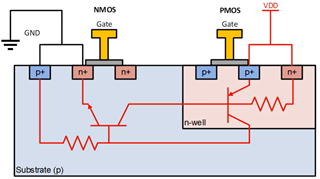
\includegraphics[width=0.7\textwidth]{chapter2/latchup.png}
    \caption{Example of a latch-up event. Reproduced from~\cite{TI_latchup}.}\label{fig:latchup}
\end{figure}

Fast-switching output stages are particularly susceptible because voltage overshoot, undershoot, capacitive coupling, or current injection from pad and \ac{ESD} structures can disturb the local substrate and well potentials \cite{baker,dally_poulton_1998}. Latch-up susceptibility is reduced by lowering the effective substrate and well resistances through closely spaced and sufficiently numerous well and substrate contacts. Guard rings are also commonly used to collect injected carriers before they can trigger the parasitic structure. A p$^+$ guard ring connected to $V_{SS}$ can be placed around NMOS devices, while an n$^+$ well guard ring connected to $V_{DD}$ can protect PMOS devices~\cite{layout_fundamentals,baker}.
        
\section{Chapter Summary}

This chapter presented the fundamental concepts required for the design and analysis of a high-speed serial-link \ac{TX}. The discussion began with the evolution from parallel to serial communication links and introduced the advantages of differential signaling for high-speed data transmission. \ac{NRZ} encoding was then examined in terms of its time- and frequency-domain characteristics, followed by an overview of the \ac{USB} standard and the relevant \ac{USB}~3.2 physical-layer requirements considered throughout this work.

The main \ac{SI} limitations associated with multi-gigabit communication were subsequently discussed. \ac{ISI} was related to the bandwidth-limited and frequency-dependent behavior of the transmission channel, while insertion loss, return loss, impedance discontinuities, jitter, and finite slew rate were introduced as important mechanisms that degrade the transmitted waveform. Transmission-line behavior and scattering parameters were presented as tools for characterizing the communication channel, and the eye diagram was introduced as a practical means of evaluating the resulting voltage and timing margins. Based on these limitations, \ac{TX} and \ac{RX} equalization techniques were discussed, with particular emphasis on \ac{TX}-side feed-forward equalization. The operation of a finite-impulse-response equalizer was described through delayed and weighted replicas of the transmitted data, including the use of pre-cursor, main-cursor, and post-cursor taps to compensate for channel-induced \ac{ISI}.

The chapter also introduced the output-driver architectures considered for high-speed \acsp{TX}. \ac{CML} and \ac{VMD} were described in terms of their operating principles, output termination, differential swing, and power consumption. Their main trade-offs were then compared, showing that \ac{CML} provides straightforward impedance control and implementation of multi-tap \ac{FFE} at the expense of continuous static current, whereas voltage-mode and \ac{SST} drivers can achieve improved power efficiency but require greater attention to output-impedance calibration and equalizer segmentation.

Finally, the discussion was extended from schematic-level design to physical implementation. The \ac{IC} design methodology and the influence of layout parasitics were introduced, followed by device-sizing and matching techniques intended to reduce systematic and random mismatch. Layout-dependent effects such as the \ac{WPE} and \ac{LOD} effect were considered, together with routing-related limitations including IR drop, parasitic capacitance, \ac{EM}, and latch-up. Particular attention was given to differential-routing symmetry, since unequal interconnect resistance and capacitance between complementary signal paths can introduce different RC time constants and consequently degrade the timing and waveform symmetry of high-speed differential signals.

These concepts establish the theoretical and physical-design basis for the \ac{TX} architecture and circuit implementation presented in the following chapters.